\documentclass[14pt,oneside,final]{extreport}
\usepackage[utf8]{inputenc} 
\usepackage[english,russian]{babel}

\setlength\parindent{1.25cm} % Красная строка 1.25 см
\linespread{1.3} 			 % Мехстрочный интервал 1.5

\usepackage{vmargin}
\setpapersize{A4} % Размер страницы A4
\setmarginsrb{30mm}{20mm}{10mm }{20mm  }{0pt       }{0mm    }{0pt       }{13mm    }
%            {left}{top }{right}{bottom}{headheight}{headsep}{footheight}{footskip}
\usepackage{indentfirst}
\usepackage{pscyr}			 % Нормальные шрифты
\usepackage[T2A]{fontenc}	 % Поддержка русских букв
\usepackage{url}
\usepackage{float}
\usepackage{tabularx}
\usepackage{amsmath}
\usepackage{pdfpages}
\usepackage{tikz}
\usepackage{enumitem}
\usepackage{textcomp}
\usepackage{listings}
\usepackage{array}
\usepackage{longtable}
\usepackage{verbatim}
\usepackage[percent]{overpic}
\usepackage{multirow}
\usepackage{pbox}
\usepackage{listings}
\usepackage{lstautogobble}
\usepackage{placeins}
\usepackage{selectp}
\usepackage[figure,table]{totalcount}
\usepackage{lastpage}
\usepackage{textpos}
\usepackage{tabu}
\usepackage{textcomp}
\usepackage{gensymb}
\usepackage[toc]{appendix}
\usepackage{wrapfig}
\usepackage{afterpage}
\usepackage{totcount}
 %\usepackage{titlesec}
\usepackage{titlesec}

%Установка листингов
\lstset{basicstyle=\ttfamily,
	mathescape=true,
	escapeinside=||,
	tabsize=4,
	numbers=left,
	frame=tb,
	autogobble}

% Листинг без нумерации
\lstdefinestyle{nonumbers}{numbers=none}

% Новые типы столбцов для таблиц
\newcolumntype{Z}{>{\centering\let\newline\\\arraybackslash\hspace{0pt}}X} 
\newcolumntype{M}{>{\raggedright\let\newline\\\arraybackslash\hspace{0pt}}X}
\newcolumntype{L}[1]{>{\raggedright\let\newline\\\arraybackslash\hspace{0pt}}m{#1}}
\newcolumntype{C}[1]{>{\centering\let\newline\\\arraybackslash\hspace{0pt}}m{#1}}

% Выравнивание названий таблиц и рисунков
\usepackage[nooneline]{caption}
\captionsetup[table]{justification=raggedleft} 
\captionsetup[figure]{justification=centering,labelsep=endash} 

% Формат заголовков
\usepackage{subcaption}
% 1го уровня
\titleformat{\chapter}[display]
{\normalfont\raggedright\bfseries}
{}
{0pt}
{\thechapter\enskip}
[]
% Не нумерованые секции 1го уровня
\titleformat{name=\chapter,numberless}[hang]
{\normalfont\centering\bfseries}
{}
{0em}
{
	\MakeUppercase 	
}

% 2го уровня     
\titleformat{\section}
{\normalsize\bfseries}
{\thesection}
{1em}{}
% 3го уровня     
\titleformat{\subsection}
{\normalsize}
{\thesubsection}
{1em}{}




   
% Настройка вертикальных и горизонтальных отступов для заголовков
\titlespacing*{\chapter}{0pt}{-9mm}{8pt} % -9 мм чтобы получить 20 мм от верхнего края стр
\titlespacing*{\section}{\parindent}{*4}{*4}
\titlespacing*{\subsection}{\parindent}{*2}{*2}
    
% сквозная нумерация
\usepackage{chngcntr}
\counterwithout{figure}{chapter}
% сквозная нумерация формул
\renewcommand{\theequation}{\thechapter.\arabic{equation}}

\renewcommand{\thefigure}{\arabic{figure}}
\usepackage[tableposition=top]{caption}
\usepackage{subcaption}
\DeclareCaptionLabelFormat{gostfigure}{Рисунок #2}
\DeclareCaptionLabelFormat{gosttable}{Таблица #2}
\DeclareCaptionLabelSeparator{gost}{~---~}
\captionsetup{labelsep=gost}
\captionsetup[figure]{labelformat=gostfigure}
\captionsetup[table]{labelformat=gosttable}
\captionsetup{figurewithin=none, tablewithin=none} %сквозная нумерация таблиц
\renewcommand{\thesubfigure}{\asbuk{subfigure}}

% Для приложений
\renewcommand{\appendixtocname}{Приложения}
\renewcommand{\appendixpagename}{Приложения}

\makeatletter
\g@addto@macro\appendices{\renewcommand{\thechapter}{\Asbuk{chapter}}}
\makeatother

\usepackage[toc]{appendix}
    \renewcommand\appendixname{Приложение}
    \makeatletter
    \def\redeflsection{\def\l@section{\@dottedtocline{1}{1.5em}{7.8em}}}
    \renewcommand\appendix{\par
    \setcounter{section}{0}%
    \setcounter{subsection}{0}%
    \def\@chapapp{\appendixname}%
     %\addtocontents{toc}{\protect\redeflsection}
    \def\thesection{\appendixname\hspace{0.2cm}\@arabic\c@section}}
    \makeatother
\sloppy

\usepackage[titles]{tocloft}
\renewcommand{\contentsname}{Содержание}
\renewcommand{\cfttoctitlefont}{\normalfont\bfseries\MakeUppercase}
\renewcommand\cftchapfont{\mdseries}
\renewcommand\cftchappagefont{\mdseries}
 %\setlength\textwidth{3in} % just for this example                                             % below code (e.g vertical space)


%\let\LaTeXStandardTableOfContents\tableofcontents
%\renewcommand{\tableofcontents}{%
%	\begingroup%
%	\renewcommand{\bfseries}{\relax}%
%	\LaTeXStandardTableOfContents%
%	\endgroup%
%}%

% Счетчик источников
\newtotcounter{citnum}
\def\oldbibitem{} \let\oldbibitem=\bibitem
\def\bibitem{\stepcounter{citnum}\oldbibitem}

\newcommand*\minus{\item[--]} % Символ минус для списков
\newcommand{\rom}[1]{\uppercase\expandafter{\romannumeral #1\relax}} % Команда \rom для римских цифр

% Чтоб t! работал как надо (рисунок вверху стр)
\makeatletter
\setlength{\@fptop}{0pt}
\makeatother

\DeclareRobustCommand{\gobblefour}[4]{}
\newcommand*{\SkipTocEntry}{\addtocontents{toc}{\gobblefour}}

%определенные страницы
%\outputonly{97-102}
%\usepackage{ltablex}

\begin{document}
	\setboolean{@twoside}{false}
	\includepdf[pages=-,offset=73 -75,pagecommand={
	\clearpage
	\thispagestyle{empty}
		\begin{tikzpicture}[remember picture, overlay]
			\node at (8.00-0.5, -3.5) {\noindent Робототехника и комплексная автоматизация};
			\node at (8.00-0.5, -4.5) {Компьютерные системы автоматизации производства};
			\node at (7.00-0.5, -10.3) {Интегрированная система поддержки принятия решения о выборе};
			\node at (7.00-0.5, -11.1) {режимов механической обработки тонкостенных деталей};
			\node at (13.5-0.5, -14.52) {П.А. Еремейкин};
			\node at (2.00-0.5, -14.5) {РК9-121};
			\node at (13.6-0.5, -15.8) {А.Д. Жаргалова};
			\node at (13.4-0.5, -21.30) {Л.А. Силаева};
			\node at (13.4-0.5, -22.7) {А.С. Козодаев};
		\end{tikzpicture}}]{titul.pdf}

	\setboolean{@twoside}{false}
	\includepdf[pages=-,offset=73 -75,pagecommand={
	\clearpage
	\thispagestyle{empty}
		\begin{tikzpicture}[remember picture, overlay]
			\node at (14.7-0.5, -3.67) {РК9};
			\node at (3.40-0.5, -8.3) {РК9-121};
			\node at (7.40-0.5, -9.3) {Еремейкин Петр Александрович};
			\node at (9.70-0.5, -10.75) {Интегрированная~~~система~~~поддержки~~~принятия};
			\node at (7.00-0.5, -11.45) {решения~~о~~выборе~~режимов~~механической~~обработки~~тонкостенных};
			\node at (-0.3-0.5, -12.15) {деталей};
			\node at (3.30-0.5, -18.45) {Техническое задание};
			\node at (3.05-0.5, -19.05) {1. Определить основания разработки};
			\node at (3.70-0.5, -19.6) {2. Сформулировать назначение разработки};
			\node at (7.38-0.5, -20.18) {3. Выявить требования к функциональным характеристикам и надежности};
			\node at (3.00-0.5, -20.72) {4. Установить условия эксплуатации};
			\node at (3.70-0.5, -21.27) {5. Определить стадии и этапы разработки};
			\node at (4.60-0.5, -21.82) {Концептуальное проектирование};
			\node at (7.20-0.5, -22.39) {1. Выбор методов создания интегрированной~~системы~поддержки~приня-};
			\node at (1.50-0.5, -22.94) {тия решений (ИСППР)};
			\node at (7.23-0.5, -23.49) {2. Выбор языка программирования, модульной платформы и системы мо- };
			\node at (0.30-0.5, -24.14) {делирования};
			\node at (2.45-0.5, -24.65) {3. Формулировка целей и задач};
		\end{tikzpicture}}]{task1.pdf}
	
	\setboolean{@twoside}{false}
	\includepdf[pages=-,offset=73 -75,pagecommand={
		\clearpage
		\thispagestyle{empty}
		\begin{tikzpicture}[remember picture, overlay]
%		\draw[very thin,color=gray] (-100,-100) grid (100,100);
		\node at (3.90-0.5, 0.11) {Эскизное проектирование};
		\node at (3.40-0.5, -0.47) {1. Разработать функциональную модель};
		\node at (7.40-0.5, -1.03) {2. Разработать структуру входных и выходных данных для анализа дефор-};
		\node at (-0.5-0.5, -1.58) {маций};
		\node at (7.40-0.5, -2.13) {3. Определить набор~~входных параметров для модуля калькулятора режи-};
		\node at (0.20-0.5, -2.74) {мов резания};
		\node at (3.70-0.5, -3.28) {Рабочее проектирование};
		\node at (5.87-0.5, -3.82) {1. Разработать информационную модель (диаграмму классов)};
		\node at (7.30-0.5, -4.37) {2. Реализовать~~модули~~в программном~~коде:~~а) калькулятор р.р. б) мо-};
		\node at (7.30-0.5, -4.92) {дуль~~CAE~~расчета в) модуль визуального отображения г) модуль вывода};
		\node at (3.90-0.5, -5.47) {результатов моделирования в .docx формате};
		\node at (7.20-0.5, -7.13) {Расчет затрат на создание интегрированной системы поддержки принятия};
		\node at (-0.3-0.5, -7.7) {решений};
		\node at (7.00-0.5, -11.35) {Провести~~анализ~~опасных~~и~~вредных~~факторов,~~воздействующих на};
		\node at (7.20-0.5, -11.95) {пользователя~~интегрированной~~системы~~поддержки~~принятия решения,};
		\node at (7.12-0.5, -12.52) {выполнить расчет заземления, выбрать рациональный способ утилизации};
		\node at (0.40-0.5, -13.1) {печатных плат};
		\node at (13.5-0.5, -23) {А.Д. Жаргалова};
		\node at (13.5-0.5, -24.15) {П.А. Еремейкин};
		\end{tikzpicture}}]{task2.pdf}

	\setboolean{@twoside}{false}
	\includepdf[pages=-,offset=73 -75,pagecommand={
		\clearpage
		\thispagestyle{empty}
		\begin{tikzpicture}[remember picture, overlay]
		\node at (7.20-0.5, -7.05) {Еремейкин Петр Александрович};
		\node at (2.80-0.5, -2.7) {РК};
		\node at (2.80-0.5, -3.44) {РК9};
		\node at (2.80-0.5, -4.24) {РК9-121};
		\node at (9.70-0.5, -7.95) {Интегрированная~~~система~~~поддержки~~~принятия};
		\node at (7.00-0.5, -8.65) {решения~~о~~выборе~~режимов~~механической~~обработки~~тонкостенных};
		\node at (-0.3-0.5, -9.35) {деталей};
		\end{tikzpicture}}]{plan.pdf}
 
%	\begin{titlepage}
%		\vspace*{-2cm}
%		\begin{center}
%			\textbf{РЕЦЕНЗИЯ\\}
%			\vspace{0.8cm} 
%			на дипломный проект студента группы РК 9-121 МГТУ им. Н. Э. Баумана \\
%			Еремейкина Петра Александровича \\
%			на тему \\
%			<<Интегрированная система поддержки принятия решения о выборе режимов механической обработки тонкостенных деталей>>
%		\end{center}
%		
%		Дипломный проект студента Еремейкина П. А. посвящён актуальной проблеме обработки тонкостенных деталей в условиях ограниченной номенклатуры применяемого оборудования. Рациональный выбор режимов резания с использованием разработанной интегрированной системы  позволит снизить затраты на обработку тонкостенных деталей в трехкулачковом патроне.
%		
%		В дипломном проекте убедительно раскрыты преимущества методики назначения ``мягких'' режимов резания перед традиционными способами обработки тонкостенных деталей. Система поддержки принятия решения спроектирована в соответствии с современными тенденциями разработки ПО и позволяет упростить задачу назначения рациональных режимов резания. 
%		
%		Отмечаю большой вклад дипломника в исследование проблемы, разработку методики, проектирование и реализацию программных модулей системы. 
%		
%		В качестве недостатка проекта можно отметить существенные упрощения, принятые при разработке пробной модели токарной обработки.
%		
%		
%		В целом проект выполнен в соответствии с требованиями к дипломным проектам и заслуживает оценки отлично, а студент Еремейкин Петр Александрович присвоения квалификации инженер.\\
%
%		
%		\begin{textblock}{13}(0,0.4)  	\noindent Рецензент \hfill А. А. Караулов\vspace{0.8cm}\\
%			\noindent	Должность и место работы \hfill <заполнить>\vspace{0.8cm}\\
%			\noindent	Подпись  А. А. Караулова заверяю. \hfill <заполнить> \\
%			\noindent	<заполнить> \hfill 
%		\end{textblock}
%		
%		\thispagestyle{empty}
%	\end{titlepage}


	\renewcommand*\contentsname{\hfill Содержание \hfill}
	\clearpage
	\setcounter{page}{2}
	\tableofcontents
	

	\chapter*{Аннотация}
	\addcontentsline{toc}{chapter}{\MakeUppercase{Аннотация}}
		
	Расчетно-пояснительная записка к дипломному проекту «Интегрированная система поддержки принятия решения о выборе режимов механической обработки тонкостенных деталей» содержит \pageref{LastPage} страниц машинописного текста, \totalfigures\ рисунков, \totaltables\ таблиц,  	\total{citnum}\ источников, 2 приложения.
		
	В расчетно-пояснительной записке описаны предпосылки создания системы, подробно рассмотрены этапы проектирования. Также уделено внимание техническим средствам разработки: системам управления базами данных, языкам программирования, программным платформам и библиотекам. Организационно-экономическая часть записки посвящена определению затрат на разработку интегрированной системы поддержки принятия решения. Кроме того, рассмотрены вопросы охраны труда пользователя системы: определены вредные и опасные факторы, способы снижения их воздействия, а также рассчитана  система защитного заземления. В экологической части расчетно-пояснительной записки описаны способы утилизации печатных плат.

	\newpage		
	
	\chapter*{Введение}
	\addcontentsline{toc}{chapter}{\MakeUppercase{Введение}}
	Эксплуатационные характеристики изделий машиностроения в большой мере зависят от качества изготовления деталей, составляющих изделие. Качество изготовления определяется степенью соответствия параметров готовой детали и параметров, достижение которых требуется документацией. В роли такого параметра может выступать точность изготовления геометрических размеров, определяемая допуском. 
	
	Погрешности различных видов препятствуют абсолютно точному воспроизведению заданных параметров. Например, на точность изготовления деталей влияют погрешности базирования, измерения, настройки инструмента и т.д. При обработке нежестких деталей на первый план выходят погрешности, связанные с деформацией самой детали.
	
	Рассмотрим пример обработки тонкостенной детали в трехкулачковом патроне токарного станка. Схема обработки изображена на рисунке~\ref{fig:scheme}. Цифровыми сносками обозначены: 1~-~кулачок патрона, 2~-~цилиндрическая заготовка, 3~-~токарный резец. До начала обработки деталь находится в недеформированном состоянии (рисунок~\ref{fig:scheme-a}). После закрепления детали силы, действующие со стороны кулачков, деформируют заготовку таким образом, что профиль заготовки отличается от идеально цилиндрического (рисунок~\ref{fig:scheme-b}). Дополнительно заготовка деформируется под действием силы резания, а также в связи с нагревом. В процессе резания инструмент неравномерно снимает припуск по окружности заготовки (рисунок~\ref{fig:scheme-c}). После окончания обработки и снятия усилий закрепления отклонение от круглости заготовки достигает величин, сравнимых с величиной допуска и в зависимости от конкретных условий может превышать его (рисунок~\ref{fig:scheme-d}).
	
	\begin{figure*}[t!]
	    \centering
	    \begin{subfigure}[t]{0.5\textwidth}
	        \centering
        	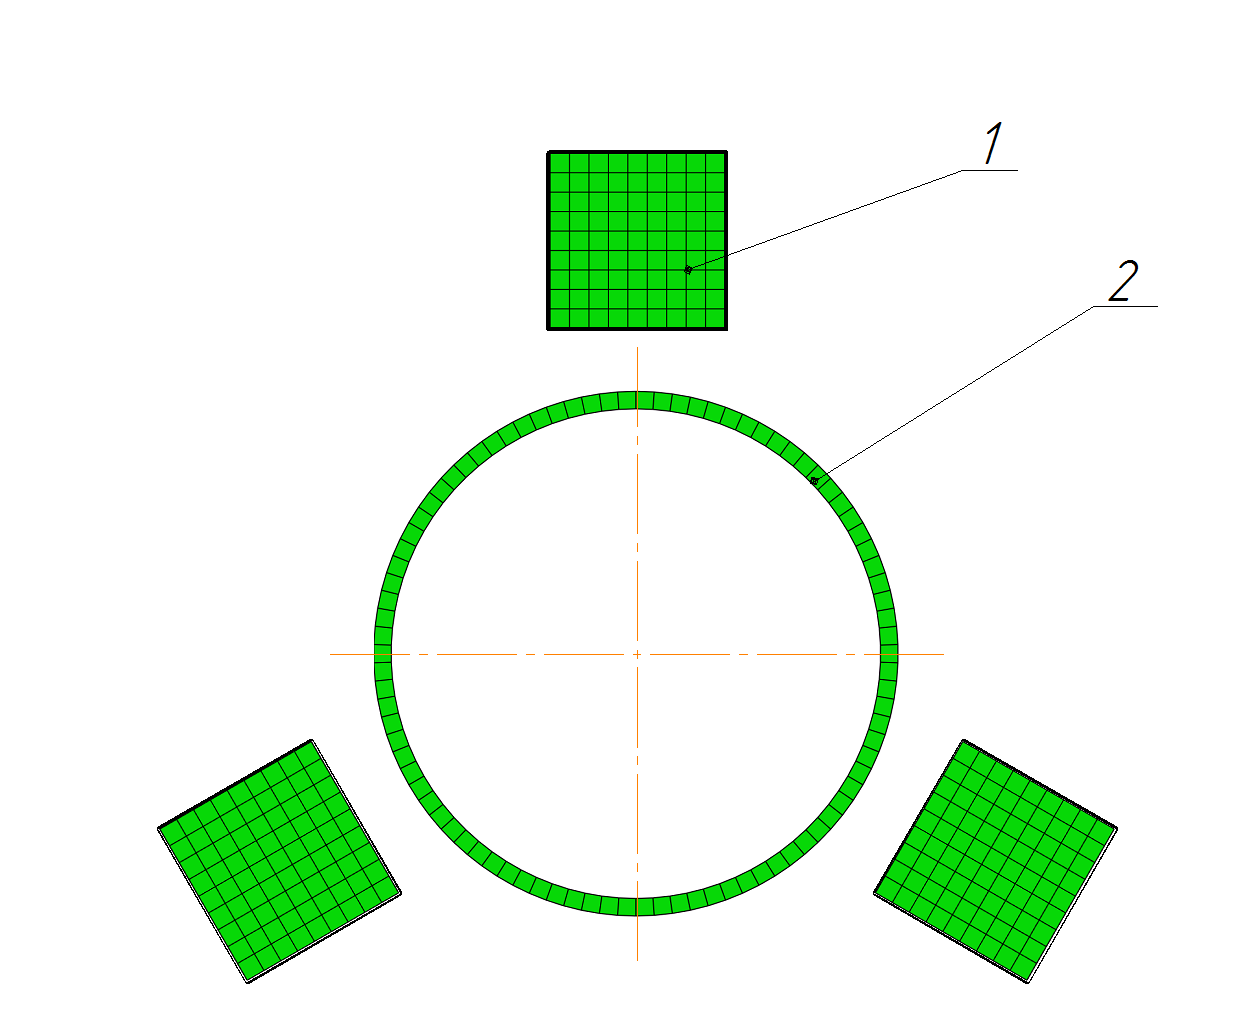
\includegraphics[scale=0.25]{img/scheme-a}
	        \caption{До закрепления}
	        \label{fig:scheme-a}
	    \end{subfigure}%
	    ~ 
	    \begin{subfigure}[t]{0.5\textwidth}
	        \centering
        	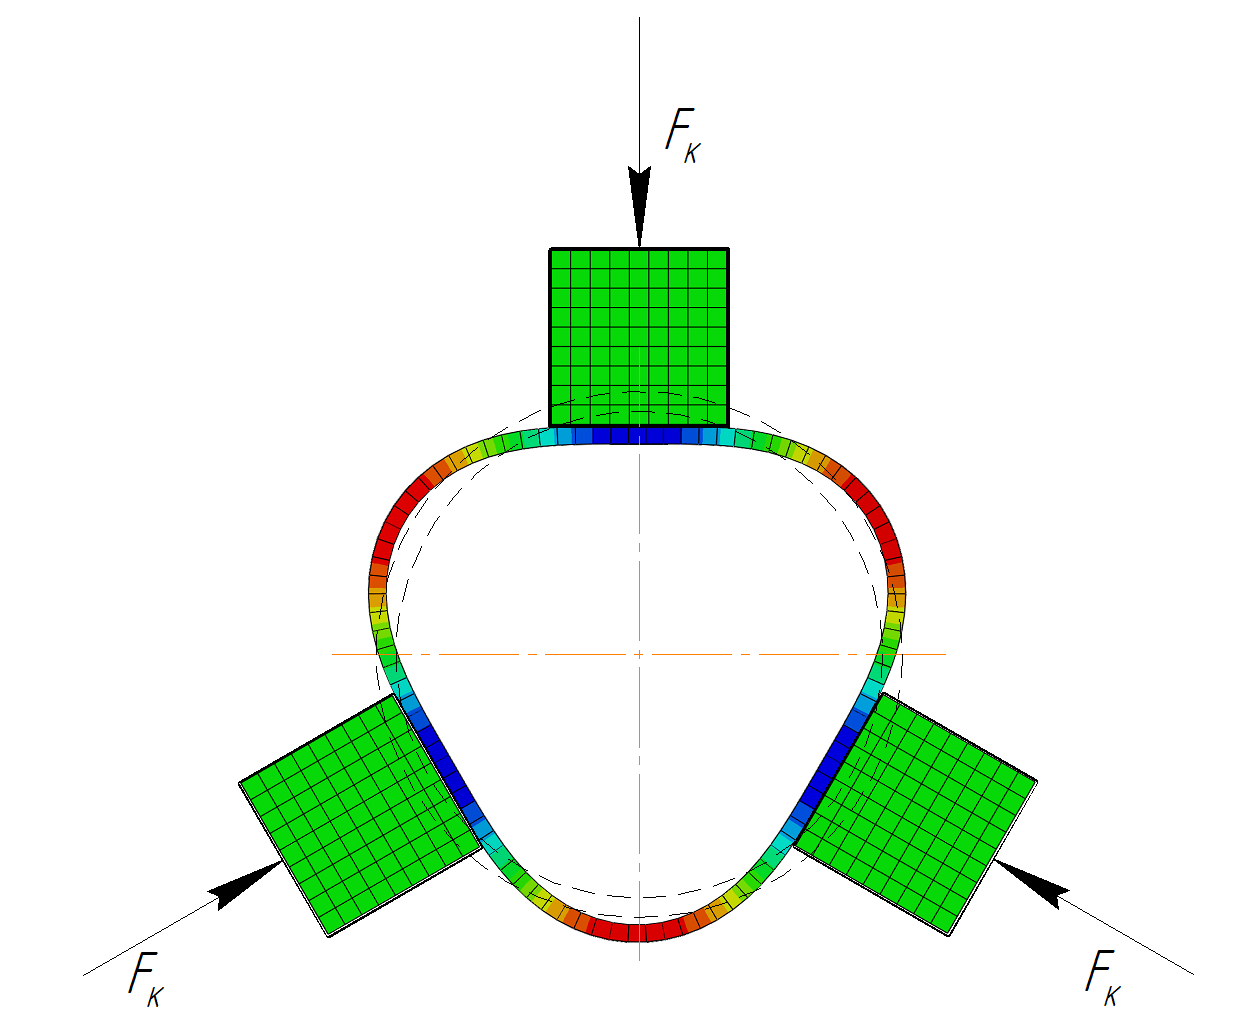
\includegraphics[scale=0.25]{img/scheme-b}
        	\caption{Закрепленная заготовка} \label{fig:scheme-b}
	    \end{subfigure}
	    
 	    \begin{subfigure}[t]{0.5\textwidth}
   	        \centering
           	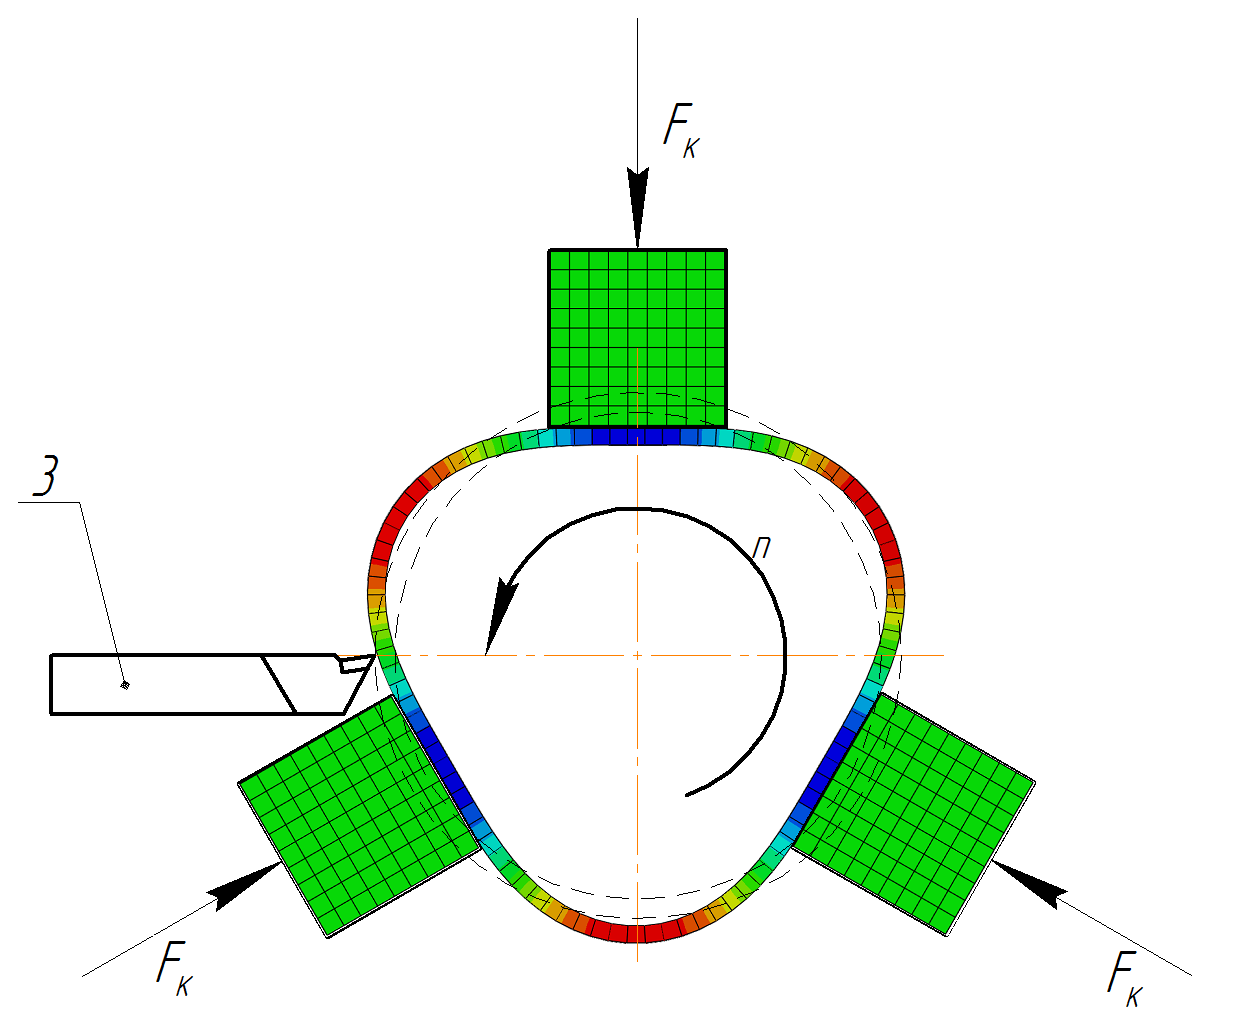
\includegraphics[scale=0.25]{img/scheme-c}
           	\caption{Обработка} \label{fig:scheme-c}
   	    \end{subfigure}%
   	    ~
   	    \begin{subfigure}[t]{0.5\textwidth}
   	       	\centering
   	        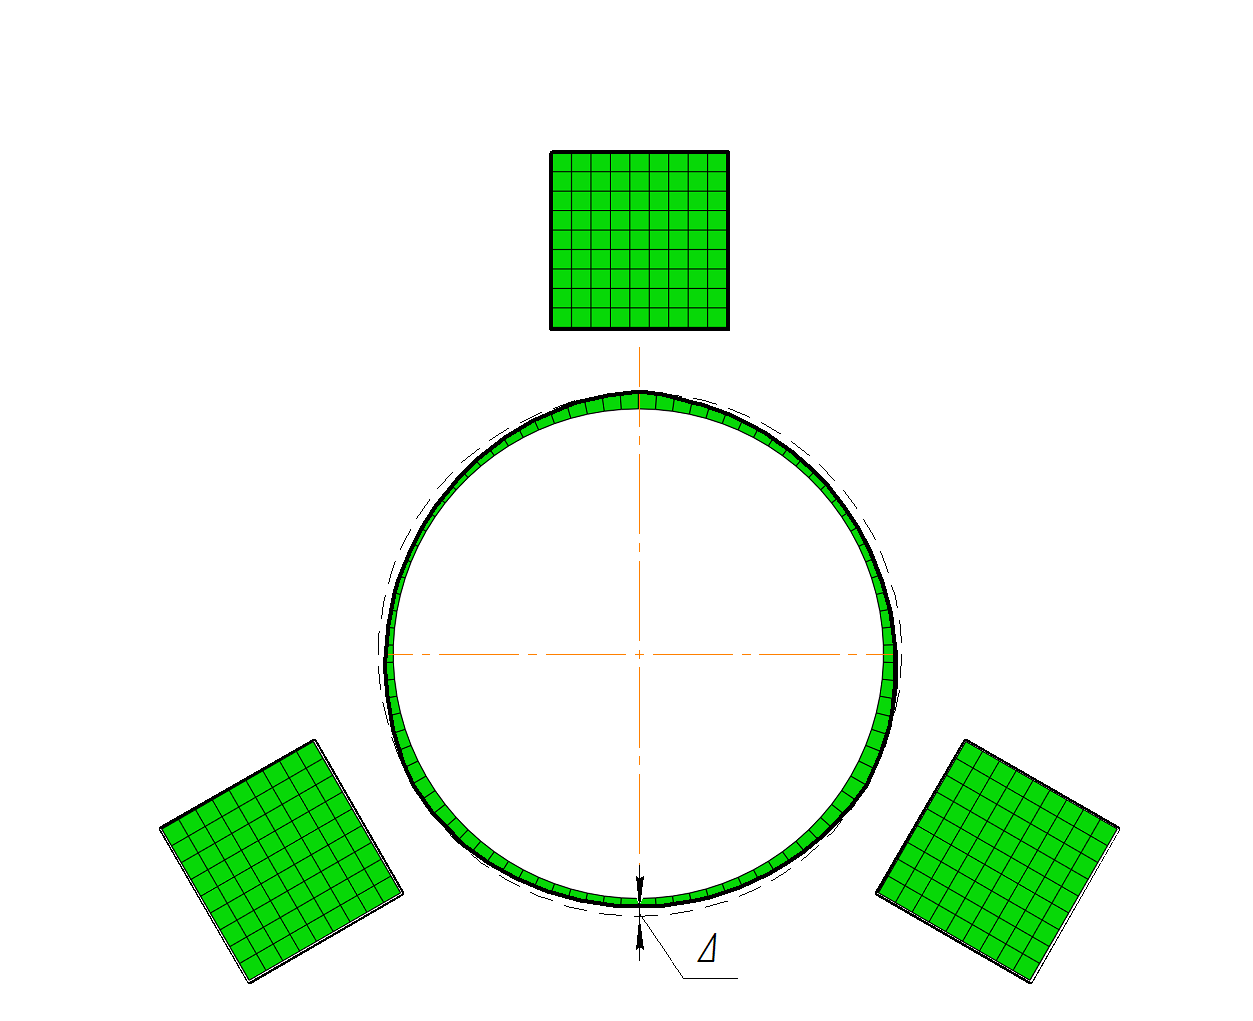
\includegraphics[scale=0.25]{img/scheme-d}
   	    	\caption{Результат} \label{fig:scheme-d}
	   	\end{subfigure}
	    \caption{Обработка тонкостенной заготовки} \label{fig:scheme}
	\end{figure*}


	На практике в случае обработки нежестких деталей применяется специальное технологическое оборудование, позволяющее уменьшить возникающие деформации. Использование сырых кулачков, растрачиваемых под диаметр заготовки - один из способов уменьшения деформаций закрепления. После растачивания кулачок охватывает деталь по большей площади. Также используется обработка с технологическим заполнителем (например, легкоплавким материалом), который увеличивает жесткость детали на время обработки и выплавляется после окончания обработки. Вариант обработки на нормативных режимах резания в специальных приспособлениях привлекателен тем, что он позволяет применять апробированные технологические процессы. Однако, необходимость создания при этом специальных приспособлений требует значительных материальных, производственных и временных затрат. Это удорожает технологическую подготовку производства и увеличивает её сроки. Подробный обзор существующих методов приведен в таблице \ref{tab:review}.

	\afterpage{%		
	% настройки для framebox
	\setlength{\fboxsep}{2pt}
	\setlength{\fboxrule}{0pt}
	\begin{small}
		\begin{longtabu} to \textwidth {|p{8cm}|p{8cm}|}
			\caption{Обзор методов обработки}
			\label{tab:review}\\
			\hline
			\qquad \qquad \quad Разжимная оправка & \qquad \qquad \qquad Сырые кулачки\\
			\hline
			\vspace{-3cm}\framebox{\qquad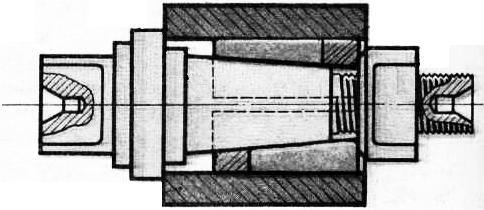
\includegraphics[scale=0.35]{img/opravka}} & \framebox{\qquad\qquad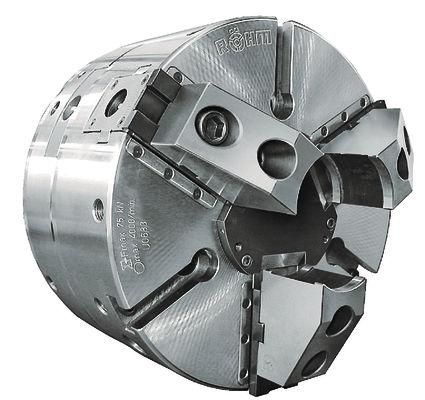
\includegraphics[scale=0.25]{img/raw-jaw}} \\
			%\hline 
			\qquad Разжимная оправка позволяет закрепить заготовку без существенных деформаций. Для этого используется цанга с продольными прорезями, которая разжи- мается конической поверхностью.
			Недостатки метода: ограниченная область применения; дополнительные затраты на покупку оправок под разные диаметры; дополнительные затраты на хранение оправок; временные затраты при смене оснастки \vspace{3mm} & \qquad Сырые кулачки могут быть использованы с трехкулачковым патроном для увеличения площади охвата заготовки. Сырые кулачки растачиваются под определенный диаметр. Недостатки метода:
			дополнительные затраты на растачивание кулачков; дополнительные затраты на закупку и хранение кулачков под различные диаметры; затраты на смену кулачков. \\ \hline
			\qquad Технологический заполнитель & \qquad ``Мягкие'' режимы резания\\
			\hline
			\vspace{-4cm}\framebox{\qquad\qquad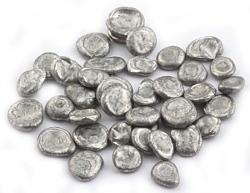
\includegraphics[scale=0.35]{img/wood-alloy}} & \framebox{\qquad\qquad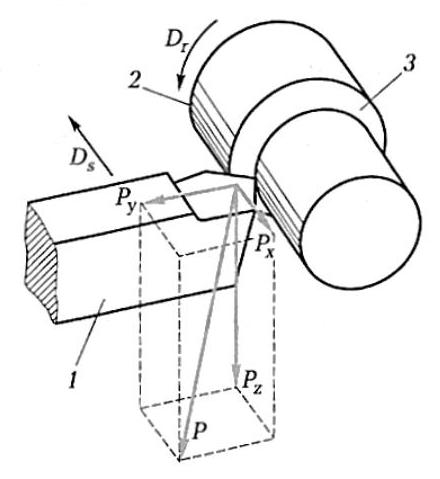
\includegraphics[scale=0.25]{img/cutting}} \\
			Технологический заполнитель используется для временного повышения жесткости заготовки. Например, в качестве заполнителя может быть использован легкоплавкий сплав Вуда ($ T_\textup{пл}=68,5 \degree C $). Недостатки метода: большинство технологи- ческих заполнителей токсичны (содержат кадмий); требуются специальные меры хранения; увеличение время подготовки к обработке & Разрабатываемый подход основан на назначении таких режимов резания, чтобы минимизировать деформаци деформации при обработке. При этом используется широко распростроненный трехкулачковый патрон, дополнительная оснастка не требуется. Недостатки метода: необходимость создания  специального ПО.
			\\
			\hline 
		\end{longtabu}
	\end{small}
	\clearpage
	}
	Ввиду указанных ограничений на существующие способы обработки, предлагается рассмотреть еще один метод - подбор режимов обработки и условий закрепления таким образом, чтобы обеспечить изготовление размеров в рамках допуска. Предполагается, что такой метод может найти применение прежде всего в единичном и мелкосерийном производстве, располагающим, как правило, только универсальным оборудованием. Суть подхода заключается в том, чтобы заранее, на этапе разработки технологической документации, определить режимы резания, менее эффективные с точки зрения производительности, но оптимальные с точки зрения точности изготовления. С уменьшением сил резания уменьшаются и деформации заготовки, а также требуемые усилия закрепления, но с другой стороны, увеличивается время обработки.  Подобрав баланс между скоростью и точностью обработки, технолог имеет возможность назначить режимы резания, приемлемые для изготовления заданной детали без привлечения дополнительной технологической оснастки.  Достоинством такого подхода является меньшая ресурсоёмкость и продолжительность технологической подготовки производства. Однако, данный подход в настоящее время ещё не получил достаточного научного обоснования и, как следствие, не поддержан методическими рекомендациями, необходимыми для его применения в промышленных масштабах \cite{article:zhargalova}.
	
	Для поддержки решения о назначении режимов резания предлагается разработать информационную систему, позволяющую анализировать деформации заготовки при заданных геометрических параметрах и режимах резания. Такой инструмент можно использовать для последовательной проверки ряда значений параметров процесса и выбора наиболее рациональных. 
	
	Система, спроектированная в соответствии с современными тенденциями в разработке ПО станет эффективным инструментом для назначения режимов обработки. Объектно-ориентированная модульная архитектура такой системы позволит расширять её функционал в случае возникновения новых требований к применению программы, а независимость от конкретной операционной системы позволит легко внедрить такие системы в процесс разработки технологической документации на предприятиях безотносительно конкретной существующей информационной среды.
	
	
	\chapter{Техническое задание}	
	
	\section{Основания для разработки}
	Основанием для разработки системы являются документы:
	\begin{enumerate}
	\item Задание на выполнение дипломного проекта
	\item Календарный план на выполнение дипломного проекта
	\end{enumerate}
	
	\section{Назначение разработки}
	Функциональным назначением разработки является обеспечение интегрированной рабочей среды для гибкого моделирования процессов деформирования тонкостенных заготовок в процессе их токарной обработки. Под гибкостью понимается возможность изменения параметров процесса в зависимости от расчетного случая и конфигурации заготовки. Эксплуатационным назначением является обеспечение инструментального средства для последовательного определения рациональных режимов резания тонкостенных заготовок и автоматизация сопутствующих расчетов.
	
	\section{Требования к функциональным характеристикам}
	    Система информационной поддержки должна обеспечивать выполнение следующих функций:
	\begin{enumerate}
	\item Расчет деформаций тонкостенной заготовки при токарной обработке с закреплением в кулачковом патроне.
	\item 	Автоматизация необходимых сопутствующих расчетов (режимов резания)
	\item 	Изменение параметров рассматриваемого процесса: геометрии заготовки  и оснастки и значений силовых факторов (силы резания и закрепления)
	\item 	Представление результатов расчета в виде графиков или таблиц деформаций
	\item 	Генерация отчета по результатам расчета
	\item 	Вывод дополнительных информационных отладочных сообщений 
	\end{enumerate}

	\section{Требования к надежности}
	Разрабатываемая система должна обеспечивать надежную работу в условиях ошибочного пользовательского ввода. При возникновении системных исключительных ситуаций необходимо обеспечить их обработку чтобы не допустить аварийного завершения программы.

	\section{Условия эксплуатации}
	Аппаратные   средства   должны   эксплуатироваться   в помещениях с выделенной розеточной электросетью 220В \(\pm\) 10\%, 50 Гц  с  защитным  заземлением  при  следующих  климатических условиях:
	\begin{itemize}
	\minus температура окружающей среды – от 15 до 30 градусов С;
	\minus относительная влажность воздуха -- от 30\% до 80\%;
	\minus атмосферное давление -- от 630 мм. р.с. до 800 мм. р.с.
	\end{itemize}

	\section{Требования к составу и параметрам технических средств}
	Программный продукт должен работать на компьютерах со следующими характеристиками:
	\begin{itemize}
		\minus объем ОЗУ не менее 2 Гб;
		\minus объем жёсткого диска не менее 40 Гб;
		\minus микропроцессор с тактовой частотой не менее 1.5 ГГц;
		\minus монитор с разрешением от 1024*768 и выше.
	\end{itemize}

	\section[Требования к информационной и программной совместимости]{Требования к информационной и программной \\совместимости}
	Разрабатываемая система должна работать на ПЭВМ под управлением Microsoft Windows 7. Требуется обеспечить работоспособность системы на платформе Java SE версии 8 Update 71 или новее. Минимальная версия Abaqus FEA 6.14-1.
	
	\section{Стадии и этапы разработки}
	Стадии разработки интегрированной системы поддержки принятия решения определяются ГОСТ 19.102-77 за исключением стадии ``Внедрение'', выполнение которой выходит за рамки дипломного проекта. Таким образом, разработка  состоит из 4 стадий:
	\begin{enumerate}
		\item Техническое задание
		\item Эскизный проект
		\item Технический проект
		\item Рабочий проект
	\end{enumerate}
	
	\section{Порядок контроля и приемки}
	Работоспособность системы проверяется через пользовательский интерфейс вручную.	При проведении контроля требуется проверка работоспособности четырех основных компонента системы: 
	\begin{itemize}
		\item Калькулятор режимов резания 
		\item Загрузчик моделей 
		\item Подсистема параметризации
		\item Подсистема моделирования
	\end{itemize}
	Для каждого компонента производятся испытания по характерным входным данным. 


	\chapter{Разработка концепции автоматизированной системы}
	\section{Принцип моделирования}
	Согласно техническому заданию система должна обеспечить расчет деформаций тонкостенной заготовки в процессе токарной обработки. Токарная обработка характеризуется большим разнообразием возможных вариантов осуществления в зависимости от обрабатываемой поверхности и способа закрепления. Разработать и запрограммировать адекватную модель, основанную исключительно на математическом представлении известных теоретических закономерностях сопротивления материалов для каждого из возможных вариантов - чрезвычайно сложная задача с технической точки зрения. 
	
	Известно, что современные CAE системы позволяют успешно решать задачи определения деформаций и напряжений для объектов практически неограниченной сложности благодаря использованию метода конечных элементов (МКЭ). После разбиения рассматриваемых объектов на конечные элементы определенного типа и наложении ограничений на эти элементы согласно закономерностям предметной области задача сводится к решению системы из большого количества уравнений. Успех решения полученной системы уравнений как правило определяется только отведенным на решение временем работы ЭВМ. 
	
	Тем не менее, сама по себе реализация метода конечных элементов в разрабатываемом продукте не возможна из-за большой трудоемкости и требует огромной исследовательской и проектной работы целого коллектива профессионалов. Таким образом, наилучшим выходом из сложившейся ситуации представляется использование готовой CAE системы. Применение системы МКЭ расчета возможно, если она отвечает следующим трем основным требованиям:
	\begin{enumerate}
	\item Предоставляет возможность расчета заранее составленной модели под управлением внешнего процесса операционной системы (в роли которого будет выступать разрабатываемая система анализа деформаций)
	\item Имеет механизмы параметризации модели. В наилучшем случае параметризация должна достигаться благодаря выполнению пользовательских сценариев.
	\item Позволяет получить результат расчета в виде графиков, диаграмм напряжений и деформаций, а также в числовом виде для каждого элемента модели.
	\end{enumerate}
		
	В рамках перечисленных соображений можно сформулировать концепцию системы следующим образом. На первом этапе система собирает информацию о значениях параметров модели через графический пользовательский интерфейс. По завершению ввода функция системы состоит в формировании задания для используемой готовой CAE системы. На этапе подготовки задания производится дополнительный расчет необходимых величин, если они не были непосредственно указаны на первом этапе и могут быть получены расчетным путем. Третий этап состоит в вызове расчетного ядра CAE системы по сформированному заданию. По завершению обработки модели разрабатываемая система агрегирует результаты и отображает их пользователю, при необходимости генерируя отчет.

	Таким образом, основная идея состоит в расчете модели обработки с использованием сторонней CAE системы. Предполагается, что роль разработчика моделей будет выполнять эксперт, как правило не являющийся пользователем системы. В задачи эксперта входит описание нового расчетного случая при помощи инструментов, предоставляемых конкретной выбранной системой МКЭ расчета и другие необходимые работы по подготовке системы. Готовая модель предоставляется в распоряжению пользователю, в задачи которого входит выбор наиболее подходящей модели из множества имеющихся и её загрузка в разрабатываемую систему поддержки.

	\section{Принцип модульности}
	Уже на этапе формулирования концепции системы становиться видна её большая сложность. Для того чтобы сохранить контроль над расширяющейся по мере разработке системы и не допустить её деградации следует определиться с принимаемыми для этого мерами и также включить их в концепцию системы, так как принимаемые меры коренным образом повлияют на процесс проектирования. 
	
	В соответствии с накопленным мировым опытом в разработке программного обеспечения одним из наиболее жизнеспособных способов контроля сложности является разработка приложения согласно принципам  объектно-ориентированного программирования. Во-первых,  ООП методология позволяет добиться большого процента повторного использования кода благодаря принципам наследования и полиморфизма \cite{Shildt}. Во-вторых, принципы абстракции и инкапсуляции облегчают задачу программиста так как они существенно ограничивают область кода, который влияет на рассматриваемый участок программы и позволяют формулировать мысли в терминах предметной области. 
	
	Разрабатываемая система сложна не только по причине большой трудоемкости процесса разработки, но также и процесса поддержки готовой системы. В случае возникновения новых функциональных требований, не покрытых техническим заданием на первом этапе, потребуется совершить большой объем работ, если заранее не предусмотреть модульность системы. Модульность системы позволит “присоединить” к готовой системе недостающие функциональные элементы - модули, без переработки какой-либо существенной части самого приложения. 
	
	Как показано выше, сам по себе переход от структурного программирования к объектно-ориентированному - большой шаг вперед. Однако, такой шаг ещё не гарантирует структурированной модульной архитектуры приложения. Отдельный класс хоть и инкапсулирует некоторые данные, тем не менее не является модулем в смысле всего приложения. Для достижения этой цели потребуется применение специальных мер, зависящих от выбранного языка программирования. Такие меры могут представлять, например, использование определенного набора шаблонов проектирования, в случае реализации модульности системы своими силами, или использования одного из многочисленных фреймворков в другом случае.  

	
	
	\section{Принцип комплексности}
	Принцип модульности оставляет широкие возможности для расширения функционала системы даже после выпуска готовой системы. Однако такой возможностью следует пользоваться в пределах разумного. Не следует исходить из этой концепции для оправдания отсутствия каких-либо востребованных функций. В контексте текущего проекта должен быть разработан исходный набор модулей, обеспечивающий выполнение большинства функций, которые могут понадобиться пользователю при работе в рамках рассматриваемой предметной области. Это означает что следует комплексно подойти к решению проблемы. 
	    
	В рамках базового набора модулей согласно техническому заданию должны обязательно присутствовать модуль для расчета режимов резания, модуль графического отображения результатов и модуль генерации отчетов. Также следует включить в основной состав модули просмотра трехмерного изображения рассчитываемой модели и вывода текстовой информации, формируемой CAE системой. 
	    
	Кроме самого факта наличия модулей в системе необходимо обеспечить взаимный обмен информацией между ними. Например, передачу значений, полученных в модуле расчета режимов резания в модуль параметризации модели. Этот прием позволит избавить пользователя от случайных ошибок при копировании и сделает работу с системой более удобной. Согласно идее комплексности, полезной особенностью может стать предоставление справочных данных для выбора в качестве значений вводимых параметров. 
	    
	Таким образом, разрабатываемая система должна стать результатом многосторонней проработки проблемы. 
	    

	\section{Принцип независимости}
	При разработке системы уже на самых ранних стадиях необходимо ориентироваться на возможное многообразие используемых на  предприятиях программных и аппаратных средств. Известно, что для  современного рынка информационных технологий характерна большая вариативность используемого программного обеспечения. В рамках проекта интерес представляют операционные системы и системы инженерных расчетов (CAE). Для разных предприятий сочетания конкретных решений в этих областях могут быть различными, например, роль операционной системы может выполнять какая либо версия Microsoft Windows или  Linux. В роли CAE системы может использоваться Ansys, Abaqus, в некоторых  случаях Siemens NX или SolidWorks. 
	
	В идеальном случае следует ориентироваться на независимость проектируемого приложения от индивидуальных особенностей какой-либо внешней системы. Это позволит расширить границы применения программы и облегчить задачу её освоения в рамках существующей информационной среды. Удовлетворить условиям концепции независимости поможет правильный выбор средств разработки, а также определенные проектные меры, например, разработка межсистемного взаимодействия на основе соглашений (интерфейсов). 
	
	\chapter{Предпроектное исследование}
	\section{Формулировка целей}
	Основной целью разработки является снижение трудоемкости назначения рациональных режимов резания. Эта цель может быть представлена в виде трех подцелей более низкого уровня: 
	\begin{enumerate}
	\item Снижение трудоемкости предварительных расчетов
	\item Снижение трудоемкости основных расчетов
	\item Снижение трудоемкости анализа результатов 
	\end{enumerate}
	\begin{figure}[!h]
	\begin{center}
	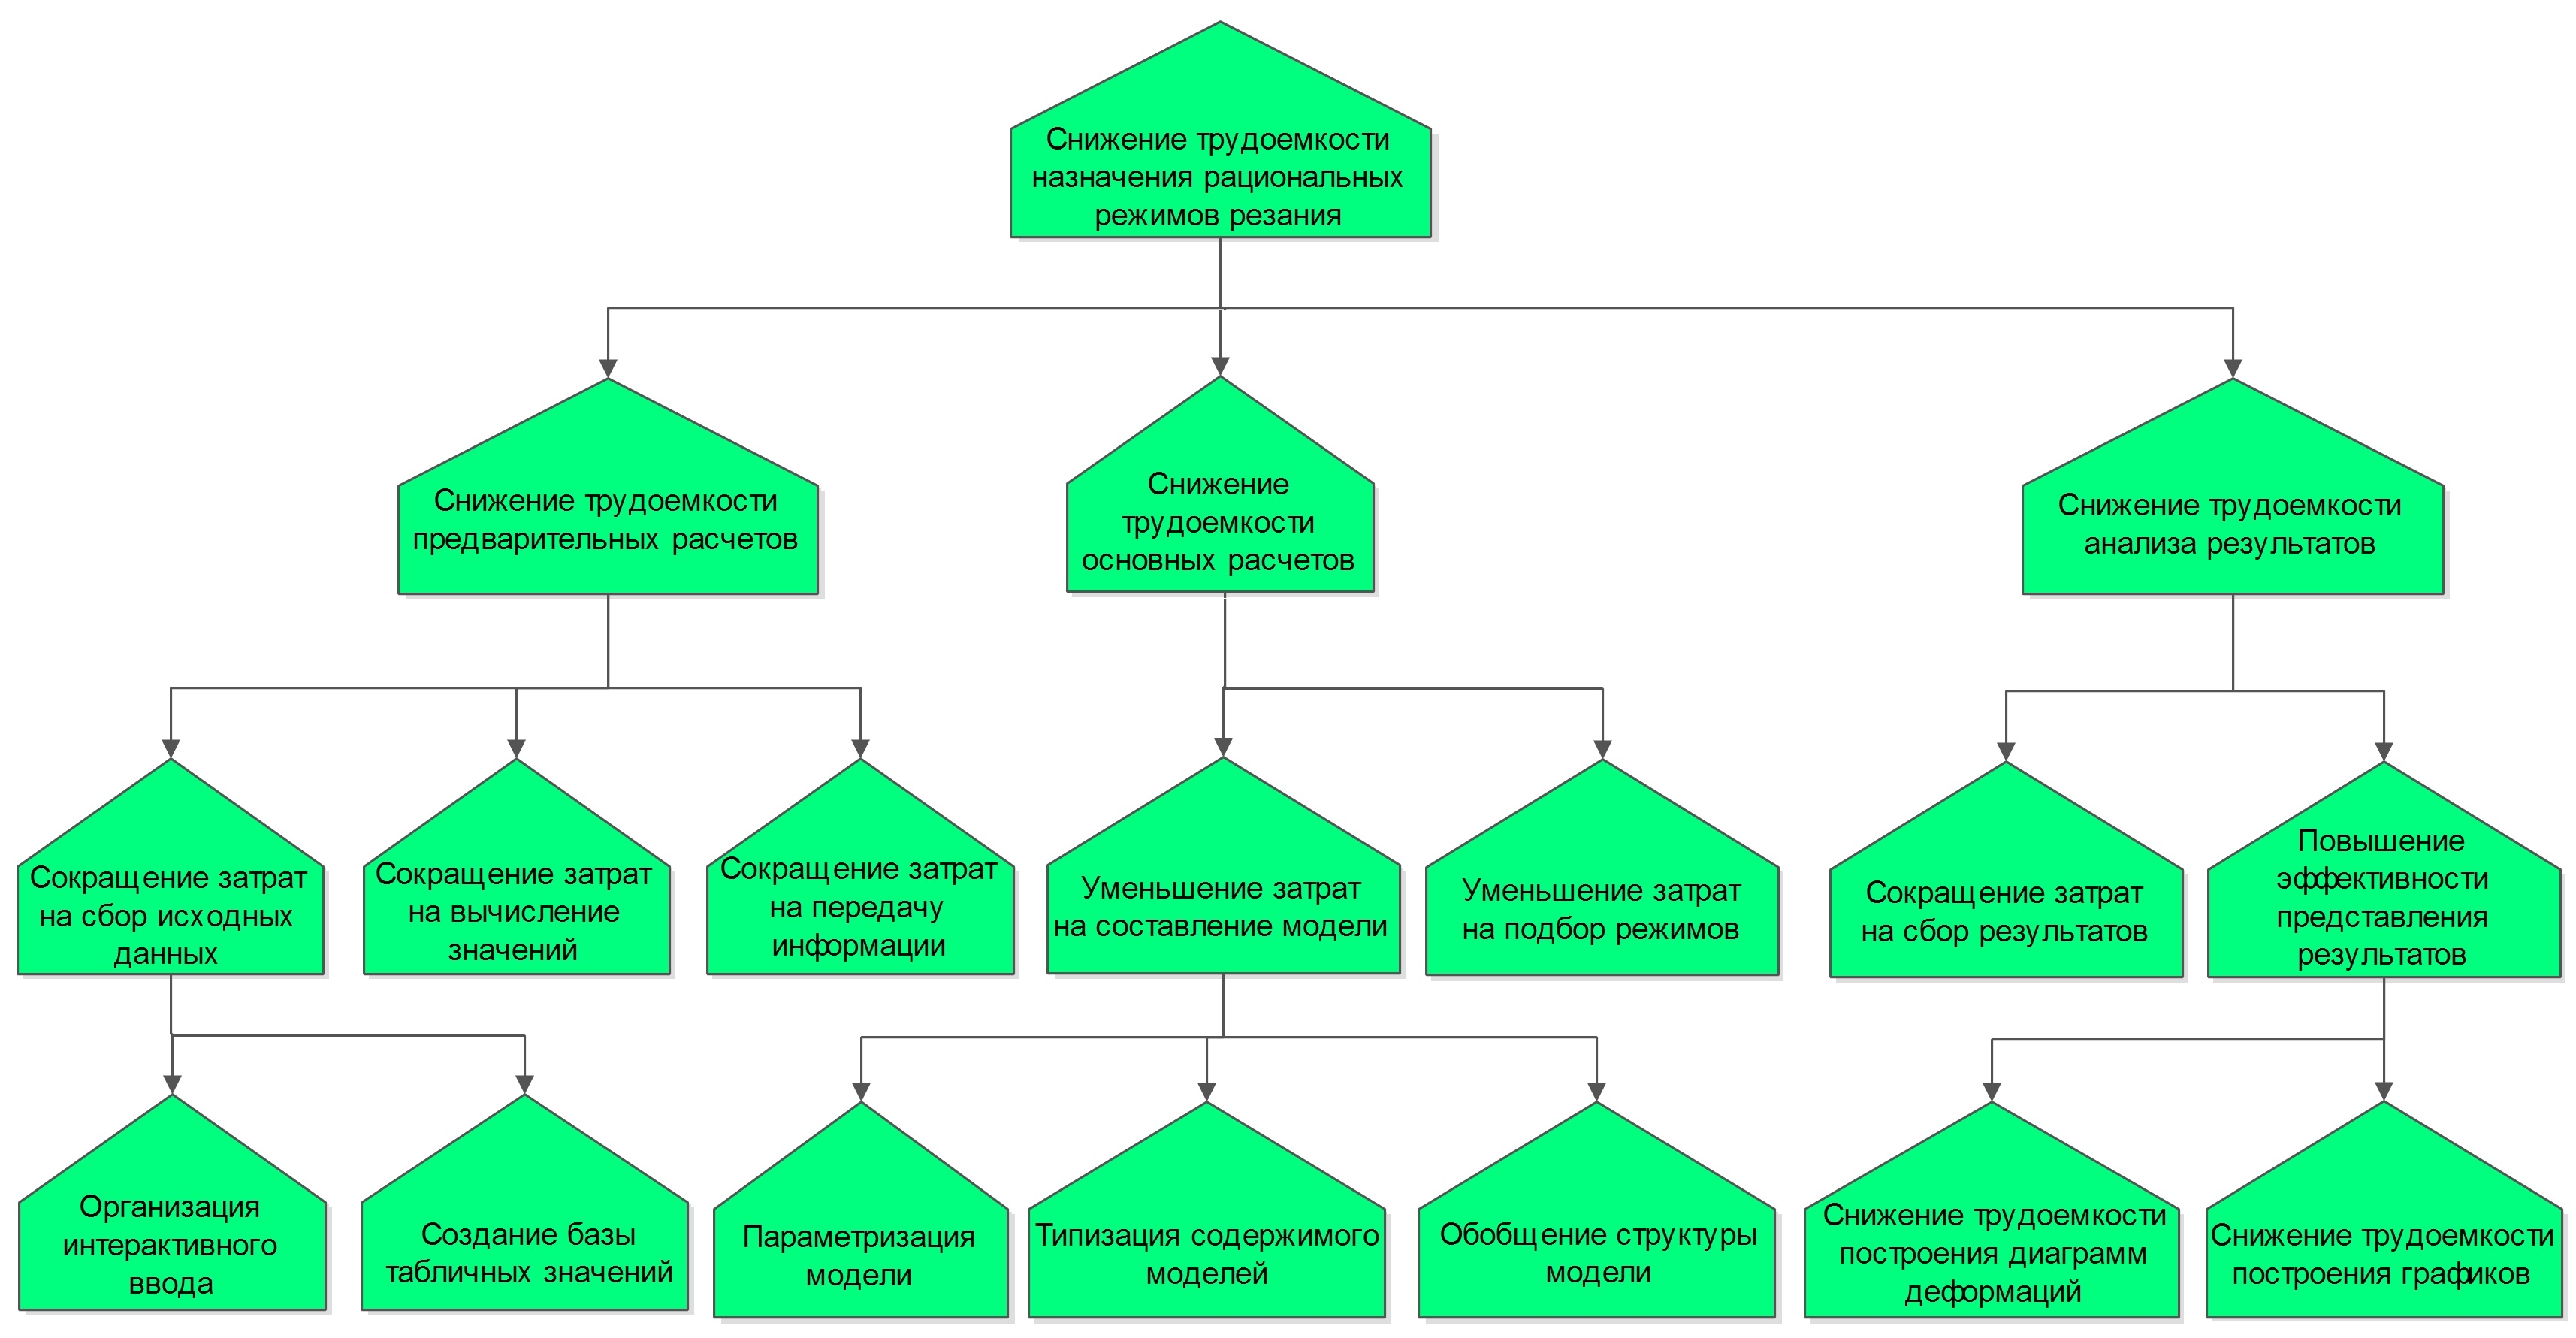
\includegraphics[scale=0.55]{img/at} 
	\end{center}
	\caption{Дерево целей}
	\label{fig:aim-tree}
	\end{figure}
	
	Снижение трудоемкости предварительных расчетов сводится к автоматизации вычисления режимов резания по традиционным методикам. Эта цель может быть достигнута при сокращении затрат на сбор исходных данных, вычисление значений и передачу информации. Под традиционными методиками понимается прежде всего таблично-аналитический подход, описанный в \cite{book:Kosilova}. Согласно указанной литературе, для вычисления параметров режима резания необходимо выбрать исходные данные из таблиц эмпирических коэффициентов и подставить их в приведенные в справочнике формулы. Снижение трудоемкости этих действий и образует первую подцель.
	
	Вторая задача состоит в том, чтобы разработать общую структуру модели, а также типизировать её содержимое. Путем параметризации может быть достигнуто эффективное повторное применение одной модели в рамках разработки различных технологических процессов. Используя внутренний расчетный механизм системы планируется обеспечить уменьшение затрат на подбор рациональных режимов резания. 
	
	После проведения расчетов требуется сделать вывод о допустимости принятых параметров обработки. Автоматизация построения диаграмм и графиков деформаций позволит повысить эффективность анализа результатов. 
	
	Дерево целей изображено на рисунке \ref{fig:aim-tree}. Оно систематизирует вышесказанное в виде иерархической структуры. 
		
	
				
	\section{Выбор языка программирования}
	Выбору языка программирования следует уделить особое внимание. От правильного решения существенно зависит насколько трудоемким будет процесс написания программы. Существующие языки программирования сильно различаются по возможностям, гибкости и области применения. На данном этапе необходимо рассмотреть основные варианты и выявить наилучший. 
	
	На стадии разработки концепции было выявлено, что следует опираться на подходы объектно-ориентированного программирования. Этот вывод соответствующим образом сужает область рассматриваемых решений. Для повышения пригодности продукта к обслуживанию также ограничимся общеизвестными и широко распространенными языками. Дополнительная выгода от использования таких языков состоит в возможности применения готовых компонентов и библиотек. 
	
	Под указанные ограничения подходят такие языки как С++, С\#, Java, Python. Сравним эти языки по существенным факторам методом непосредственной оценки. Для оценки будут приняты во внимание следующие характеристики: распространенность, скорость разработки, гибкость, безопасность. В рамках проекта производительность не рассматривается так как она не является ограничивающим фактором. По каждому критерию языку будет присвоен балл от 1 до 10. Наиболее предпочтительным будет признан язык с наибольшим суммарным баллом. 
	
	Распространенность может быть определена по числу проектов на информационном ресурсе github.com и числу заданных вопросов на stackoverflow.com. Эти ресурсы выбраны в качестве референтных из-за большой популярности в IT сообществе. Аналитическая фирма RedMonk опубликовала объективный рейтинг языков программирования в соответствии с указанными критериями \cite{web:RedMonk}. Этот отчет использован в качестве основания для присвоения баллов, поэтому Java получает максимальный балл, а остальные языки оценены меньшим числом. 
	
	Скорость разработки в большей мере субъективный параметр, так как он зависит не только от конструкций языка, но и от умений и опыта конкретного программиста, хотя можно выявить и общие тенденции. Скорость разработки рассматривается с учетом замечаний, изложенных в \cite{web:DZone}. Известно, что разработка на С++ требует больших временных затрат ввиду сложности конструкций и большого количества деталей, которые должны быть учтены программистом. По этому критерию предпочтение отдано Python, который относят к языкам сценариев. C\# и Java в плане скорости разработки не выделяются и получили средний балл.
	
	Гибкость также не поддается количественному определению, однако она зависит только от самого языка. Динамическая типизация позволила Python набрать максимальный балл. Также высоко оценены возможности ручного управления памятью в С++.
   
	\begin{table}[htb]
	\centering
	\caption{Оценка языков программирования}\label{tab:lang-rank} 
	\begin{tabularx}{\textwidth}{|l|Z|Z|Z|Z|}

		\hline Фактор & C++ & С\# & Java & Python \\ 
		\hline Распространенность & 9 & 9 & 10 & 9 \\ 
		\hline Скорость разработки & 8 & 9 & 9 & 10 \\ 
		\hline Гибкость & 10 & 9 & 9 & 10 \\ 
		\hline Безопасность & 8 & 10 & 10 & 8 \\ 
		\hline Итого & 36 & 37 & 38 & 37 \\ 
		\hline 
	\end{tabularx}
	\end{table}
	
	
	Безопасность в текущем контексте следует понимать как вероятность возникновения не обрабатываемых ошибок во время выполнения программы. Ошибки такого типа негативным образом сказываются на качестве программного продукта и наиболее затратны для исправления. Низкий балл Python обусловлен уже упомянутой особенностью  - динамической типизацией. В данном случае программист не имеет возможности воспользоваться описанием ошибок компиляции для устранения несоответствия типов переменных, это приводит к не обрабатываемым исключительным ситуациям уже во время выполнения. C++ также получил более низкую оценку ввиду общей сложности разработки и возможных ошибок при использовании адресной арифметики.
		
	Согласно таблице~\ref{tab:lang-rank} наиболее рациональным выбором является язык Java. Следует отметить, что оценка произведена с учетом требований к конкретному проекту и для других случаев на первый план могут выйти другие факторы.
	
	\section{Выбор модульной платформы}
	При описании модульной архитектуры в рамках концепции был оставлен открытым вопрос о средствах реализации. После выбора языка программирования можно вернуться к этому вопросу и проработать его более детально. 
	
	Многие эксперты в области программирования рекомендуют не разрабатывать сложные компоненты, если уже существуют достойные библиотеки, содержащие необходимый функционал \cite{Bloch}. В случае разработки на Java достичь модульной компоновки приложения можно при помощи одного из двух фреймворков: NetBeans Platform или Eclipse RCP. Детальный анализ показывает, что оба продукта в большей степени предоставляют эквивалентные возможности. Тем не менее были выделены следующие существенные различия: платформа NetBeans использует библиотеку Swing в качестве инструмента реализации пользовательского интерфейса, в то время как в Eclipse используется SWT. Немного более предпочтительным выглядит Swing, так как она является стандартной для Java и поставляется в комплекте разработчика (JDK - Java Development Kit) и поэтому имеет большое количество всевозможных сторонних расширений. Второе отличие в том, что в Eclipse модульная система реализована в соответствии со стандартом OSGi (Open Service Gateway Initiative) в то время как в NetBeans используется специфичная модульная система, хотя документация NetBeans также заявляет о частичной поддержке OSGi \cite{book:NetBeans}. В рамках проекта это отличие не представляется существенным. 
	
	В качестве программной платформы  было принято использовать NetBeans. На это решение повлияло наличие большого числа доступных ресурсов для освоения платформы, таких как проекты с открытым исходным кодом и обучающие официальные материалы, а также подробная документация.

	\section{Выбор системы моделирования}
	Принцип моделирования подразумевает использование системы МКЭ расчетов при вычислении значений деформаций. Наиболее подходящими для этой цели были признаны ANSYS и SIMULA Abaqus FEA. Обе программы предоставляют богатый функционал, позволяющий моделировать рассматриваемый процесс обработки, поэтому функциональные критерии отходят на второй план. И ANSYS и Abaqus отвечают трем сформулированным ранее требованиям к системе моделирования. 
	
	Для выдачи расчетного задания в случае использования ANSYS имеется возможность организации взаимодействия через интерфейс командной строки. Модель может быть составлена на специальном предметно-ориентированным языке  ANSYS Parametric Design Language (APDL). Однако, анализ официальной документации не выявил ни одного  приемлемого способа передачи фактических значений параметров модели при вызове выполнения задания. Эта проблема может быть решена путем непосредственной замены значений в текстовом файле задания, но такой путь в большей степени подвержен вероятному возникновению ошибок, менее гибкий и более трудоемкий. Экспорт геометрии из ANSYS возможен только в единственном формате IGES. Хотя IGES широко используется в коммерческих CAD системах, для него не существует бесплатных Java библиотек визуализации, а реализация такой библиотеки (с учетом размера спецификации IGES около 700 страниц) не предоставляется возможной. 
	
	В плане возможностей интеграции с внешними системами выгодно отличается Abaqus. В Abaqus для описания модели используется язык общего назначения Python. При вызове расчетного задания через интерфейс командной строки есть возможность передачи значений параметров (например, геометрических размеров или силовых факторов). Также Abaqus поддерживает открытый формат OBJ для обмена геометрией. OBJ — это простой формат данных, для него существуют Java библиотеки, позволяющие отображать сохраненные модели. 
	
	Таким образом, для моделирования процесса будет использован Abaqus так как эта система более пригодна для взаимодействия с внешней информационной средой. 

	\chapter{Эскизное проектирование}
	\section{Определение функционала системы}
	На данном этапе необходимо определить какие функции должна выполнять разрабатываемая система. Для графического представления будет применена UML модель вариантов использования. Она описывает не только состав функций, но и их взаимосвязь с множеством действующих лиц. 
	
	Основная идея диаграммы вариантов использования состоит в отображении требований к системе через две базовые сущности - действующие лица и варианты использования. Пользователи и другие системы, которые могут взаимодействовать с продуктом называются действующими лицами, а вариант использования представляет собой спецификацию поведения \cite{spec:UML}. В системе предварительно можно выделить три лица, взаимодействующих с системой.
	
		\begin{figure}[!h]
		\begin{center}
		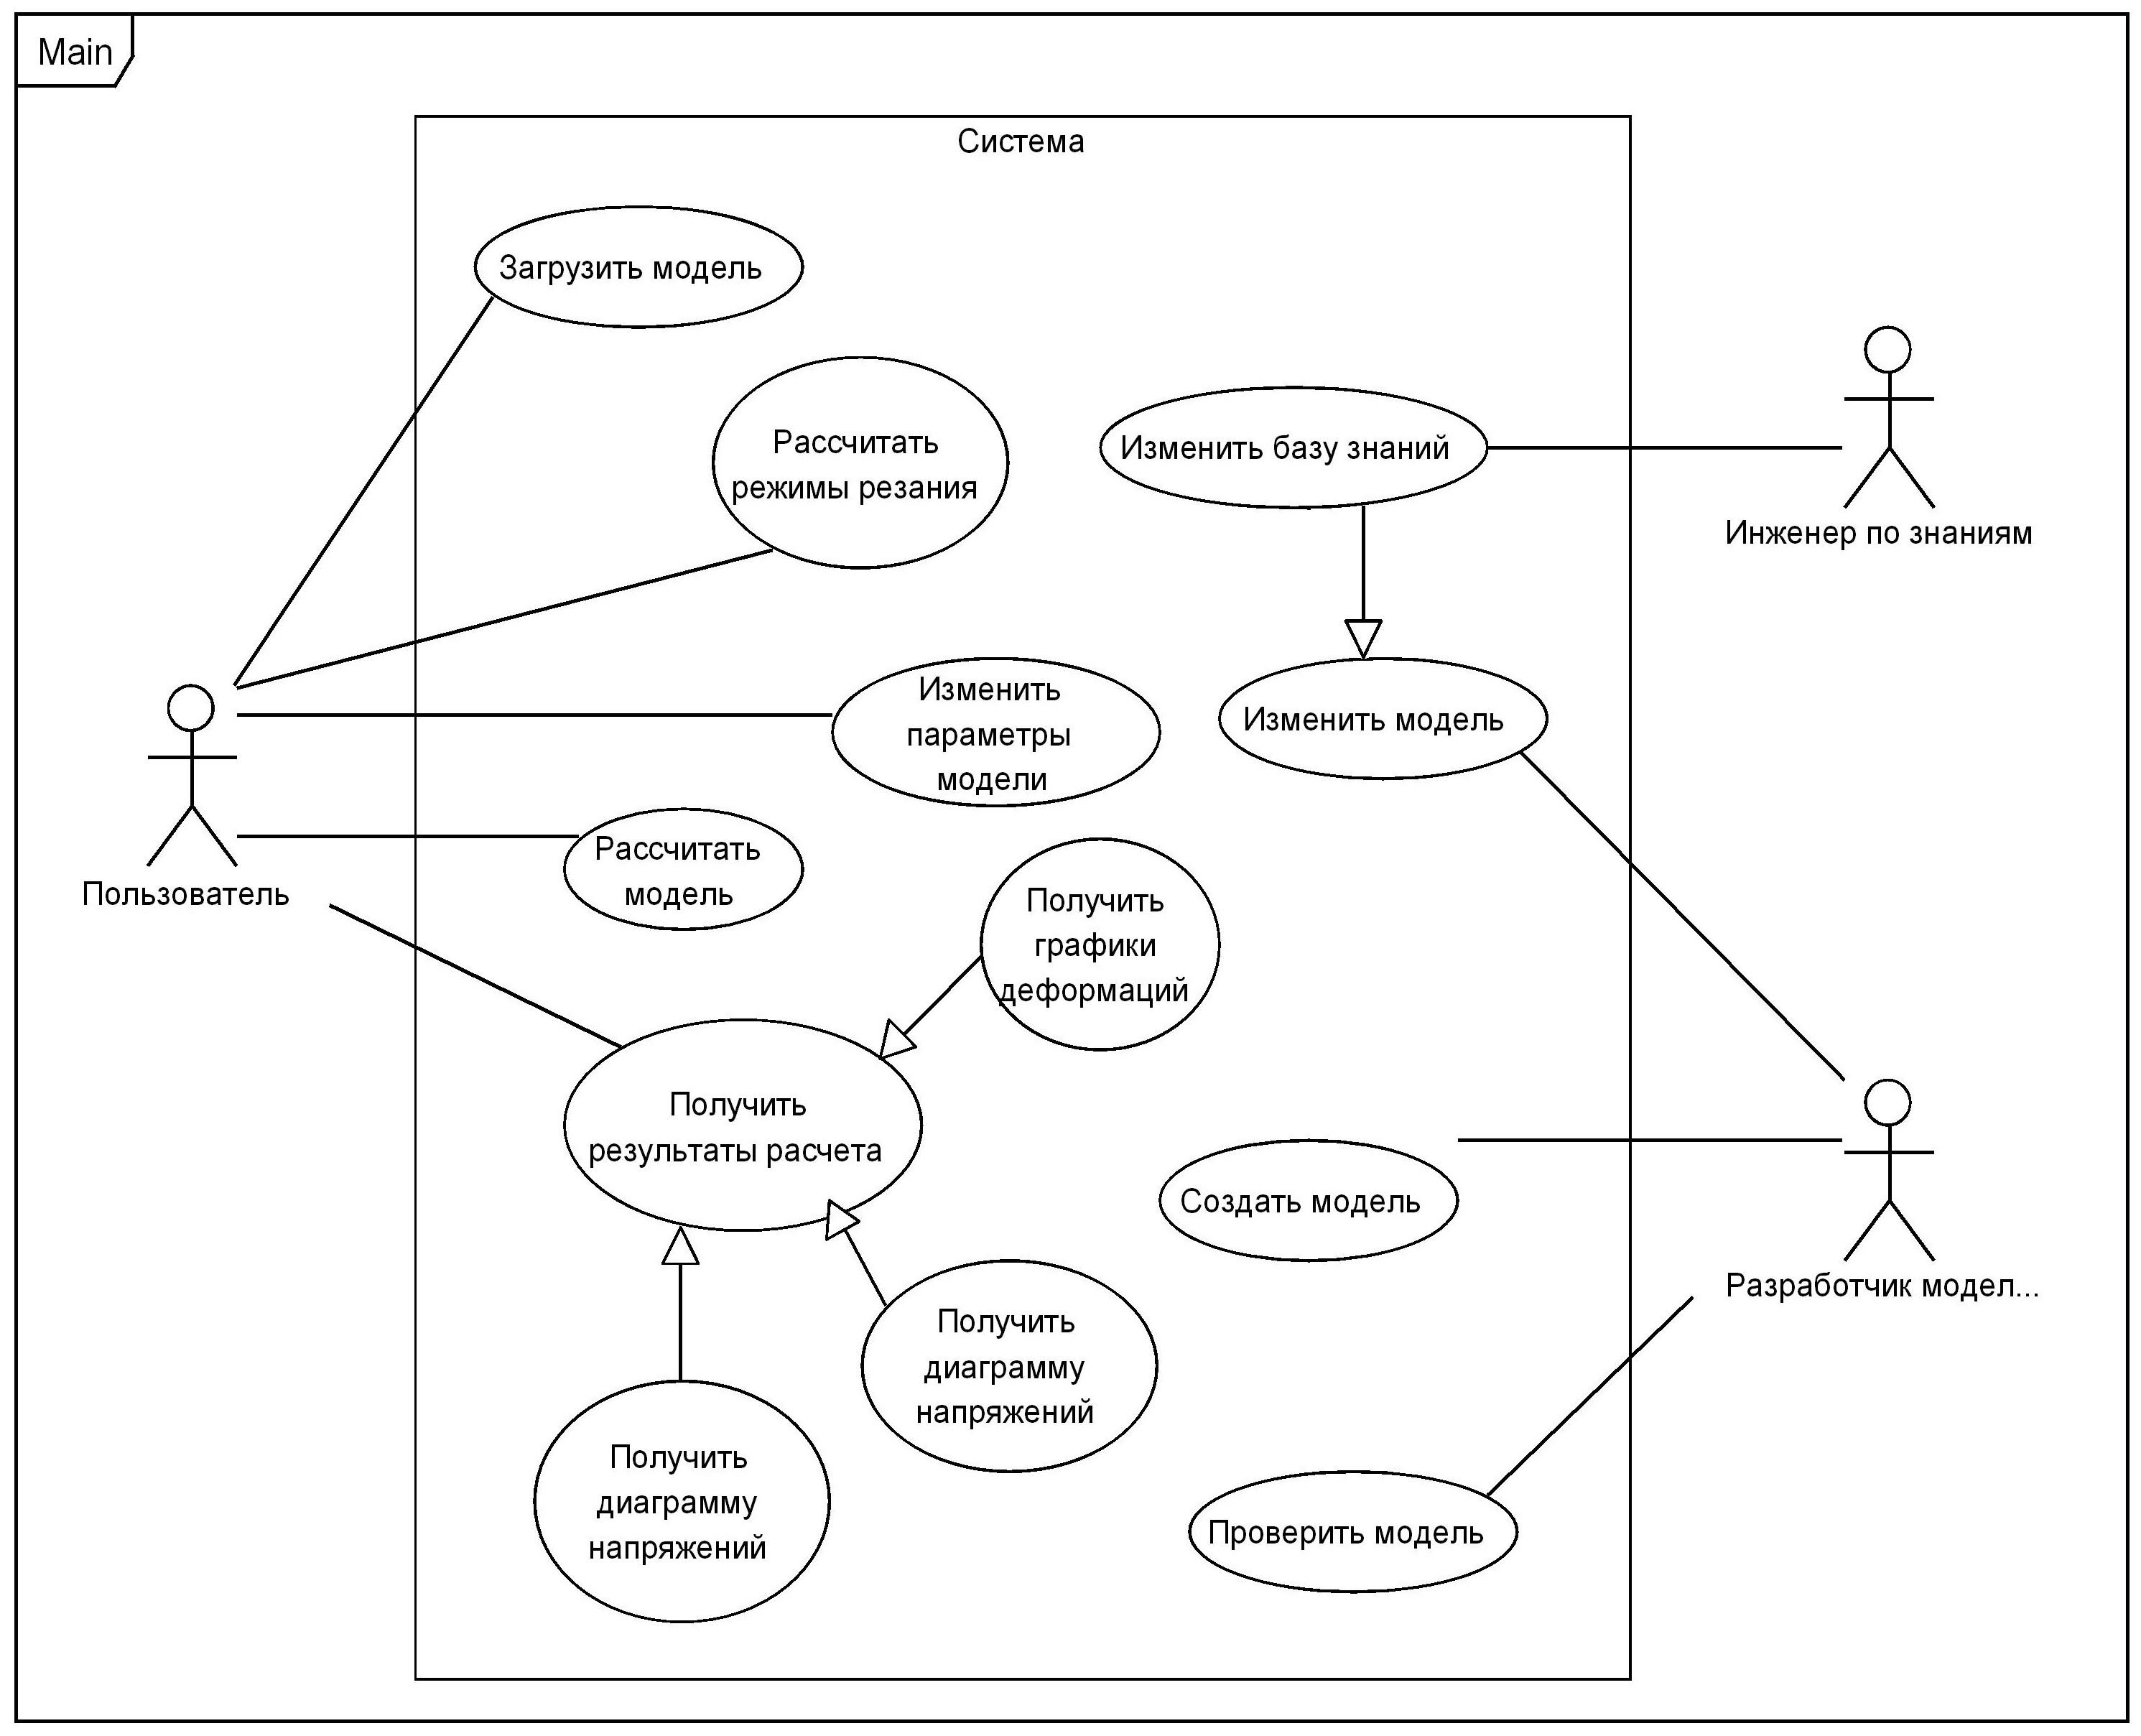
\includegraphics[scale=0.095]{img/ucd} 
		\end{center}
		\caption{Диаграмма вариантов использования}
		\label{fig:ucd}
		\end{figure}
		
	Первое лицо представлено пользователем, который заинтересован в выполнении функций, связанных с получением значений деформаций заготовки и их анализом. Для этого пользователю должна быть предоставлена возможность загрузки описания расчетного случая (то есть модели) в систему. Перед запуском расчета необходимо применить заданные характеристики процесса к параметризованной модели. По результатам работы CAE системы должны быть получены графики и диаграммы деформаций. Также пользователь ожидает от системы выполнения вспомогательных функций, таких как расчет режимов резания. 
	
	Необходимость выделения такого лица как инженер по знаниям обусловлена результатами анализа литературы \cite{book:Kosilova}, который показал, что для расчета режимов резания по таблично-аналитической методике потребуется представление экспертных знаний в формальном виде. Решение этой задачи возлагается на инженера по знаниям, который должен иметь возможность корректировать содержимое базы знаний, первоначально составленной при разработке системы.  

	Загружаемая в систему модель должна быть предварительно подготовлена компетентным экспертом --- разработчиком моделей. К обязанностям разработчика моделей относится также подготовка исходных данных в виде задания для выполнения CAE системой. После подготовки модели эксперт проверяет её работоспособность и при необходимости  устраняет дефекты, после чего предоставляет пользователю. Общая концепция системы предполагает, что все разработанные модели сохраняются в единую базу моделей, которую технолог использует для выбора расчетного случая, наиболее близкого заданному. Технолог не нуждается в самостоятельном программировании моделей, так как имеющийся состав информационной базы позволяет ему использовать готовые с учетом их высокой степени параметризации. 
	
	Составленная диаграмма вариантов использования изображена на рисунке \ref{fig:ucd}. Кроме описанных выше принципов на ней отображены зависимости обобщения между вариантами использования. Например, варианты использования ``Получить диаграмму деформаций'', ``Получить диаграмму напряжений'' и ``Получить графики деформаций'' обобщены в ``Получить результаты расчета''.  Указанная диаграмма будет использована для выделения отдельных элементов системы в модули для последующей проработке. 

	\section{Разработка структуры входных и выходных данных}
	\subsection{Входные данные для анализа деформаций}
	На этапе эскизного проектирования необходимо определить какие входные данные будут использованы для расчета и в каком виде требуется предстать результат работы системы. В контексте разрабатываемой системы моделью будет называться вся совокупность исходных данных, представленная в виде файла определенной структуры. Таким образом в данном разделе описан состав моделей, используемых системой.
	
	Входные данные должны иметь минимум три основных компонента. На рисунке \ref{fig:model-comp-diarg} показаны основные компоненты и один дополнительный -- трехмерная OBJ модель, загружаемая для визуализации расчетного случая. 
		\begin{figure}[!h]
			\begin{center}
				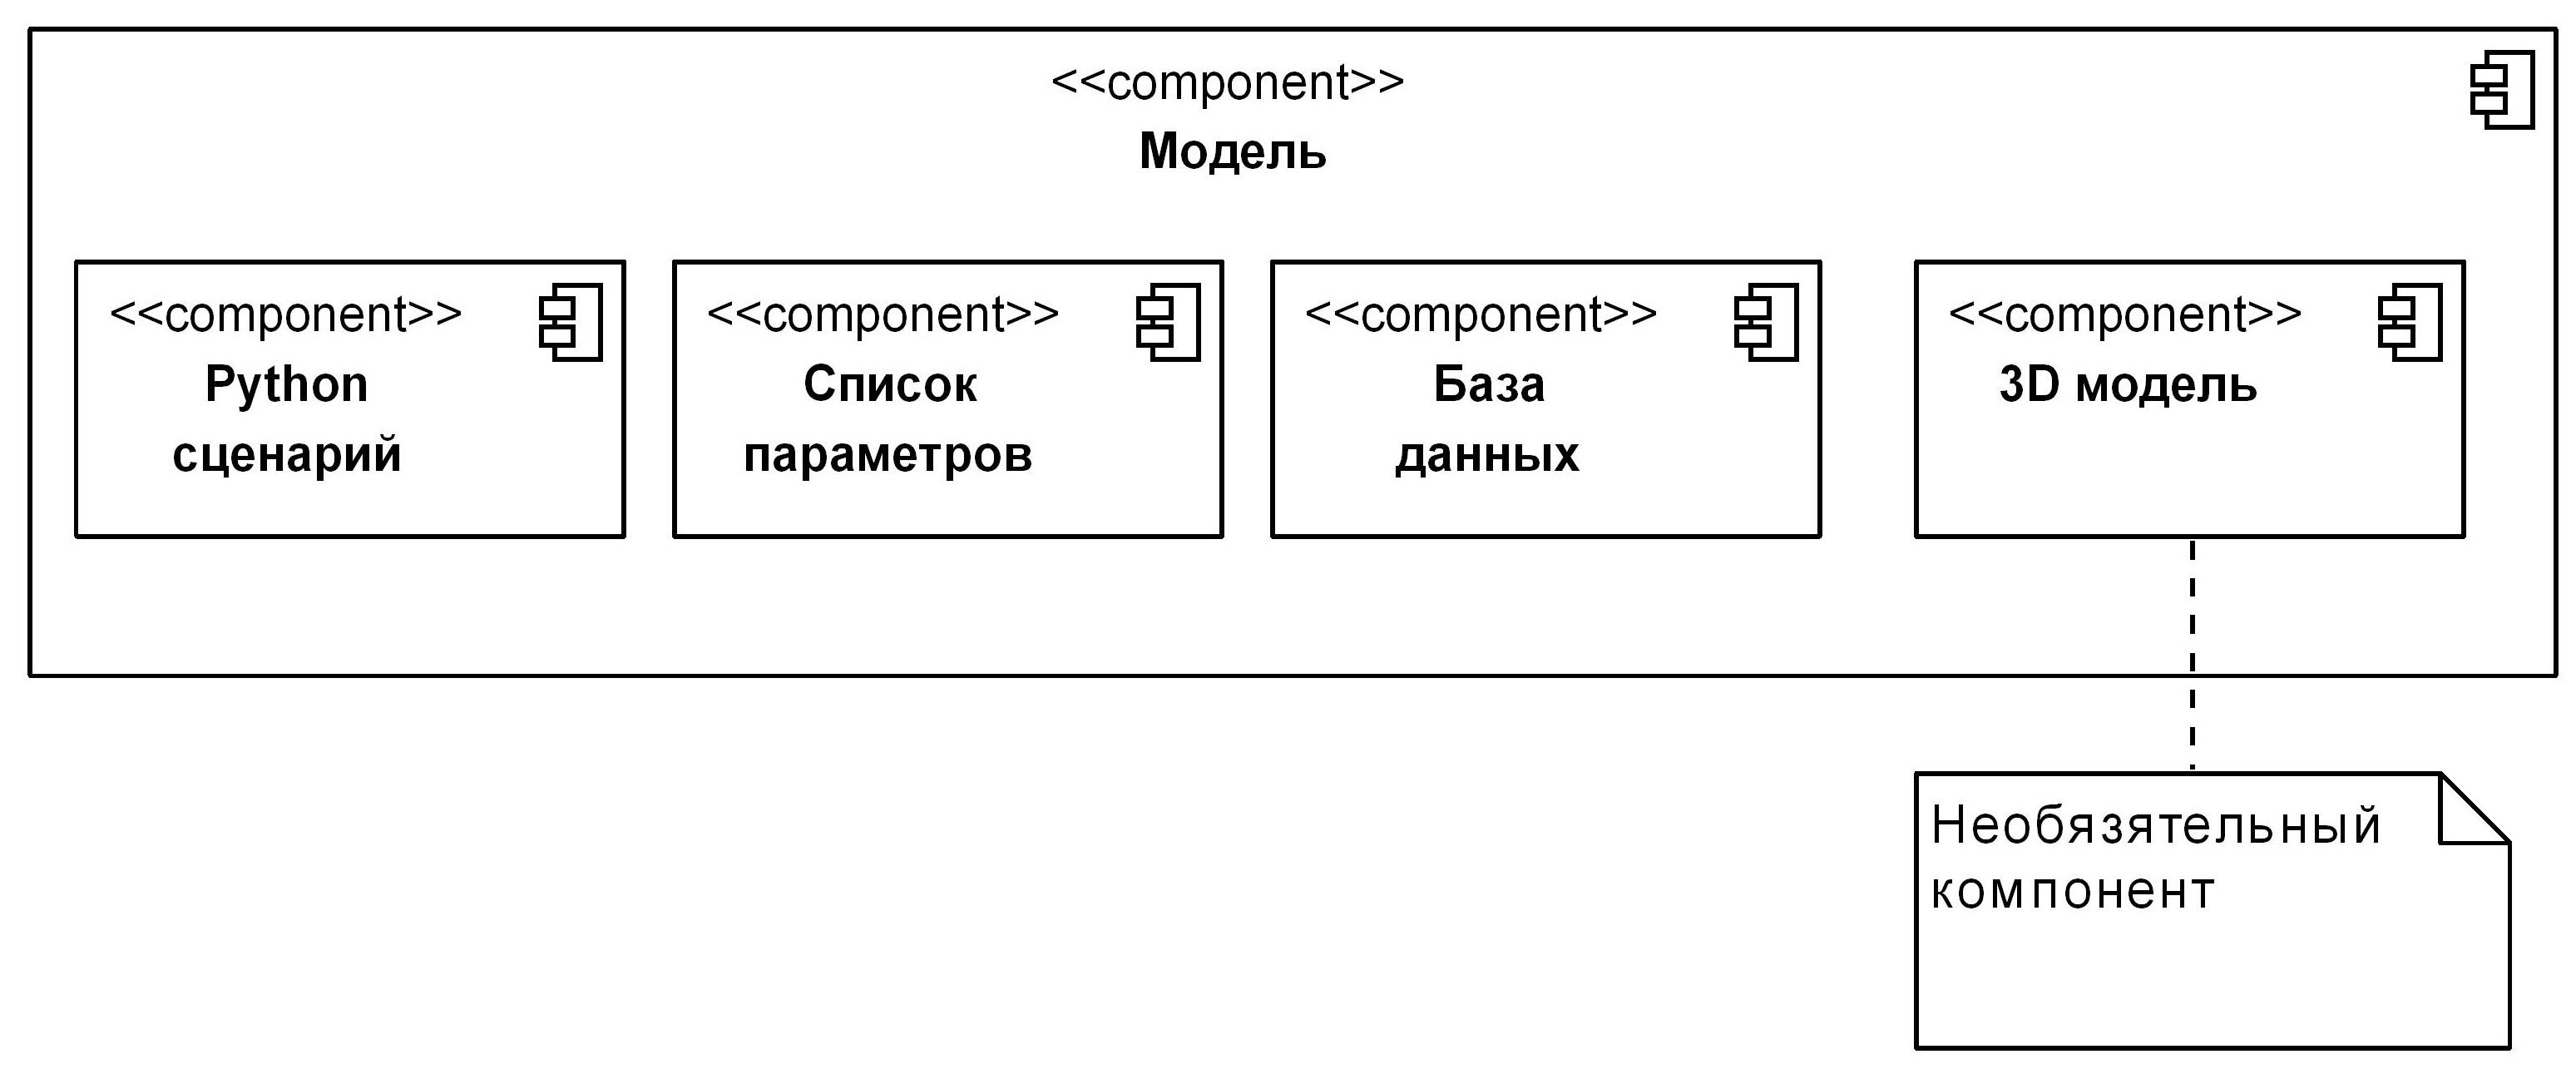
\includegraphics[scale=0.18]{img/model-comp-diarg} 
			\end{center}
			\caption{Компоненты модели}
			\label{fig:model-comp-diarg}
		\end{figure}
	
	Во-первых, сценарий построения расчетного случая в системе Abaqus. CAE система Abaqus, как было указано ранее, использует язык Python для автоматизации расчетов. Выполнение определенной программы позволяет получить поля напряжений и узловых перемещений для запрограммированного сценария, а также записать их в виде графических или текстовых файлов для последующей обработки. Расчетный случай может быть параметризован любым количеством переменных, принимаемых в виде аргументов командной строки при вызове Python скрипта. Таким образом, один сценарий может быть применен многократно для деталей с общей формой, но различными значениями геометрических размеров. 
	
	Python относится к высокоуровневым объектно-ориентированным языкам программирования общего назначения. Он имеет динамическую типизацию, синтаксически простые конструкции ветвления, последовательного перебора элементов коллекций, обработки исключений, что делает его чрезвычайно легким в освоении и при этом гибким и мощным средством автоматизации. 
	
	Вторая составляющая модели -- это список параметров. Все параметры должны быть перечислены в отдельной структуре с указанием комментариев и размерности для того чтобы пользователь мог выбрать и изменить необходимые из них. Эта структура загружается системой вместе с остальными компонентами и отображается графическим интерфейсом.  С точки зрения пользователя удобно иерархическое представление набора переменных, когда каждый параметр относится к какой либо подгруппе, например, ``Кулачек'', которая в свою очередь входит в группу более высокого уровня. На самом верхнем уровне находится корневая группа ``Модель''. Таким образом, список параметров будет логически представлен в виде дерева, внутренними узлами которого являются группы параметров, а листовыми вершинами сами параметры. На рисунке \ref{fig:model-tree-abstract} показано абстрактное представление такого дерева произвольной конфигурации. Группы параметров обозначены латинскими буквами <<G>>, а параметры -- буквами <<P>>.  
	
	\begin{figure}[!h]
		\begin{center}
			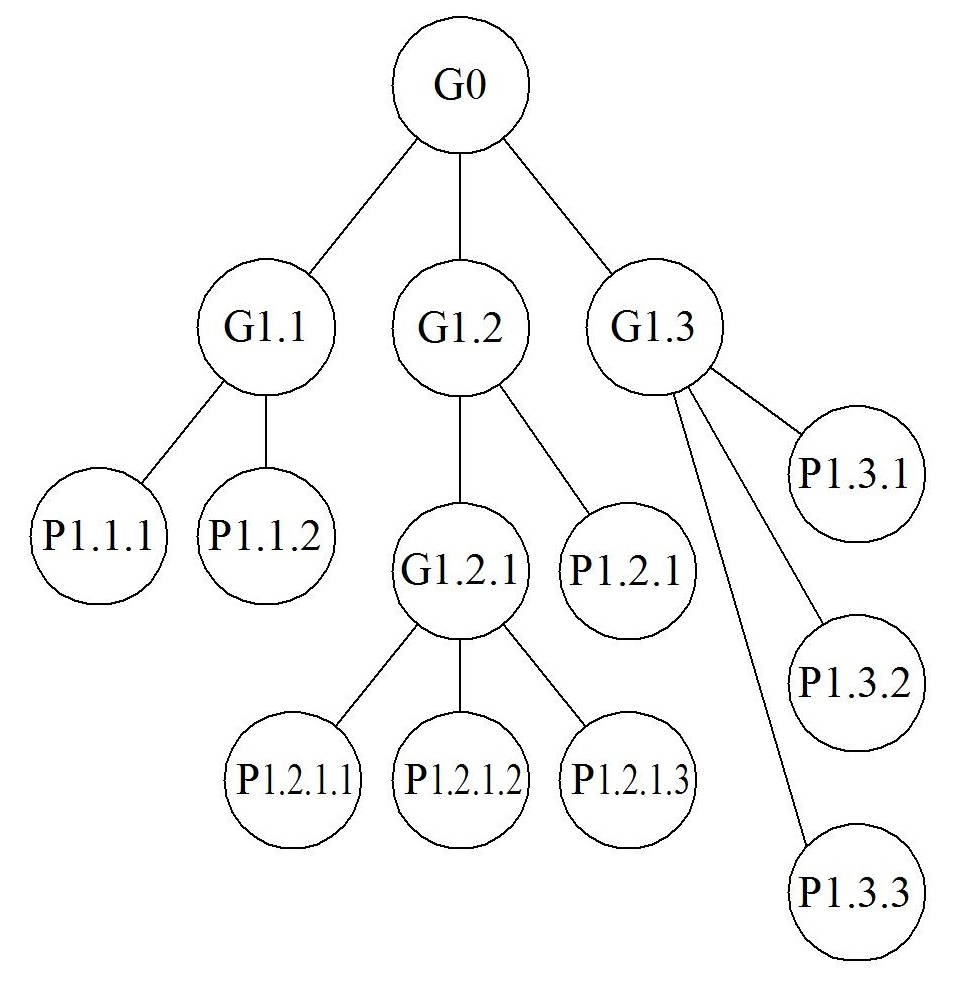
\includegraphics[scale=1]{img/model-tree-abstract} 
		\end{center}
		\caption{Дерево параметров}
		\label{fig:model-tree-abstract}
	\end{figure}
		
	Параметр с точки зрения пользователя представляется как кортеж трех элементов: $ \langle N,C,V \rangle $, где N~--~название параметра (name), например, ``Сила резания'', С~--~комментарий (commentary), поясняющий роль параметра и указывающий его размерность и V~--~значение (value) параметра, которое вводится пользователем.Группы параметров имеют только имя и служат контейнерами, обеспечивающие иерархическую вложенность.  
	
	Третья составляющая модели -- база данных. База данных предназначена для предоставления справочных значений параметров, таких как свойства материалов. Например, пользователю известно, что деталь изготовляется из углеродистой стали определенной марки. Выбор заданного материала, занесенного в базу данных, инициирует автоматическое заполнение сопутствующих параметров: модуля упругости и коэффициента Пуассона. 
	
	Необязательным компонентом выступает трехмерная модель расчетного случая. Эта модель используется системой  для визуализации схемы закрепления детали и её формы. Хотя трехмерное отображение может быть получено после загрузки модели в систему и выполнения программного сценария, тем не менее такой подход увеличит время загрузки и поэтому был признан неприемлемым. Дополнительно к недостаткам генерации изображения после загрузки можно отнести зависимость от установленной CAE системы. Если на ПК пользователя не установлена CAE система, то пользователь не сможет не только произвести расчет (что ожидаемо), но и открыть модель для просмотра.    

	\subsection{Входные данные для калькулятора режимов резания}	
	Калькулятор режимов резания будет реализован отдельным модулем и для него входные данные вводятся отдельно. В соответствии с таблицами, приведенными в \cite{book:Kosilova}, было определено что для вычисления режимов резания по таблично-аналитической методике требуются входные данные, перечисленные в таблице \ref{tab:calc}. В указанной таблице также приведены возможные значения входных данных. 
	\begin{table}[htb]
		\centering
		\caption{Входные данные калькулятора режимов резания}\label{tab:calc} 
		\begin{tabularx}{\textwidth}{|l|Z|}
			\hline Наименование & Значения \\ 
			\hline Диаметр обрабатываемой поверхности & Числовое в мм \\ 			
			\hline Тип точения & Черновое, получистовое, чистовое \\ 
			\hline Вид обработки & Внешнее точение, растачивание, отрезание \\ 			
			\hline Материал заготовки & Сталь, чугун \\ 			
			\hline Вид заготовки & Поковка, отливка, прокат, полуфабрикат без корки \\ 			
			\hline Материал инструмента & Т15К10, Т15Л6, Т30К4, ВК8, ВК6, ВК4, быстрорежущая сталь \\ 		
			\hline Период стойкости резца & 20, 30, 40, 60, 90 мин \\ 			
			\hline Шероховатость поверхности & По ГОСТ 2789-73 \\ 			
			\hline Радиус при вершине резца & Числовое в мм\\ 			
			\hline 
		\end{tabularx}
	\end{table}
	Для модуля калькулятора режимов резания не требуется разработки какой-либо особой структуры данных так как вся информация непосредственно вводится пользователем с клавиатуры или выбирается из выпадающих списков. 
	
	\section{Эскизное описание принципов работы}
%	\subsection{Межсистемное взаимодействие}
	Работа системы поддержки принятия решения основывается на использовании вычислительных возможностей программы Abaqus. Рассмотрим подробнее последовательность взаимодействия пользователя, разрабатываемой системы и Abaqus. 
	
	На рисунке \ref{fig:seq-diagram} приведена UML диаграмма последовательностей. На диаграмме показана последовательность обмена сообщениями для варианта использования ``Изменить параметры модели'' и ``Рассчитать модель'' а также вариант использования ``Обновить модель'', который не показан на диаграмме прецедентов для упрощения восприятия.  

	\begin{figure}[!h]
		\begin{center}
			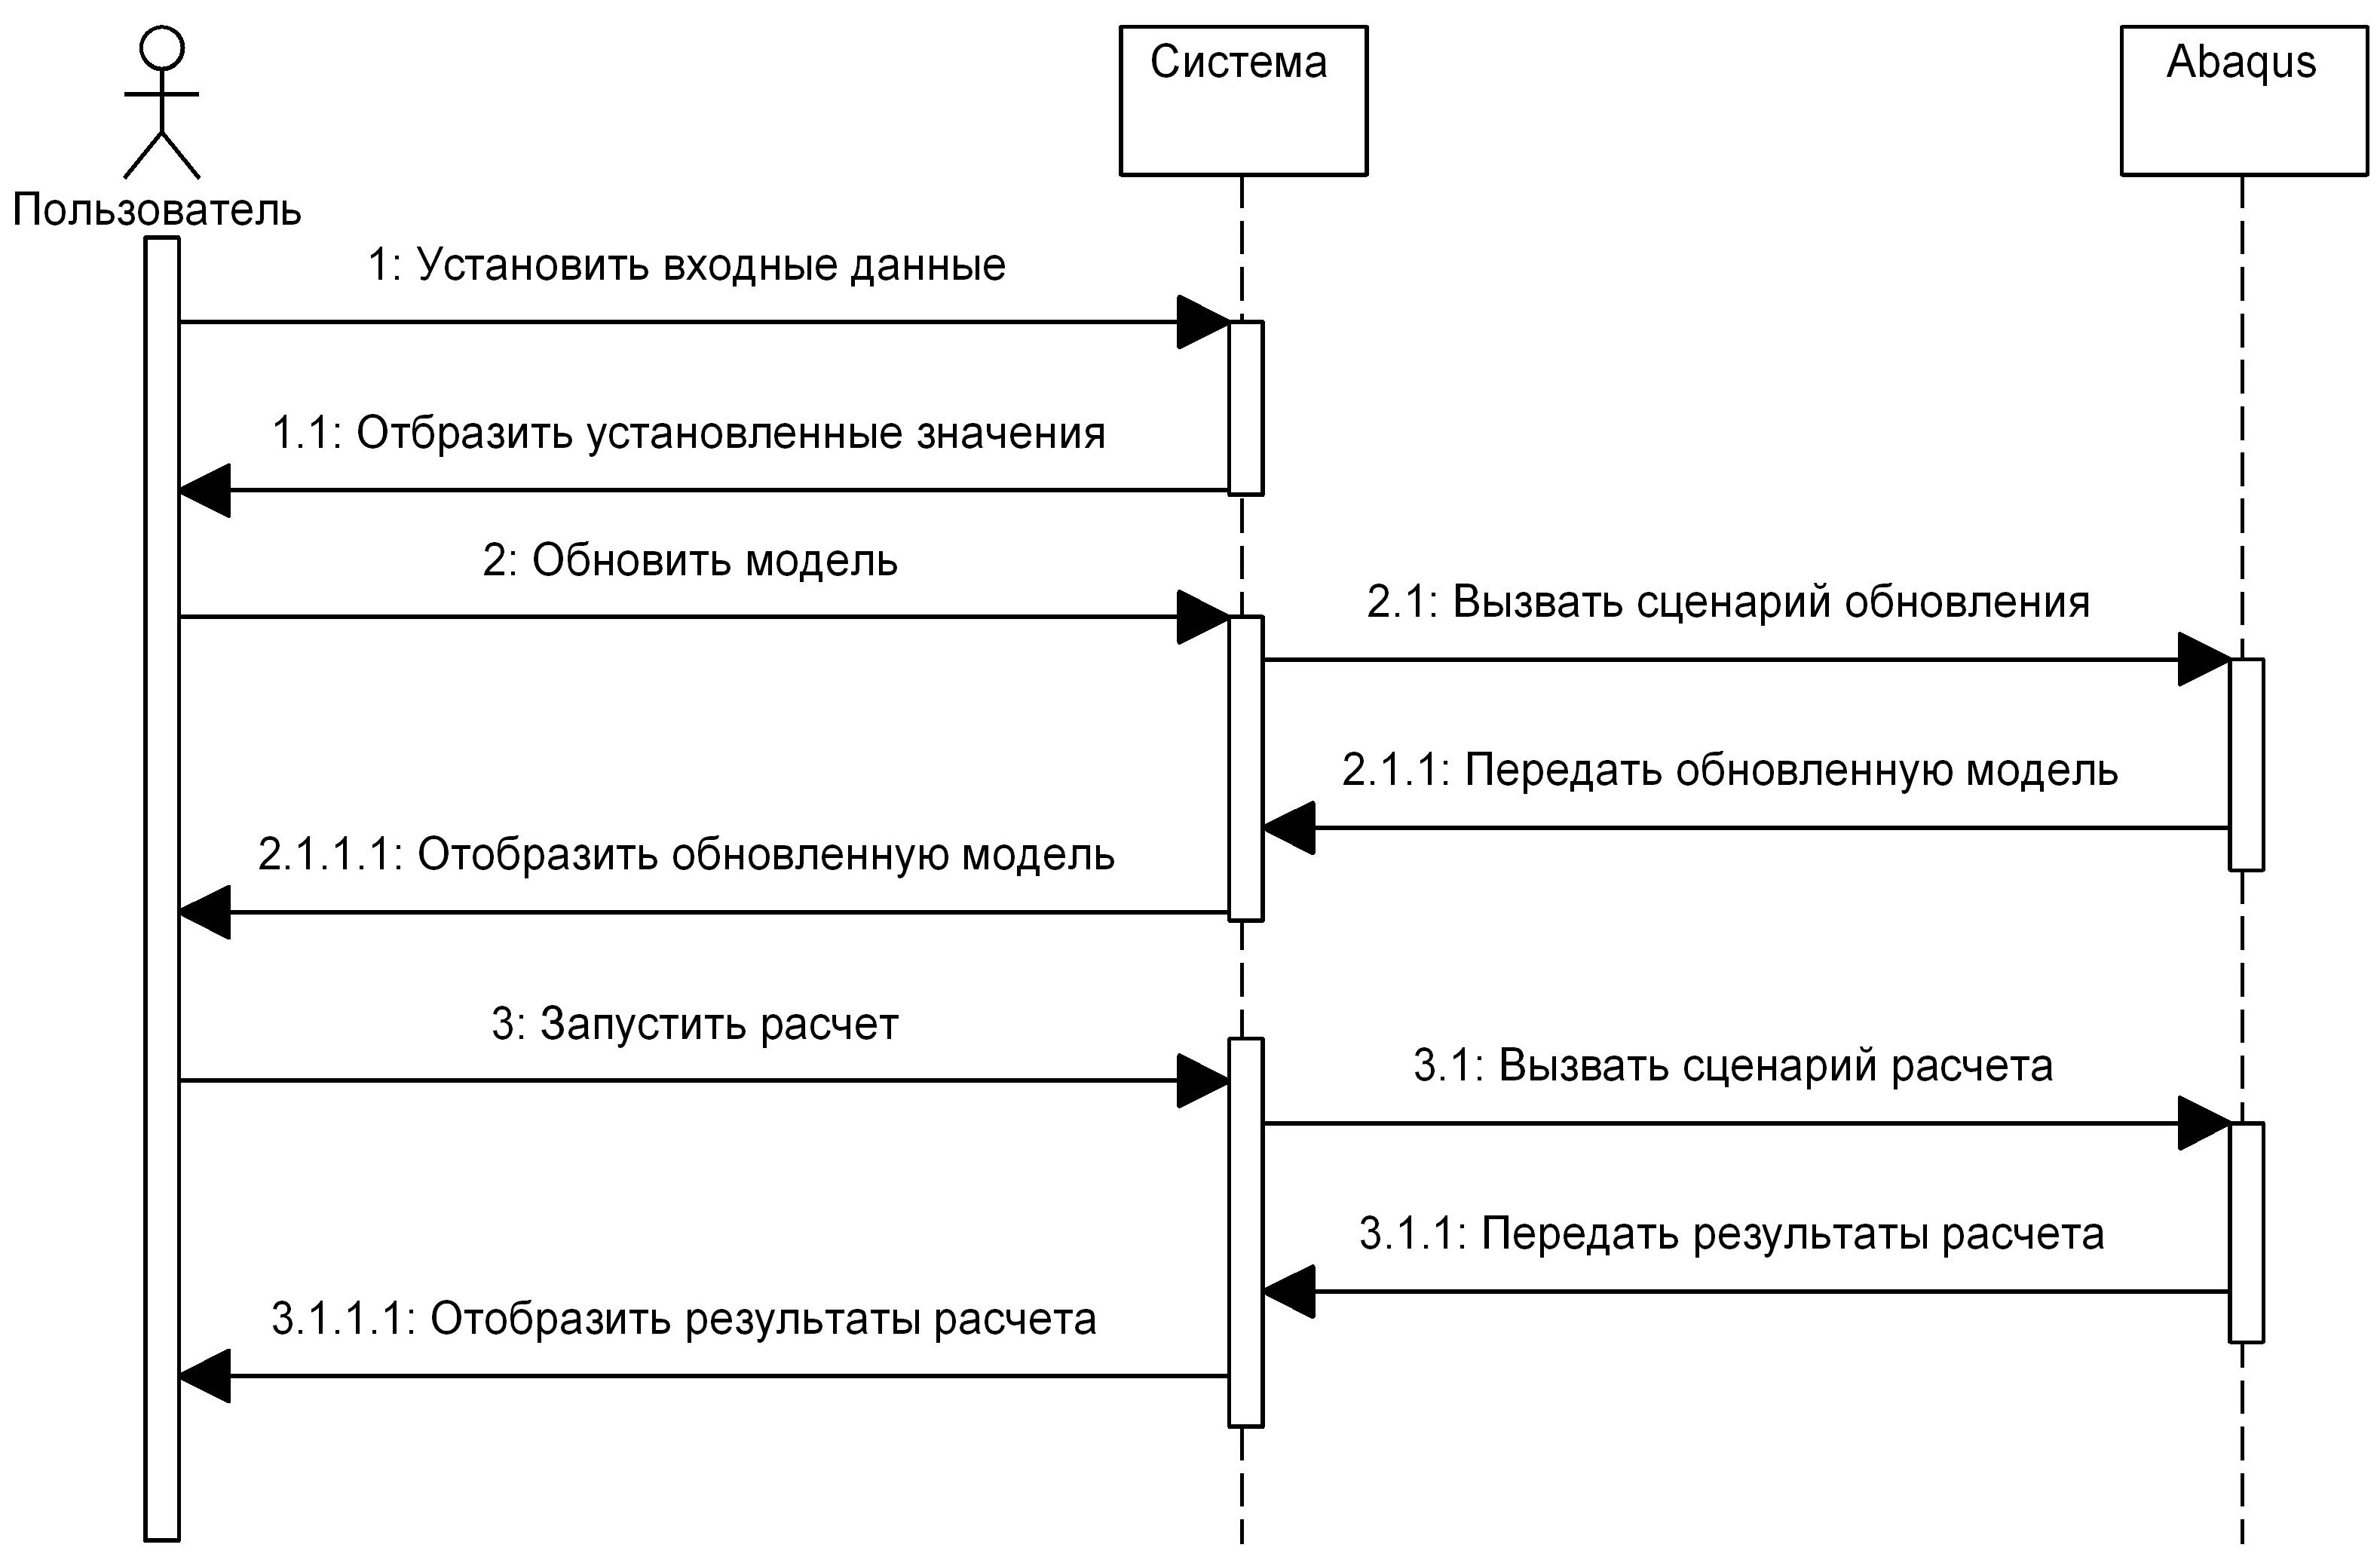
\includegraphics[scale=0.18]{img/sequence-diagram} 
		\end{center}
		\caption{Диаграмма последовательностей}
		\label{fig:seq-diagram}
	\end{figure}	
	
	Как видно из диаграммы, при задании пользователем значений параметров система сохраняет их в оперативной памяти и отображает в графическом интерфейсе. В случае если пользователю требуется обновить трехмерное отображение заготовки, программа обращается к Abaqus, вызывая специальный сценарий обновления, который представляет собой часть расчетного сценария, но вместо запуска вычислений сохраняет перестроенную геометрию в обменный файл, которым пользуется система для визуализации изменений. Аналогичный обмен сообщениями происходит при запуске расчета, но в этом случае уже вызывается полный сценарий, вычисляющий перемещения и напряжения в детали. 
	
	\section{Модули}
	Разрабатываемая программа опирается на использование технологии NetBeans Platform, что позволяет при проектировании оперировать понятием модуля системы. В данном разделе описываются принципиальные подходы используемой технологии и их практическое применение. 
	\subsection{Концепции NetBeans}	
	В основе NetBeans Platform лежит идея, что каждая часть кода приложения принадлежит какому либо модулю \cite{book:NetBeans}. Суть такого подхода заключается в том, что для каждого модуля определена собственная область видимости и коммуникация между модулями осуществляется только по определенным интерфейсам, которые описывают правила взаимодействия, но не раскрывают подробностей его реализации. 
	
	Концепция модуля в NetBeans платформе отличается от концепции Java пакета так как модуль имеет большую независимость от своей среды. Он объединяет несколько логически и функционально связных пакетов, инкапсулируя их. В некоторых случаях модуль может экспортировать внутренний пакет для совместного использования. 
	
	Для передачи объекта от одного модуля к другому предусмотрена концепция поиска (``Lookup'') объектов. Модуль-поставщик публикует объект определенного типа в экземпляр разделяемого класса (то есть класса, доступного обоим модулям), а модуль-приемник на основе механизма прослушивания или при непосредственной проверке в результате поиска объекта заданного типа получает ссылку на передаваемый объект и использует её для своего функционирования.
	
	Таким образом, каждый модуль может быть разработан автономно, при условии соблюдения контрактов, описанных интерфейсами. Модуль должен быть слабо связан с самой системой, иметь лишь необходимый минимум зависимостей и не использовать специфических недокументированных особенностей кода, с которым происходит взаимодействие. В таком случае разработанная система отвечает требованиям простоты обслуживания и может быть легко расширена новыми функциональными возможностями.

	\subsection{Применение платформы}	
	На эскизном этапе проектирования необходимо уточнить состав модулей и их предназначение. Вопросы реализации отдельных компонентов будут рассмотрены при техническом проектировании. В таблице \ref{tab:modules} приведены разрабатываемые модули с указанием краткого описания по каждому из них. Название модуля отражает его предназначение. Первая часть названия ``eremeykin.pete.'' 	одинакова для всех разрабатываемых компонентов и составлена по подобию именования Java пакетов. Если название содержит в себе сокращение ``api'', то такой модуль используется внешними модулями и предназначен для описания интерфейсов взаимодействия. 
		\begin{longtable}{| p{.40\textwidth} | p{.55\textwidth} |}
			\caption{Состав модулей}\label{tab:modules} \\
			\hline Полное название & Предназначение \\ 
			\hline eremeykin.pete.api.core & Обмен объектами между модулями, обработка запуска системы и управление директориями рабочего пространства \\ 
			\hline eremeykin.pete.api.executor & Описание интерфейса вызова внешней CAE системы \\ 
			\hline eremeykin.pete.api.model & Определение классов модели и параметра для совместного использования другими модулями\\ 
			\hline eremeykin.pete.actions & Делегирование соответствующим компонентам возможных действий пользователя, таких как ``Обновить модель'' и ``Расчитать модель'' \\ 
			\hline eremeykin.pete.calculator & Обеспечение функционала калькулятора режимов резания \\ 
			\hline eremeykin.pete.editor & Редактирование значений параметров модели  \\ 
			\hline eremeykin.pete.launcher.abaqus & Конкретная реализация исполнителя Abaqus сценариев \\ 
			\hline eremeykin.pete.loader & Загрузка моделей в систему\\ 
			\hline eremeykin.pete.logger & Отладочные средства, логирование\\ 			
			\hline eremeykin.pete.plotter & Загрузка результирующих данных и построение графиков деформаций \\ 			
			\hline eremeykin.pete.reports & Генерация отчетных документов\\ 			
			\hline eremeykin.pete.viewport & Трехмерное отображение модели детали \\ 			
			\hline 
		\end{longtable}

	Для организации слабосвязанной системы модулей было выделено три компонента, которые  экспортируют один или несколько пакетов, позволяя тем самым ввести общие для всей системы соглашения. Например, основополагающим понятием является модель. Класс модели должен быть использован во многих модулях, таких как модуль редактора параметров eremeykin.pete.editor или загрузчик eremeykin.pete.loader.  
	
	\chapter{Техническое проектирование}
	\section{Уточнение структуры входных данных}
	Ранее было определено, что исходные данные загружаются в систему в виде модели, содержащей всю необходимую информацию для работы системы. Определим подробнее формат хранения этой информации и способы её извлечения. 
	
	По результатам эскизного проектирования установлено, что большая часть информации должна быть сохранена в табличном виде. Между определенными фрагментами данных существуют логические связи, например, между названием материала заготовки и его физическими свойствами. Таким образом, было принято решение  использовать базу данных (БД) как источник информации о загружаемой модели. 
		
	\begin{figure}[h!]
		\begin{center}
			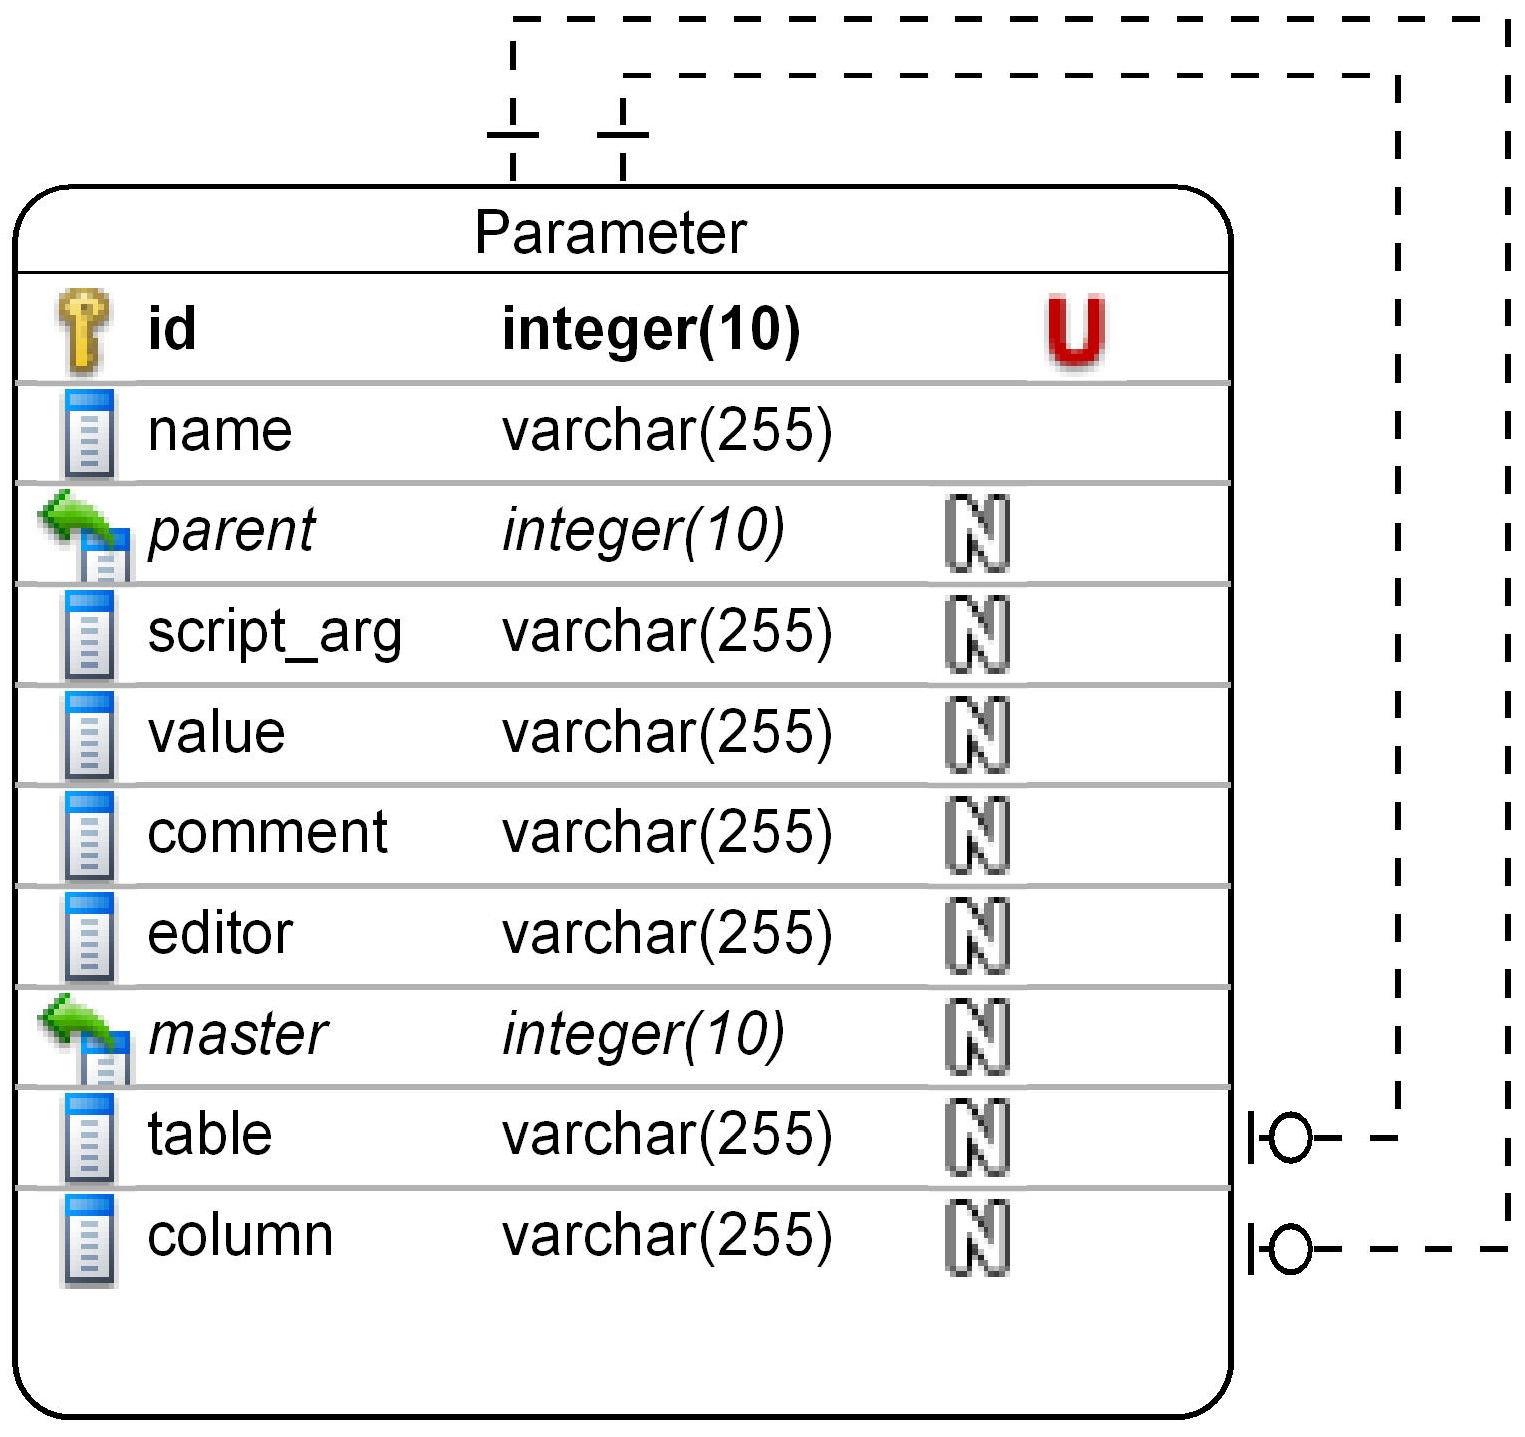
\includegraphics[scale=0.2]{img/ER-diagram} 
		\end{center}
		\caption{ER диаграмма}
		\label{fig:er-diagram}
	\end{figure}
		
	В качестве альтернативного варианта реализовано хранение моделей в табличном файле Excel. Этот способ существенно проще с точки зрения пользователя и разработчика моделей так как данные могут быть отредактированы в графическом интерфейсе Microsoft Office или аналогичных программ. Табличная структура файлов Excel в целом похожа на способ представления данных в БД, поэтому будет разработан один способ записи модели для двух вариантов физической реализации.
	
	На рисунке \ref{fig:er-diagram} изображена ER диаграмма, показывающая состав атрибутов параметров модели и их отношения. Параметр имеет 10 атрибутов в общем случае, некоторые из которых могут иметь значение \texttt{NULL} (помечены буквой N). Группы параметров, о которых было сказано на этапе эскизного проектирования, также описываются сущностью \texttt{Parameter}, но имеют определенные особенности. 
	
	Атрибут \texttt{id} выступает в роли первичного ключа и имеет целочисленное уникальное значение (помечено буквой U). Он не отображается в пользовательском интерфейсе программы и необходим для построения древовидной структуры с помощью ссылок. 
	
	За отображение названия параметра в графическом интерфейсе отвечает атрибут \texttt{name}, имеющий строковое значение. Название кратко характеризует роль параметра в модели. Примерами имени являются ``Модуль упругости'',  ``Ширина'' для параметров, а для групп~--~``Кулачки'', ``Деталь''. Для данного атрибута не допускается указывать \texttt{NULL} значение, так как параметр или группа обязательно должны иметь название.

	Особую роль в построении иерархии параметров играет атрибут \texttt{parent}. Этот атрибут указывает на своего родителя более высокого уровня. Родителем параметра может выступать только группа параметров, как показано на рисунке \ref{fig:model-tree-abstract}. Например, на этом рисунке параметр P1.1.1 входит в состав группы G1.1. Тогда значение \texttt{parent} для этого параметра будет содержать \texttt{id} группы G1.1. Аналогично для групп нижних уровней в роли родителя выступает группа верхнего уровня. Корневая группа имеет значение \texttt{parent=NULL}, что допустимо согласно приведенной ER диаграмме. Для приведенного на рисунке \ref{fig:model-tree-abstract} примера составлена таблица \ref{tab:model-tree-abstract}.
		
	\begin{figure}
		\centering	
		\noindent\begin{minipage}{0.5\textwidth}% adapt widths of minipages to your needs
			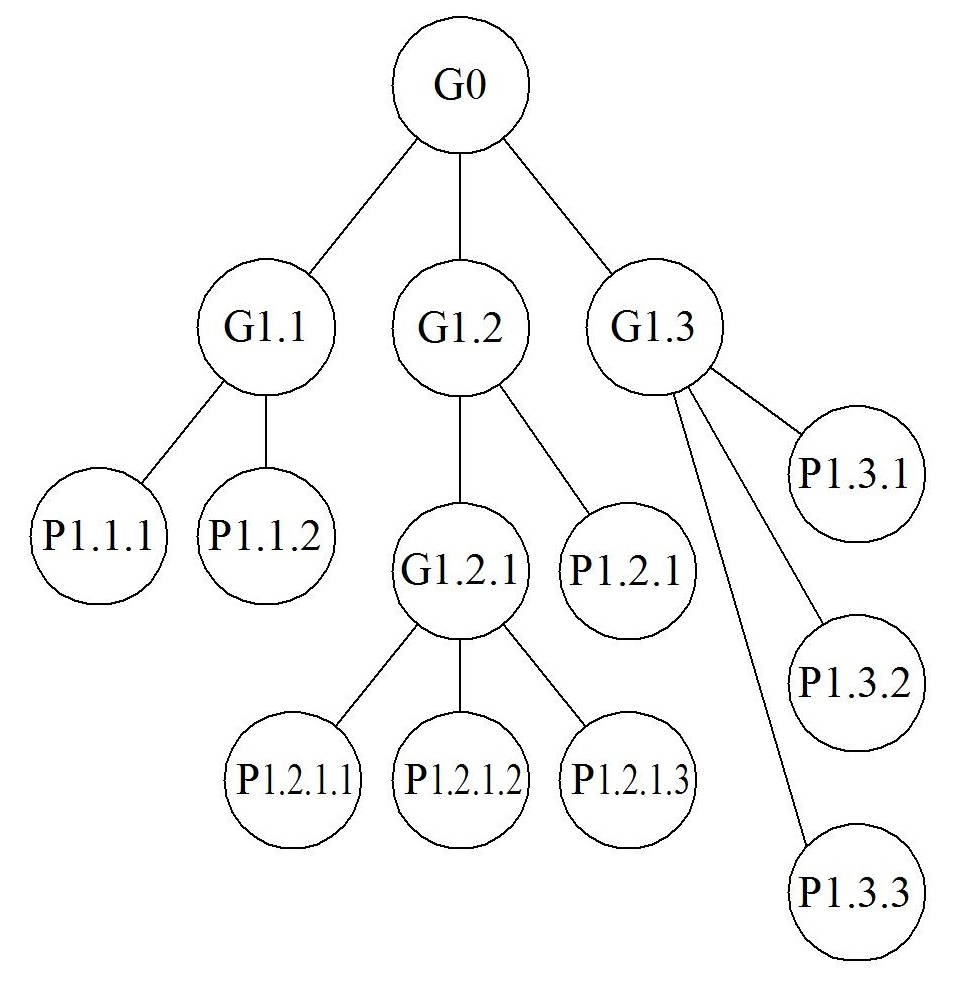
\includegraphics[scale=1]{img/model-tree-abstract} 
			\hfill%
		\end{minipage}%
		\begin{minipage}[b]{0.4\textwidth}
				\centering
				\captionof{table}{}
				\label{tab:model-tree-abstract}			  			
				\begin{tabularx}{\textwidth}{|c|Z|Z|} 
					\hline id & name & parent\\ 
					\hline 0 & G0 & NULL\\ 
					\hline 1 & G1.1 & 0\\ 			
					\hline 2 & G1.2 & 0\\ 
					\hline 3 & G1.3 & 0\\ 			
					\hline 4 & P1.1.1 & 1\\ 			
					\hline 5 & P1.1.2 & 1\\ 			
					\hline 6 & G1.2.1 & 2\\ 			
					\hline 7 & P1.2.1 & 2\\ 						
					\hline 8 & P1.3.1 & 3\\ 			
					\hline 9 & P1.3.2 & 3\\ 
					\hline 10 & P1.3.3 & 3\\ 
					\hline ... & ... & ...\\ 				
					\hline 
				\end{tabularx}
		\end{minipage}
	\end{figure}
	
	Для передачи действительных значений параметров в Python скрипт используется атрибут \texttt{script\_arg}, который указывает принадлежность конкретного значения к определенному параметру. Пример команды, вызывающей запуск скрипта можно записать следующим образом: \begin{verbatim}abaqus cae noGUI=script.py inner=0.028 outer=0.03 ... \end{verbatim}	
	Из примера видно, что для ассоциации значения параметра используются ключевые слова, такие как \texttt{inner} и \texttt{outer} с помощью которых скрипт распознает за что отвечает следующее за символом ``\texttt{=}'' значение. Эти ключевые слова записываются в колонке  \texttt{script\_arg}. Значение \texttt{NULL} служит для обозначения групп параметров или каких-либо отдельных вспомогательных параметров, значение которых не требуется для работы Python скрипта.

	Атрибут \texttt{value} служит для выставления значения по-умолчанию и может быть впоследствии использован при сохранении состояния модели в файл. Этот атрибут выводится на экран после загрузки модели и изменяется пользователем в графическом интерфейсе. Для групп и параметров, не требующих значения по-умолчанию, \texttt{value} устанавливается равным \texttt{NULL}. 

	Для вспомогательных пояснений относительно роли конкретного параметра предусмотрен атрибут \texttt{comment}. Как следует из названия в нем хранятся строковые комментарии. Хорошей практикой считается указание размерности в этой графе помимо дополнительной информации. Есть возможность не использовать комментарии, если в них нет необходимости. При этом атрибут  \texttt{comment} принимает значение \texttt{NULL}. 
	
	Колонка \texttt{editor} описывает тип редактируемого параметра. Если параметр не может быть изменен пользователем, то в поле \texttt{editor} записывается \texttt{NULL}, это же значение присваивается группам параметров. Для редактируемых параметров предусмотрено 3 допустимых значения: \texttt{text}, \texttt{auto} и \texttt{cbox}. Значение \texttt{text} соответствует простому текстовому полю для ввода числового или строкового значения. Например, такое поле используется для описания параметра ``Внешний радиус''. Если указано значение \texttt{auto}, то в этом случае величина параметра должна быть определена автоматически в зависимости от другого параметра. Примером автоматически заполняемого параметра является ``Модуль упругости''. Для обозначения параметра, редактируемого выпадающим списком с предлагаемым набором значений служит \texttt{cbox}.

	Принимая во внимание зависимость некоторых параметров от других (например, модуль упругости зависит от материала), было принято решение отмечать такую зависимость в таблице параметров при помощи атрибута \texttt{master}. Этот атрибут указывает на \texttt{id} главного параметра, который управляет текущим. То есть если в поле \texttt{master} параметра ``Модуль упругости'' будет указан \texttt{id} параметра ``Название материала'', то модуль упругости будет выставляться в зависимости от выбранного материала. Но для этого необходимо сопоставить название материала и его параметры. Эту роль выполняет дополнительная таблица \texttt{materials}. Для указания таблицы соответствия (в роли неё могут выступать и другие таблицы, не обязательно \texttt{materials} ) используется атрибут \texttt{table}, а атрибут \texttt{column} указывает на колонку по которой выбирается значение. 
	
	\begin{comment}
	Фрагмент записи модели приведен в таблице \ref{tab:model}. 
	\begin{table}[htb]
		\small
		\centering
		\caption{Фрагмент модели}\label{tab:model} 
		\begin{tabularx}{\textwidth}{|c|c|c|c|c|c|c|c|c|Z|}
			\hline id & name & parent & script\_arg &	value & comment & editor &	master &	table &	col \\ 			
			\hline 5 & Материал & 1 &  &  &	Материал &  & &  &  \\ 
			\hline 6 & Название & 5 &  & &	Название & cbox &  & materials & name \\ 			
			\hline 
		\end{tabularx}
	\end{table}
	\end{comment}
	
	\section{Чтение входных данных}
	Входные данные могут быть извлечены из SQL базы данных или из Excel таблиц. При разработке способа их чтения следует предусмотреть и другие варианты хранения на случай расширения системы, поэтому чтение входных данных рассмотрено подробно. 
	
	\subsection{Подключение базы данных}
	Для извлечения информации из баз данных при помощи языка Java существует стандартный способ, называемый Java Data Base Connectivity (JDBC). Последняя версия JDBC 4.2 описывается в документе Java Specification Request (JSR) 221. 
	
	Преимущество этого стандарта заключается в том, что при условии рационального программирования SQL запросов, он позволяет создать программу, не зависящую от конкретной реализации системы управления базами данных (СУБД). Стандарт JDBC основывается на использовании так называемых JDBC драйверов. Каждый производитель, поддерживающий работу со своими СУБД поставляет как минимум один драйвер, который, согласно стандарту, содержит определенную реализацию интерфейса java.sql.Driver. Таким образом достигается отсутствие непосредственной связи кода программы и кода JDBC драйверов различных производителей СУБД. Например, если изначально программа была ориентирована на использование СУБД Oracle Database и при этом не были задействованы особенности диалекта Oracle SQL, то в процессе последующего развития к программе могут быть подключены и другие системы управления базами данных (например, MySQL), что потребует добавления соответствующего JDBC драйвера. 
	
	\subsection{Выбор СУБД}
	Определим СУБД которая будет использована на начальных стадиях развития интегрированной системы поддержки принятия решений. Так как на момент разработки ещё не существует соответствующей информационной среды, то будет использована встраиваемая СУБД, работающая на том же компьютере что и сама система. При последующем развитии системы встраиваемая СУБД может быть заменена на клиент-серверную, так как механизм JDBC взаимодействия остается общим. 
	
	Простота, удобство и функциональность определили выбор SQLite. СУБД относится к встраиваемым так как не требует запуска отдельного серверного процесса, а подключается в виде библиотеки. Все данные сохраняются в отдельный файл, который удобно передавать для использования на других компьютерах без необходимости настраивать подключение к серверу, как в случае клиент-серверных СУБД. Тем не менее сохраняются все преимущества реляционных баз данных. 
	
	\subsection{Реализация шаблона DAO}
	В программировании существуют общепринятые методики решения определенных типичных проблем. Эти решения описываются в виде шаблонов проектирования. Благодаря применению шаблонных решений можно существенно снизить трудоемкость создания программных продуктов и повысить эффективность их обслуживания. 
	
	Для решения проблемы чтения данных рекомендуется \cite{web:J2EEPatterns} использовать шаблон Data Access Object (DAO). Этот шаблон подразумевает  введение специального объекта доступа к данным для абстракции и инкапсуляции механизмов взаимодействия с источником информации. Благодаря унификации интерфейса доступа к различным хранилищами достигается большая гибкость архитектуры приложения. В случае, если потребуется реализовать извлечение данных из некоторого нового источника, не предусмотренного изначально техническим заданием, такой функционал можно обеспечить добавлением одного соответствующего класса, при этом не придётся изменять уже написанный код.   
	
	Реализация шаблона DAO включает  четыре компонента. Первый компонент -- объект, которому требуется обеспечить доступ к некоторым данным. Такой объект называют клиентом или бизнес объектом. Второй компонент представляет собой собственно объект доступа к данным (DAO). Он играет роль универсального адаптера, задача которого состоит в скрытии структуры любого хранилища данных, к которому требуется подключиться и предоставлении универсального интерфейса доступа клиента к содержащейся в хранилище информации. Носителем данных выступает третий компонент, представленный в виде класса, экземпляр которого возвращается клиенту. Последним компонентом является  сам источник данных.  
	
	\begin{figure}[!h]
		\begin{center}
			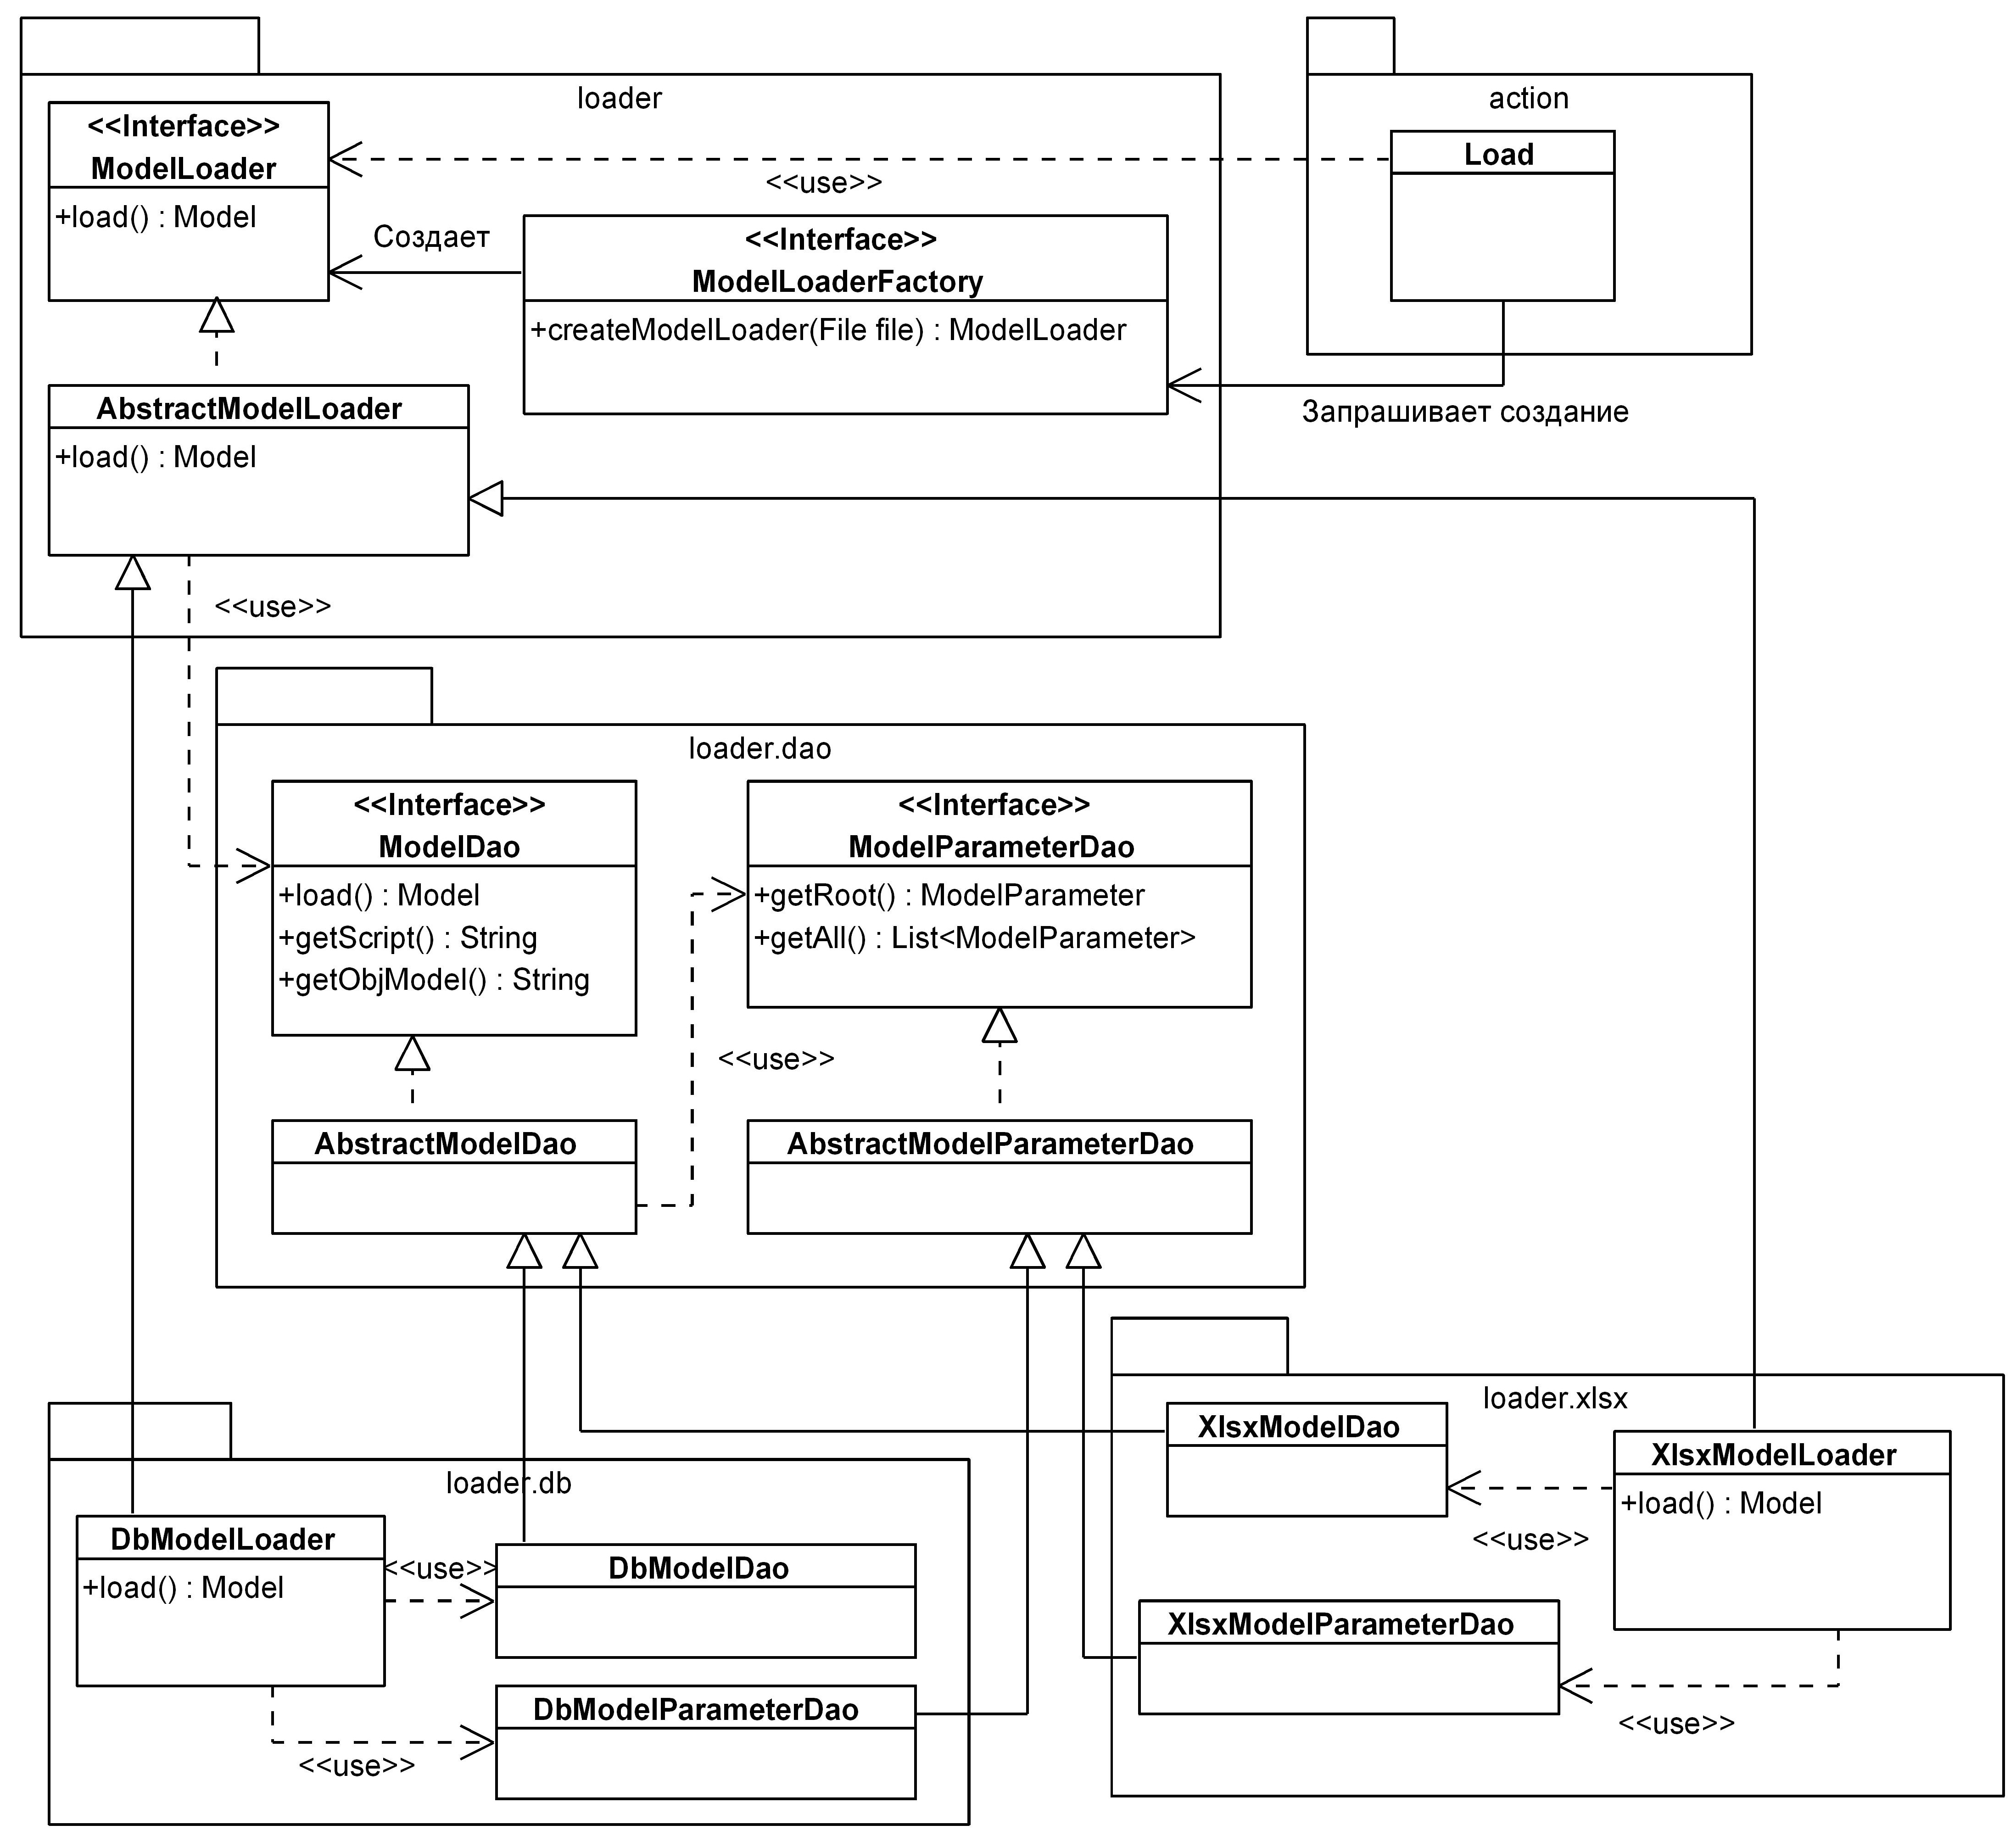
\includegraphics[scale=0.15]{img/class-diagram} 
		\end{center}
		\caption{Диаграмма классов}
		\label{fig:class-diagram}
	\end{figure}
	
	
	В случае интегрированной системы поддержки принятия решений необходимо осуществить чтение информации из SQL базы данных и из Excel файла. Для этого была разработана структура классов, показанная на рисунке \ref{fig:class-diagram}.
	
	В качестве клиента выступает класс, описывающий действия при нажатии на кнопку ``Загрузить модель''. Этот класс назван Load, он реализует интерфейс \texttt{java.awt.event.ActionListener}, объявленный в JDK. Вызовом метода \texttt{createModelLoader(File file)} класс Load запрашивает создание экземпляра \texttt{ModelLoader}. В зависимости от типа файла (.sqlite или .xlsx) клиенту предоставляется та или иная реализация \texttt{AbstractModelLoader} через ссылку типа \texttt{ModelLoader}. Конкретный класс возвращаемого объекта не играет роли для клиента, так как известно, что любая реализация интерфейса \texttt{ModelLoader} имеет метод \texttt{load()}, возвращающий объект модели \texttt{Model}. Именно этот объект и требуется для работы клиента и отображения загруженной модели. 
	
	Имеются две реализации абстрактного класса \texttt{AbstractModelLoader} в соответствии с требуемыми типами хранилищ -- это \texttt{DbModelLoader} и \texttt{XlsxModelLoader}. Первая реализация используется для чтения информации из базы данных и использует JDBC драйвер для выполнения SQL запросов. Вторая реализация считывает данные из xlsx файла при помощи библиотеки Apache POI. 
	
	Собственно объект доступа к данным имеет тип \texttt{ModelDao} для чтения всей модели и \texttt{ModelParameterDao} для чтения отдельного параметра из модели. \texttt{ModelDao} и \texttt{ModelParameterDao} являются интерфейсами, а общая функциональность для всех видов хранилищ вынесена в абстрактные классы \texttt{AbstractModelDao} и \texttt{AbstractModelParameterDao}.  
	
	Благодаря применению шаблона DAO достигается возможность наращивания функционала программы. Например, в данную структуру классов легко добавить возможность загрузки модели из xml файла. Для этого потребуется написать класс \texttt{XmlModelLoader} и соответствующие DAO классы, которые расширяют имеющиеся абстрактные классы. 
	
	\section{Построение МКЭ модели}
	Для демонстрации работоспособности системы будет построена модель обработки тонкостенного цилиндра.  Эскиз детали изображен на рисунке \ref{fig:sketch}, а операционный эскиз на рисунке \ref{fig:oper-sketch} .
	
	\begin{figure}[!h]
		\centering
		\begin{minipage}{.5\textwidth}
			\centering
			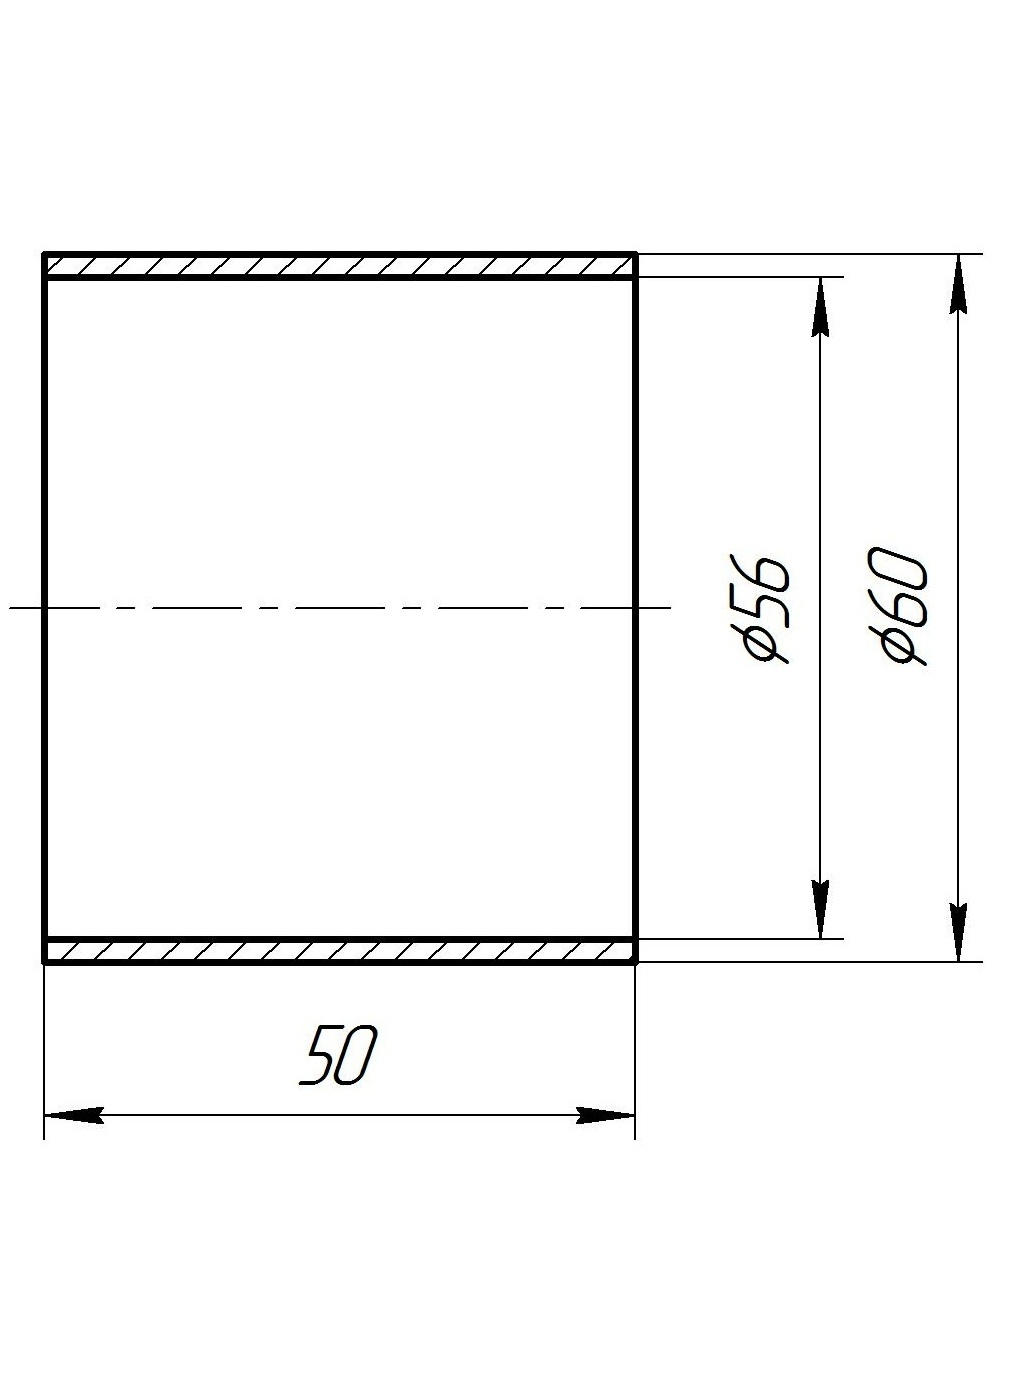
\includegraphics[width=.65\linewidth]{img/sketch}
			\captionof{figure}{Эскиз детали}
			\label{fig:sketch}
		\end{minipage}%
		\begin{minipage}{.5\textwidth}
			\centering
			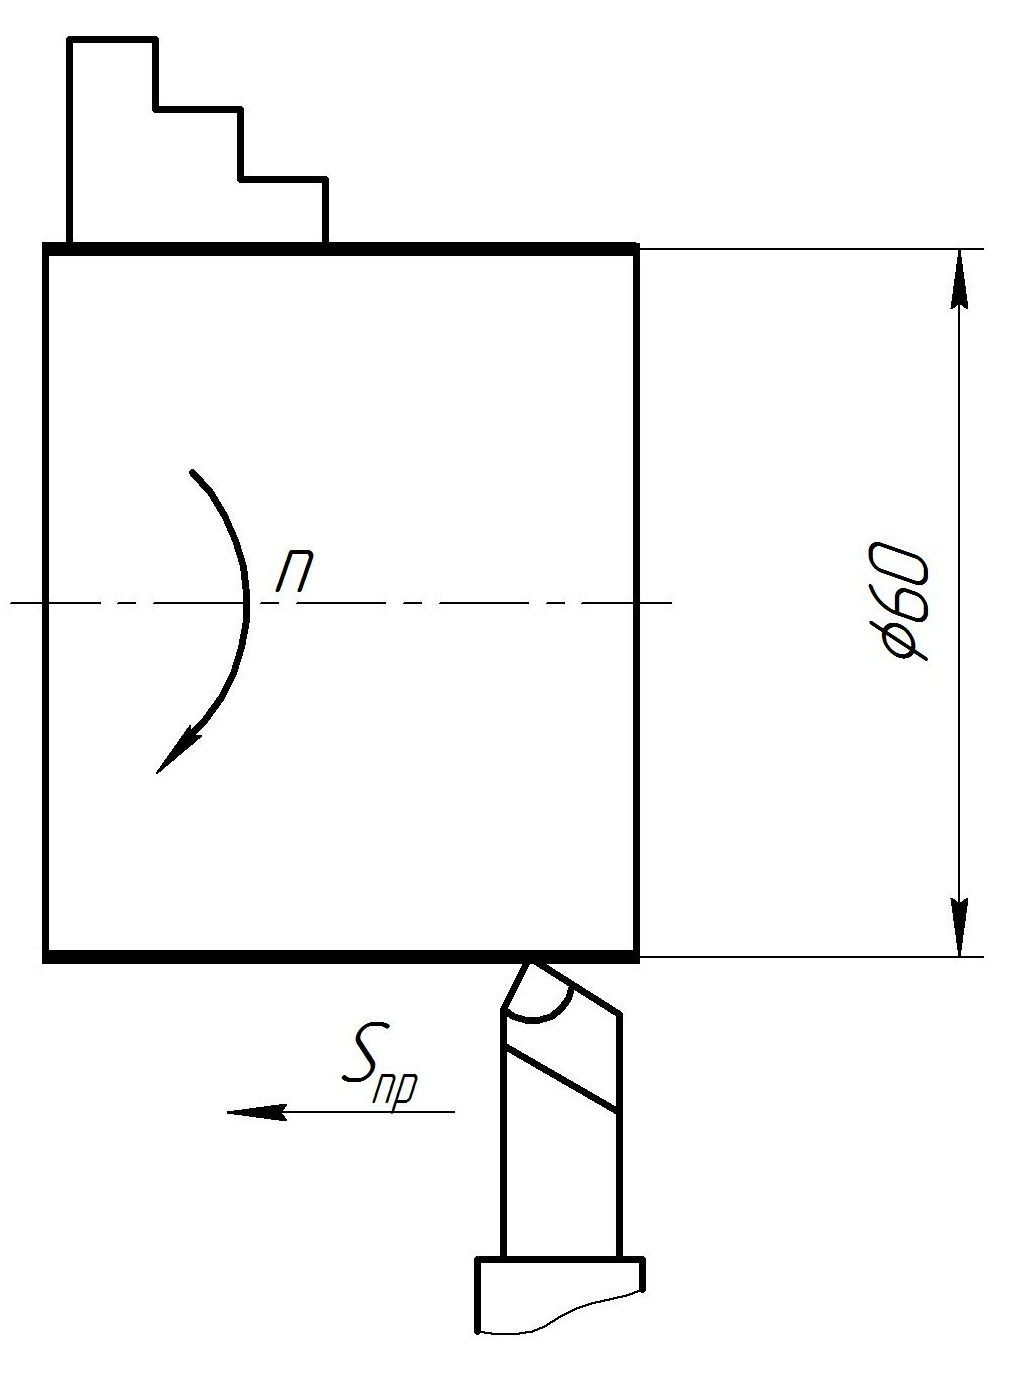
\includegraphics[width=.65\linewidth]{img/oper-sketch}
			\captionof{figure}{Операционный эскиз}
			\label{fig:oper-sketch}
		\end{minipage}
	\end{figure}
	
	\subsection{Выбор типа конечных элементов}
	Так как заданная деталь относится к типу тонкостенных, то наиболее подходящим элементом разбиения является оболочковый. Как рекомендует документация Abaqus для общего применения при достаточно больших напряжениях следует назначить элемент типа S4R. Название этого элемента расшифровывается как \textbf{S}hell, \textbf{4}-node, \textbf{R}educed integration, то есть оболочковый, 4-х узловой, с уменьшенным числом точек интегрирования .
	
	\begin{figure}[!h]
		\begin{center}
				\begin{overpic}[scale=1.3]{img/S4R}
					\put (60,-7) {1}
					\put (5,20) {2}
					\put (50,47) {3}
					\put (95,20) {4}		
				\end{overpic}
		\end{center}
		\caption{Оболочковый элемент S4R}
		\label{fig:S3R}
	\end{figure}
		
	Для нахождения матрицы жесткости элементов требуется вычислять интегралы вида
	$ \int_{-1}^{1} f(\xi) d\xi $ или для двухмерного случая $ \int_{-1}^{1}\int_{-1}^{1} f(\xi, \eta) d\xi d\eta $. Аналитически вычислить значения указанных выражений в общем случае не удается, поэтому применяют численные методы. Интеграл заменяется суммой:
	\begin{equation}\label{eq:FEAint}
		 \int_{-1}^{1} f(\xi) d\xi  \approx \sum_{i=1}^{n}a_if(\xi_i)
	\end{equation} 
	где $\xi_i$~--~точки интегрирования;\newline
	\phantom{где\space}$a_i$~--~весовые коэффициенты.
	
	Точки интегрирования выбираются исходя из конкретного метода интегрирования, но всегда при $ n\rightarrow \infty $ должно выполняться условие:
	\[ \sum_{i=1}^{n}a_if(\xi_i) \rightarrow \int_{-1}^{1} f(\xi) d\xi \]
	В МКЭ желательно применять такие методы выбора точек интегрирования и весовых коэффициентов, которые обеспечивали бы наибольшую точность при наименьшем числе точек интегрирования ввиду трудоемкости вычисления значения $ f(\xi_i) $. Поэтому применяется метод Гаусса, согласно которому точки $ \xi_i $ и коэффициенты $ a_i $ выбираются таким образом, чтобы формула (\ref{eq:FEAint}) представляла собой точное равенство для $ f(\xi)=1,\:\xi,\:\xi^2,\:...\:, \:\xi^p $. Так как число варьируемых величин в методе Гаусса равно $ 2n $, где $ n $~--~число точек интегрирования, то максимальный порядок интегрирования $ p\leq2n-1 $. 
		
	\begin{figure*}[h!]
		\centering
		\begin{subfigure}[t]{0.5\textwidth}
			\begin{overpic}[scale=.7]{img/FEAintpoints1}
				\put (90,48) {Узлы}
				\put (90,32) {Точки интегрирования}	
			\end{overpic}
			\caption{Полное интегрирование S4} \label{fig:FEAintpoints-a}
		\end{subfigure}%
		~ 
		\begin{subfigure}[t]{0.5\textwidth}
			\centering
			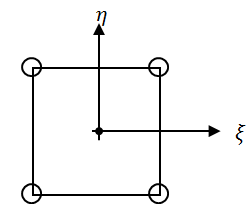
\includegraphics[scale=0.7]{img/FEAintpoints2}
			\caption{Сокращенное интегрирование S4R} \label{fig:FEAintpoints-b}
		\end{subfigure}
		\caption{Точки интегрирования} \label{fig:elements}
	\end{figure*}
	
	В случае плоского четырехузлового элемента подынтегральная функция $ f(\xi,\eta) $ является квадратичной по координатам $ \xi $ и $ \eta $, т.е. $ p=2 $ и $ n=2 $. Координаты две, поэтому говорят, что интегрирование осуществляется по $2\times 2 $ точкам. Такое интегрирования называется полным (\mbox{рисунок \ref{fig:FEAintpoints-a}}). Для уменьшения объема вычислений используется сокращенное число точек интегрирования. Для элемента S4R используется одна точка с координатами $ \xi=0, \eta=0 $ как показано на рисунке \ref{fig:FEAintpoints-b}.
	
	Кулачки моделируются пространственным элементом C3D8R~--~\textbf{C}ontinuum stress/displacement, \textbf{3D}~--~three-dimensional, \textbf{8}-node, \textbf{R}educed integration, то есть 8-ми узловой элемент для моделирования непрерывных полей напряжений/перемещений с уменьшенным числом точек интегрирования. 
	
	\subsection{Допущения}
	При построении модели воздействие резца на деталь учитывается в виде точечной трехкомпонентной силы, нагрев детали в рассмотрение не принимается. Считается, что сила резания в процессе обработки постоянна, глубина резания не изменяется, материал заготовки однородный. Кулачки моделируются в виде жестких ($E_\textup{кулачка} \gg E_\textup{детали} $) прямоугольных параллелепипедов, равномерно со всех сторон обхватывающих заготовку. 
	
	\subsection{Параметры модели}
	Для повышения эффективности работы разработчика моделей следует заранее составлять хорошо параметризованные модели. При достаточно большом числе параметров появляется возможность использовать одну модель для расчета нескольких деталей.  
	
	В таблице \ref{tab:model-params} приведены все изменяемые параметры для моделирования процесса обработки заданной детали, сгруппированные в трех категориях. Для детали параметрами полностью задается геометрические размеры и свойства материала. Аналогичные параметры выделены и для кулачков, но в эту категорию также добавлена величина радиального смещения и количество кулачков. Сила резания задается координатами точки приложения в цилиндрической системе координат  и тремя компонентами. 
	
	\newpage
	\begin{table}[h!]
		\centering
		\caption{Параметры модели}
		\label{tab:model-params}
		\begin{tabularx}{\textwidth}{|c|p{5.5cm}|M|}
			\hline
			Обозн. & Название & Схема \\
			\hline
			\multicolumn{3}{|Z|}{\textbf{Деталь}} \\ \hline
			L & Длина детали  & \multirow{5}{*}{\hfil \hspace{1cm} \parbox[c]{1em}{\centering\vspace{.1\baselineskip}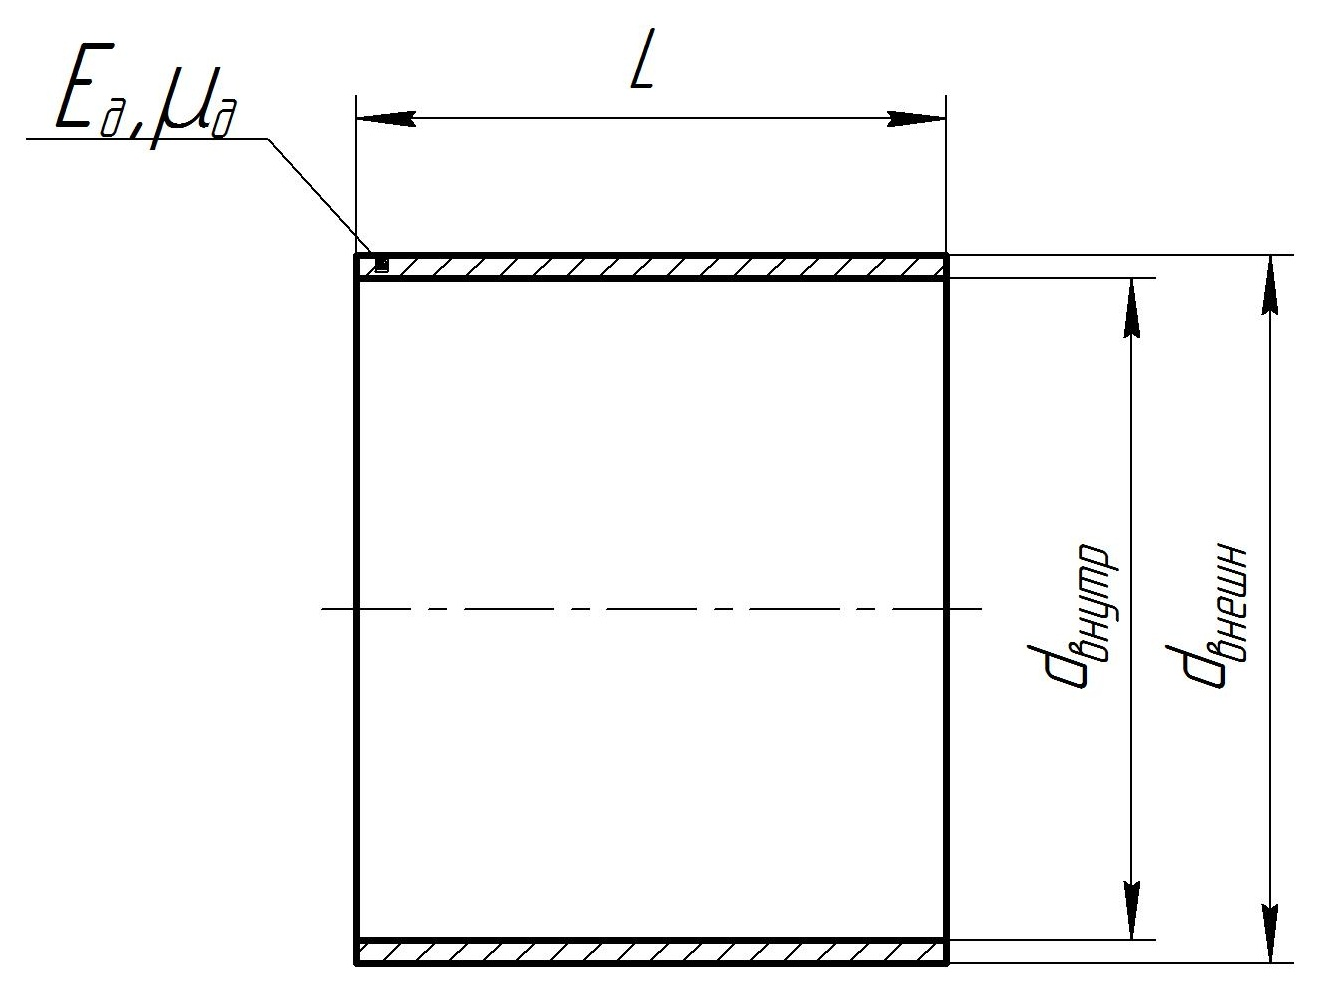
\includegraphics[scale=0.55]{img/param-part}}} \\ \cline{1-2}
			$ d_\textup{внутр} $ & Внутренний диаметр  &                   \\ \cline{1-2}
			$ d_\textup{внешн} $ & Внешний диаметр  &                   \\ \cline{1-2}
			$ E_\textup{д} $ & Модуль упругости \newline материала детали  &                   \\ \cline{1-2}
			$ \mu_\textup{д} $ & Коэффициент Пуассона \newline материала детали  &                   \\ \hline
			\multicolumn{3}{|Z|}{\textbf{Сила резания}} \\ \hline
			$ F_a $ & Осевая компонента \vspace{0.1\baselineskip} & \multirow{5}{*}{\hfil \parbox[c]{1em}{\vspace{.1\baselineskip}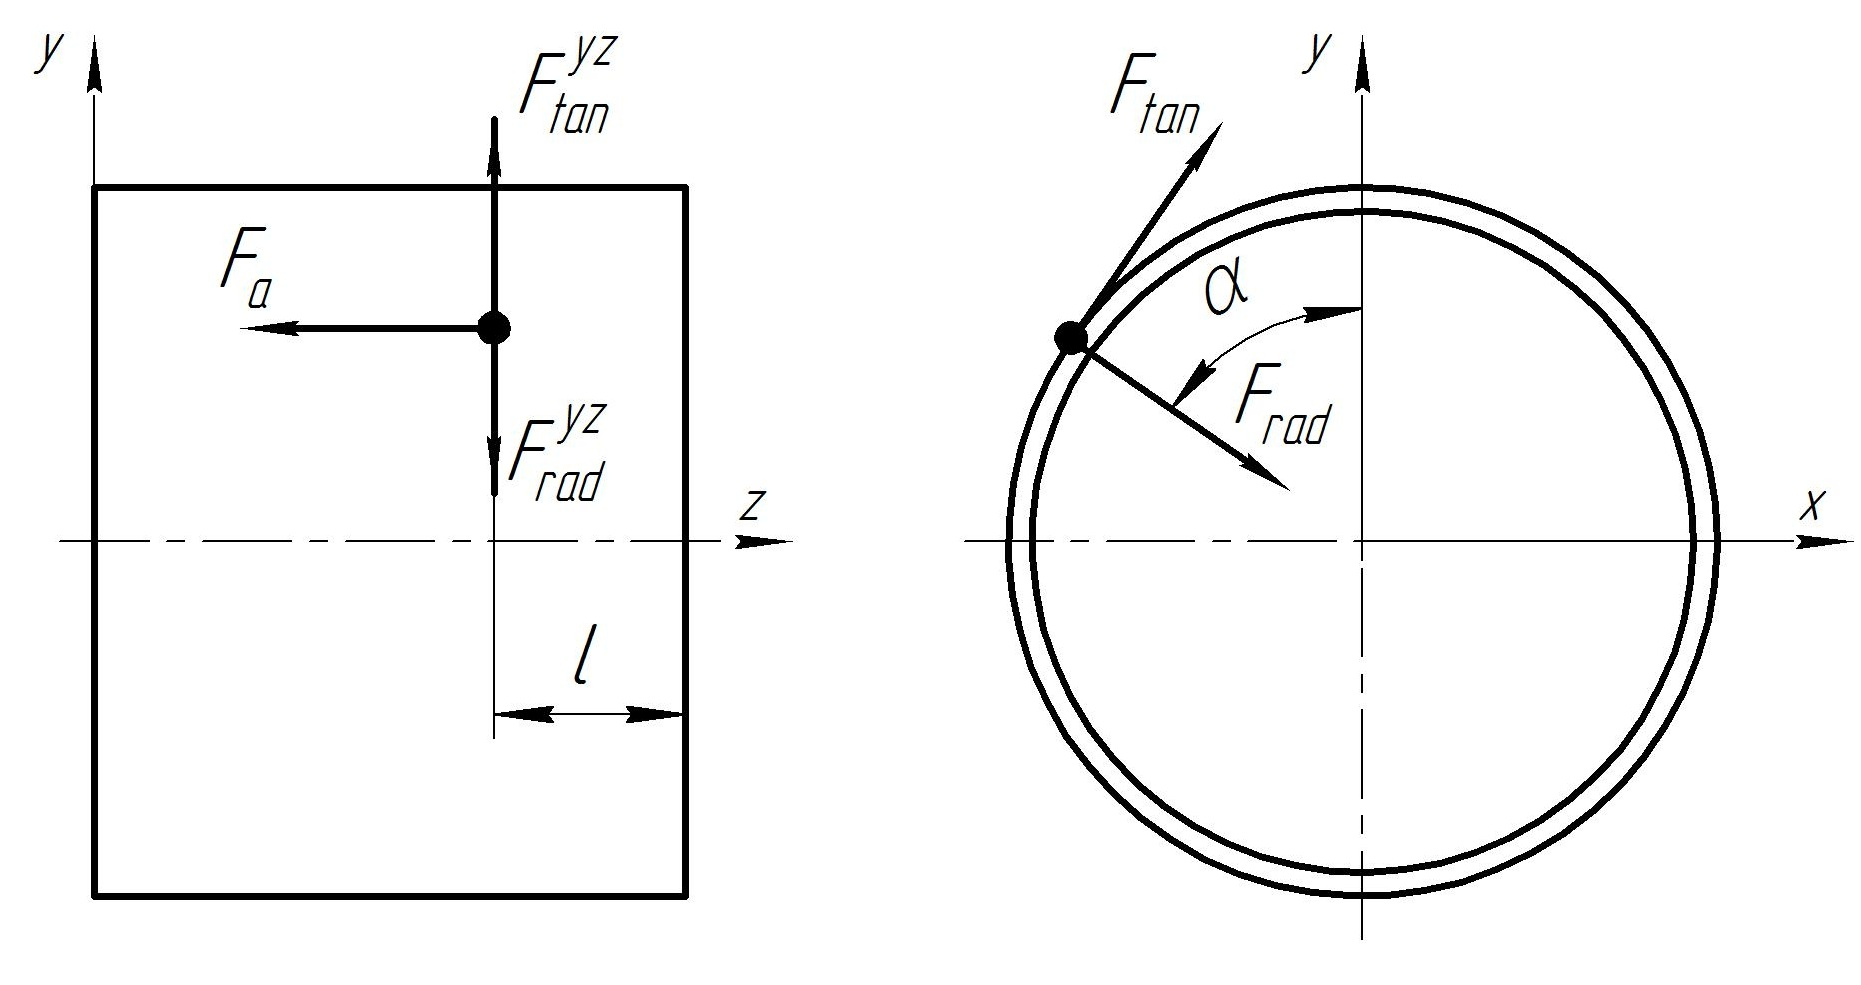
\includegraphics[scale=0.55]{img/param-force}}} \\ \cline{1-2}
			$ F_{tan} $ & Тангенциальная компонента  &                   \\ \cline{1-2}
			$ F_{rad} $ & Радиальная компонента &                   \\ \cline{1-2}
			$ l $ & Осевое положение \newline точки приложения &                   \\ \cline{1-2}
			$ \alpha $ & Угловое положение \newline точки приложения  &                   \\ \hline
			\multicolumn{3}{|Z|}{\textbf{Кулачки}} \\ \hline
			$ \Delta $ & Радиальное смещение  & \multirow{5}{*}{\hfil \hspace{1cm} \parbox[c]{1em}{\vspace{.1\baselineskip}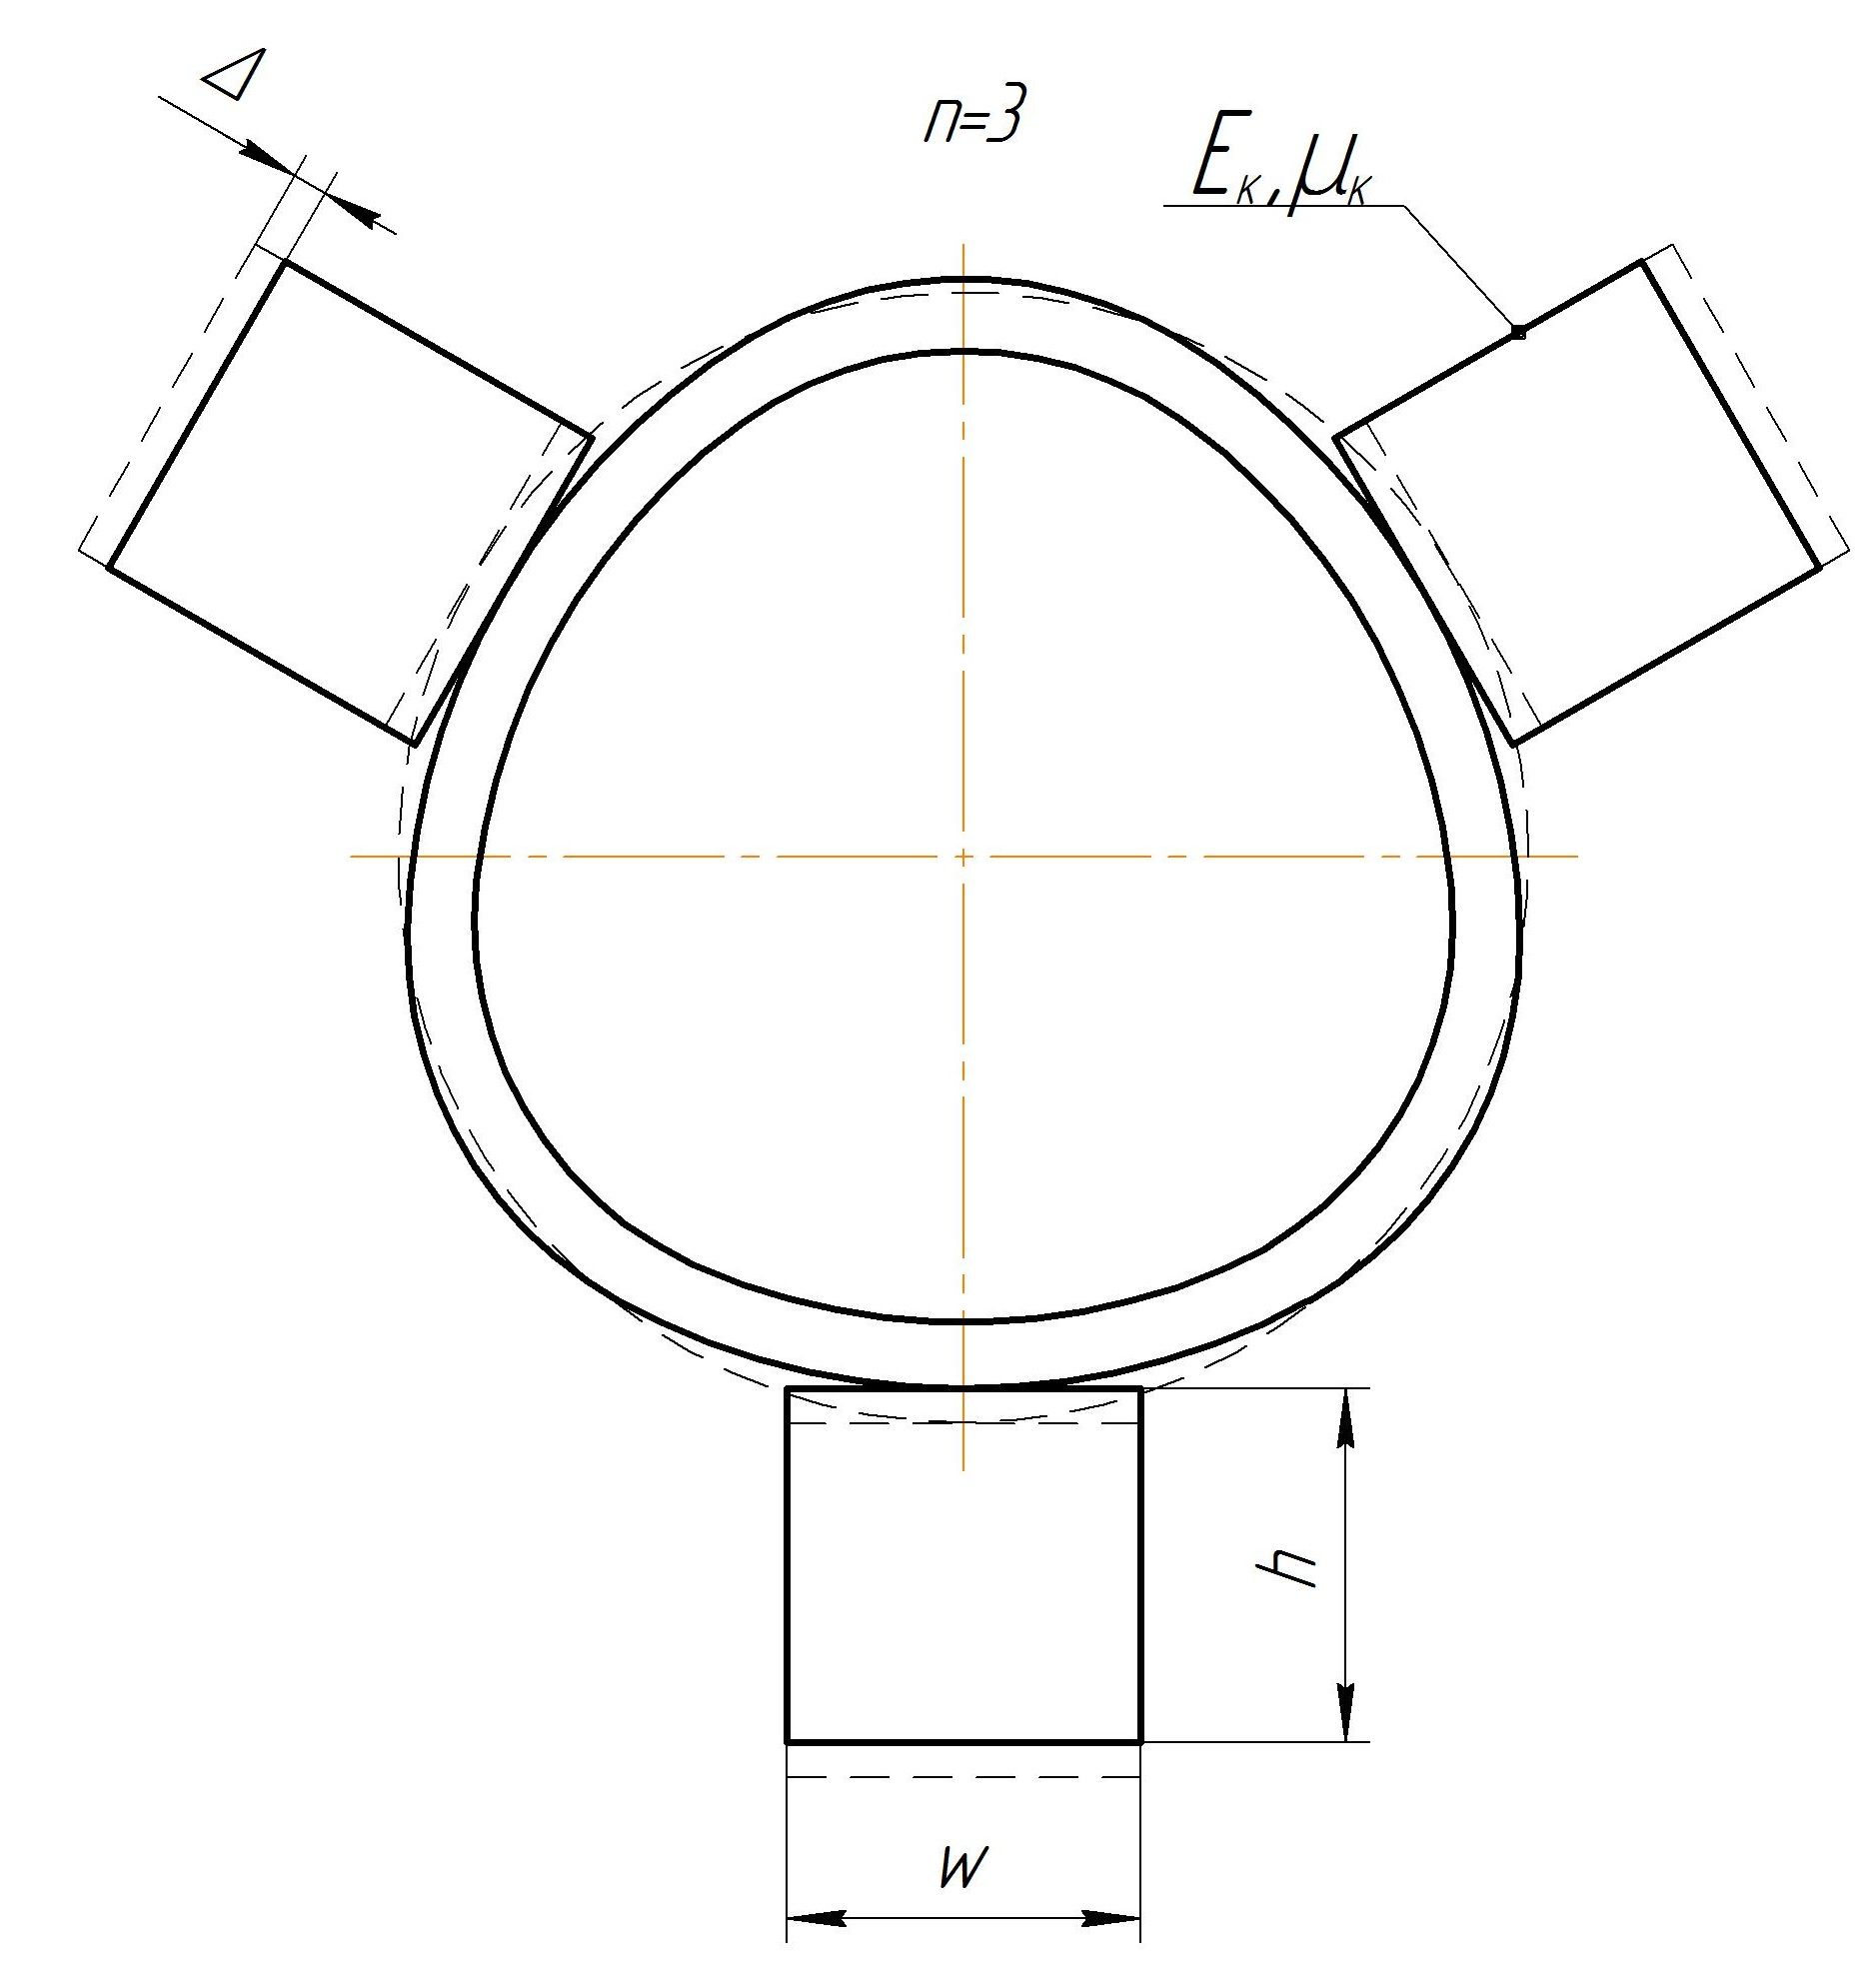
\includegraphics[scale=0.40]{img/param-jaw}}} \\ \cline{1-2}
			$ n $ & Количество кулачков  &                   \\ \cline{1-2}
			 w  & Ширина кулачка &                   \\ \cline{1-2}
			 h  & Высота кулачка &                   \\ \cline{1-2}
			$ t $ & Толщина кулачка  &                   \\ \cline{1-2}
			$ E_\textup{к} $ & Модуль упругости \newline материала кулачков  &                   \\ \cline{1-2}
			$ \mu_\textup{к} $ & Коэффициент Пуассона \newline материала кулачков  &                   \\ \hline
		\end{tabularx}
	\end{table}
	
	\subsection{Модель в Abaqus}
	На рисунке \ref{fig:abaqus-model} показана построенная модель и её разбиение на конечные элементы. Построение модели полностью автоматизировано благодаря применению встроенного в Abaqus языка сценариев.

	\begin{figure*}[h!]
		\centering
		\begin{subfigure}[t]{0.5\textwidth}
			\centering
			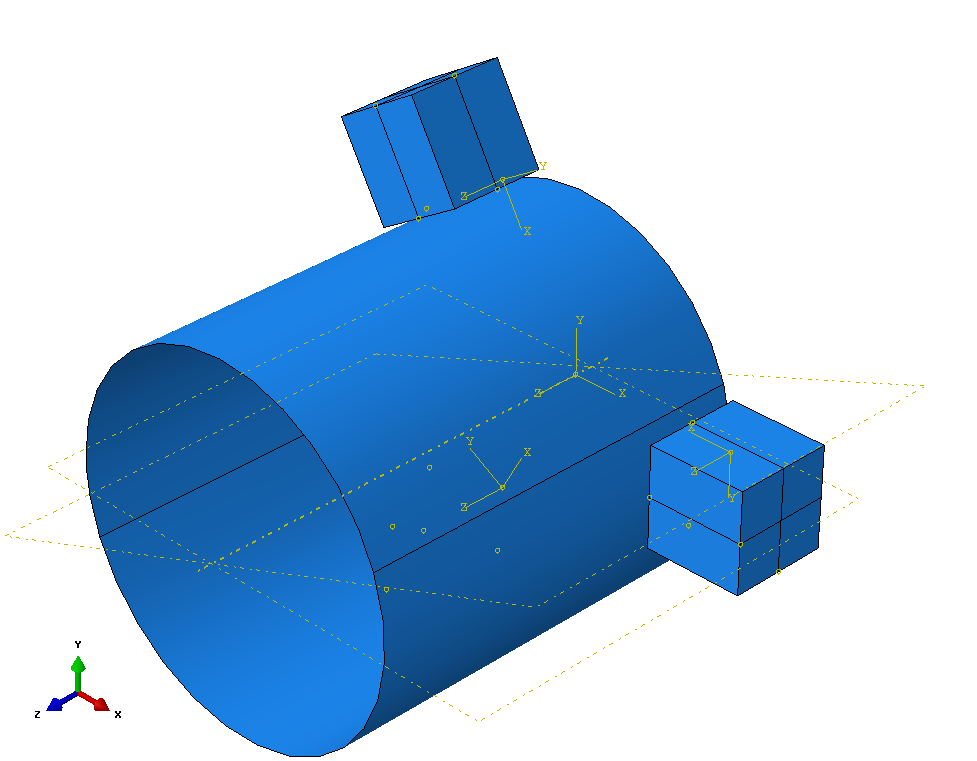
\includegraphics[scale=0.28]{img/model} 
			\caption{Модель} \label{fig:abaqus-model-a}
		\end{subfigure}%
		~ 
		\begin{subfigure}[t]{0.5\textwidth}
			\centering
			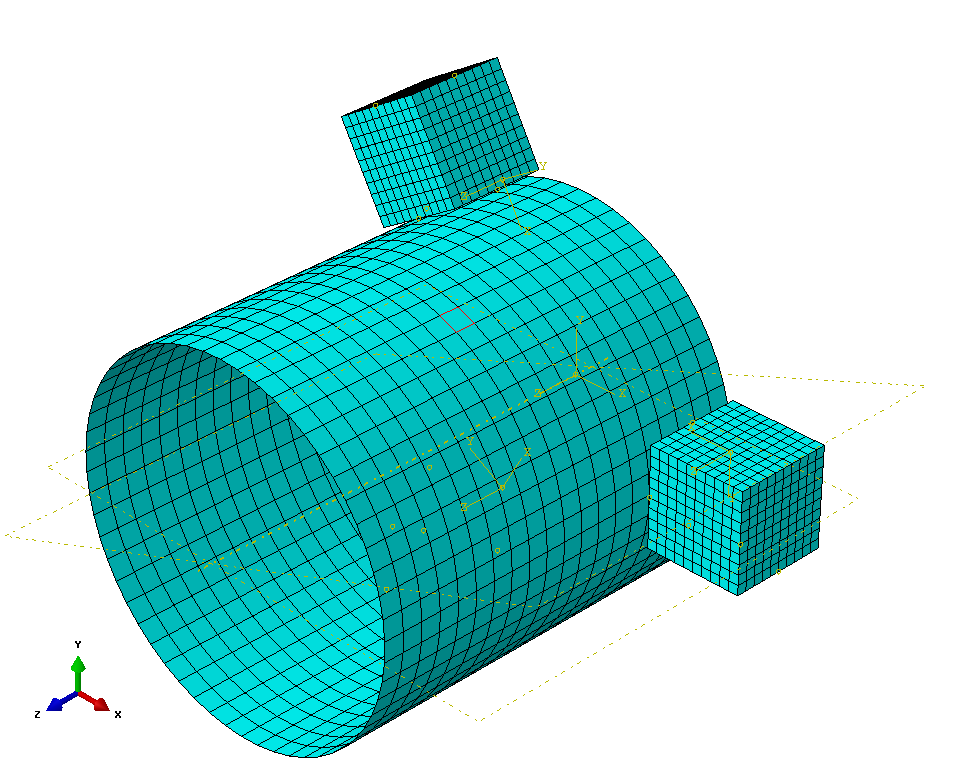
\includegraphics[scale=0.28]{img/modelMesh} 
			\caption{Сетка} \label{fig:abaqus-model-b}
		\end{subfigure}
		\caption{Модель в Abaqus} \label{fig:abaqus-model}
	\end{figure*}

	Для приложения силы резания в точке, соответствующей заданным координатам, применяется вспомогательное сечение 	плоскостью, расположенной под углом $ \alpha $ к центральной плоскости кулачка. 
	 
	\begin{figure}[!h]
		\begin{center}
			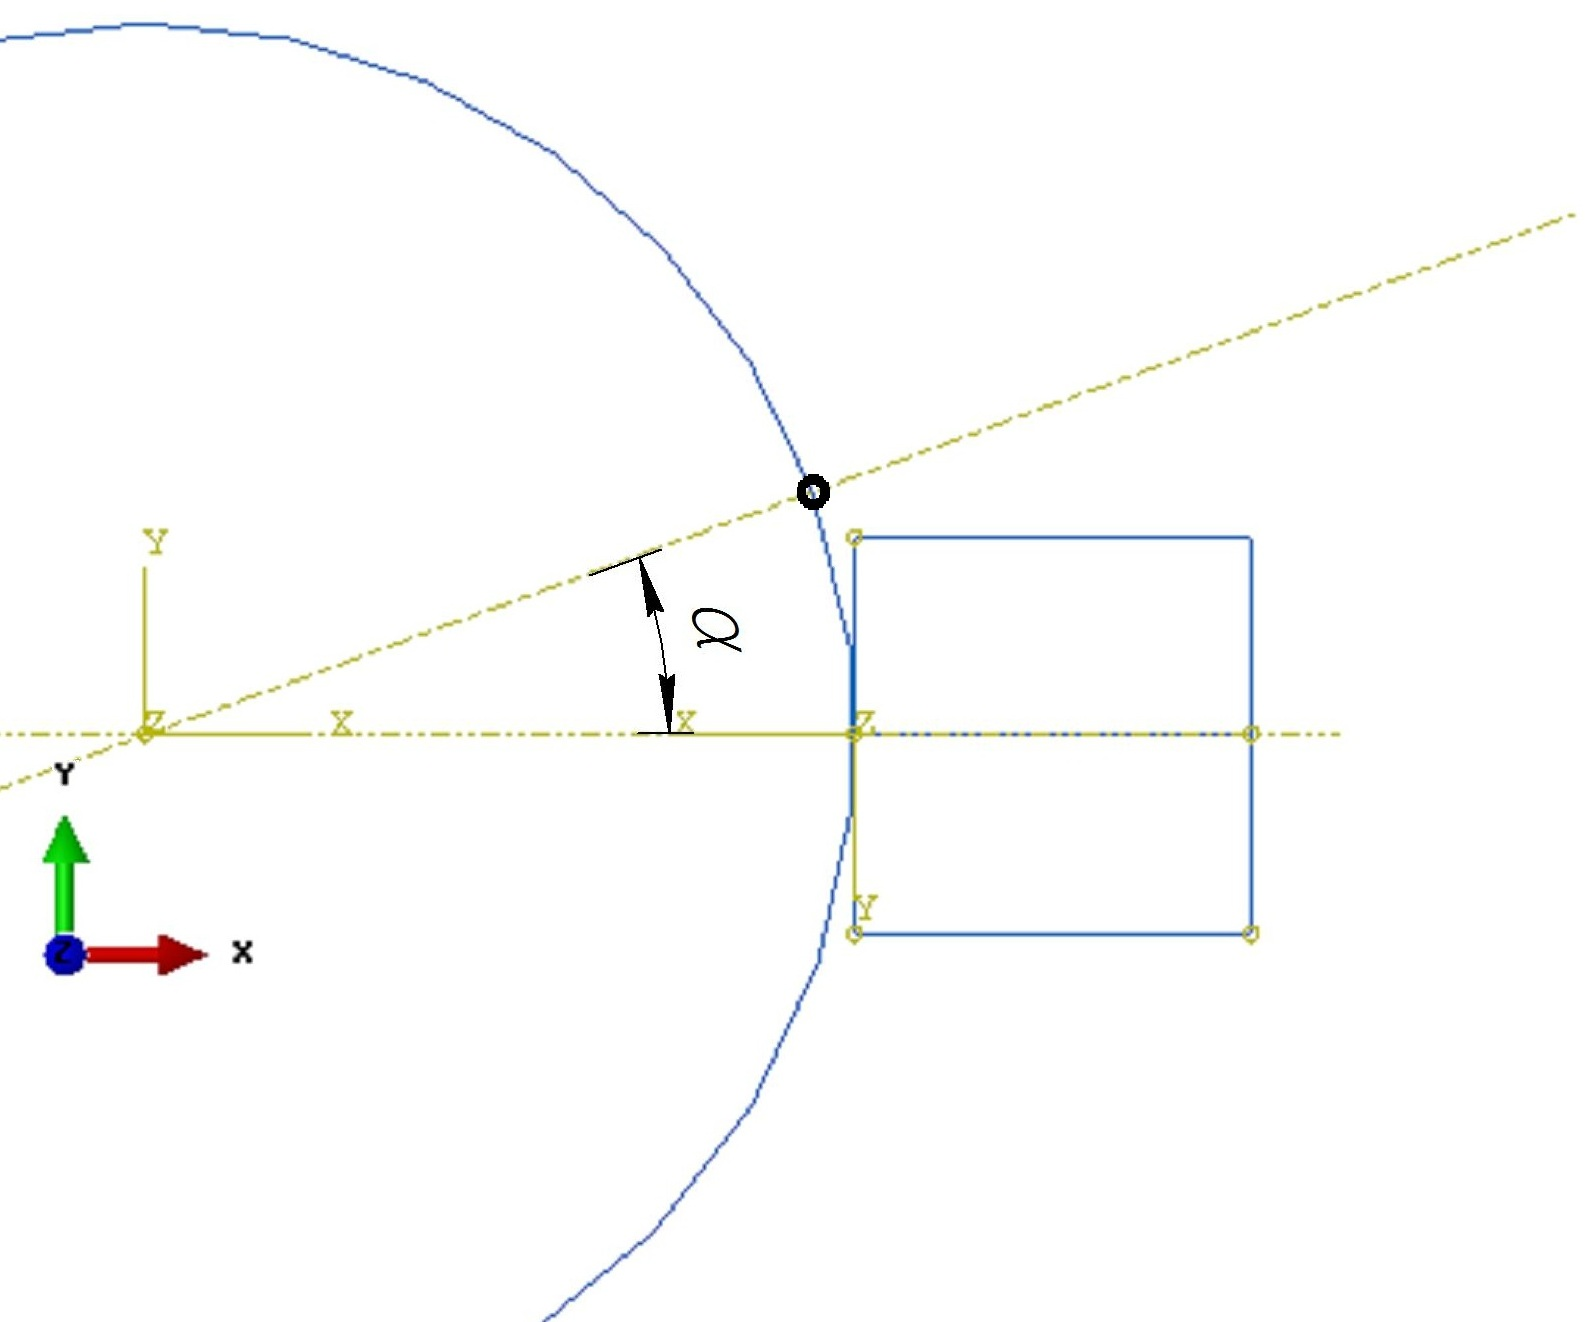
\includegraphics[scale=0.5]{img/modelPlane} 
		\end{center}
		\caption{Вспомогательное сечение}
		\label{fig:model-plane}
	\end{figure} 
	 
	На рисунке  \ref{fig:abaqus-results} показаны поля напряжения и деформаций. На диаграмме напряжений отчетливо видна точка приложения силы резания. Как было сказано выше, жесткость кулачков намного больше жесткости самой детали, поэтому изменения напряжений и деформаций на них не могут быть отображены в данном масштабе.  
	
	\begin{figure*}[h!]
		\centering
		\begin{subfigure}[t]{0.5\textwidth}
			\centering
			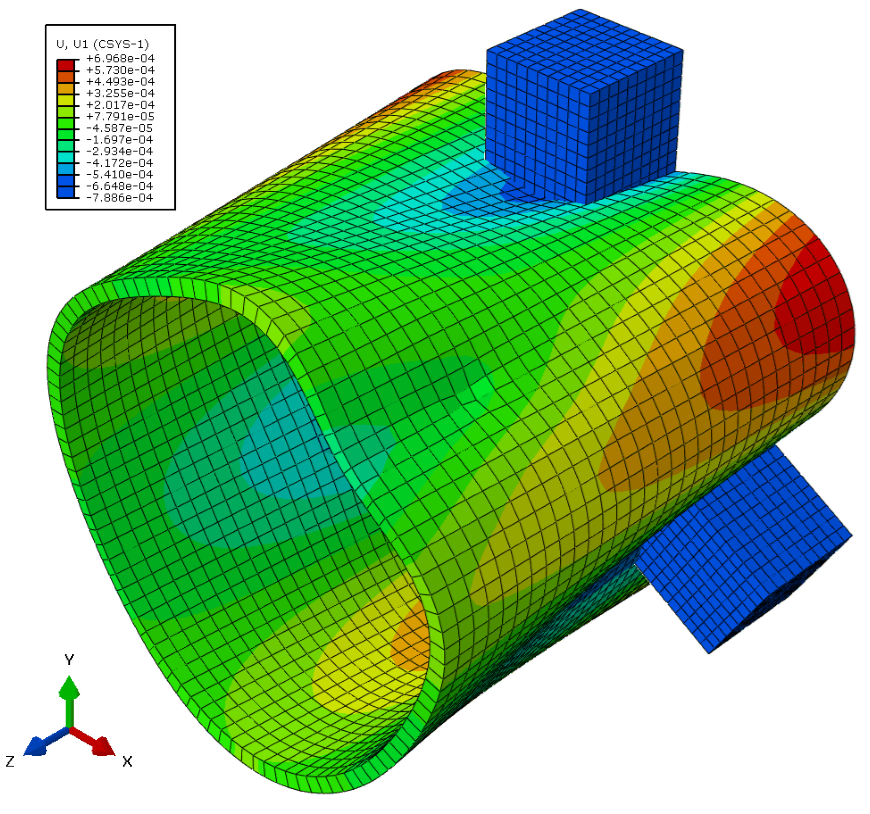
\includegraphics[scale=0.27]{img/diagram-displ}
			\caption{Узловые перемещения} \label{fig:digram-displ}
		\end{subfigure}%
		~ 
		\begin{subfigure}[t]{0.5\textwidth}
			\centering
			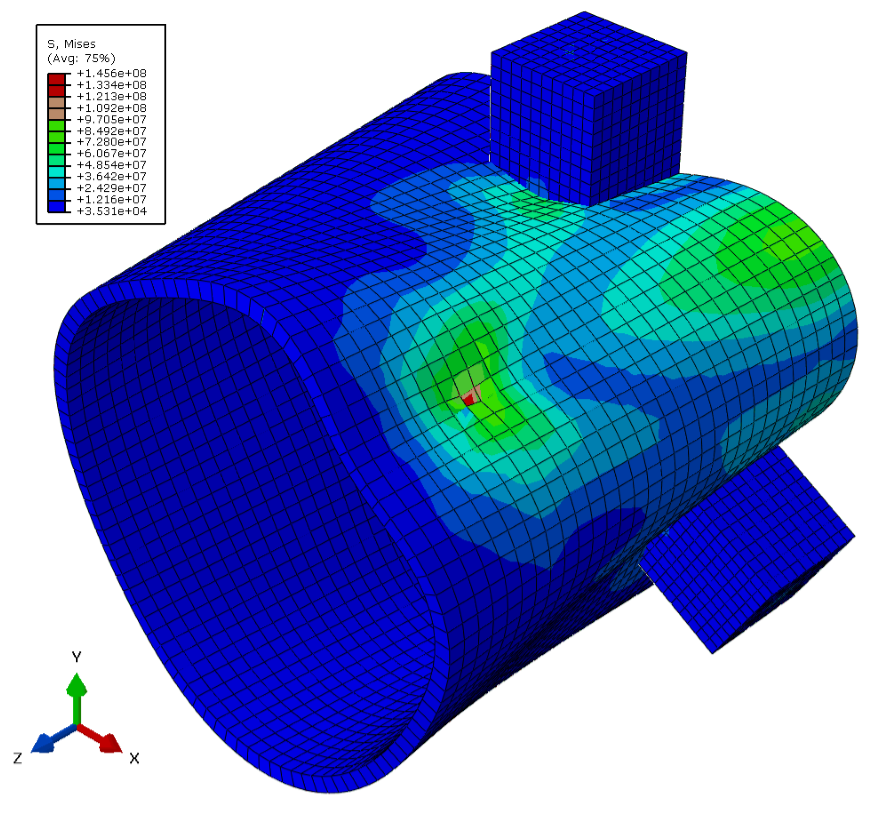
\includegraphics[scale=0.27]{img/diagram-stress} 
			\caption{Напряжения} \label{fig:digram-stress}
		\end{subfigure}
		\caption{Результаты расчета} \label{fig:abaqus-results}
	\end{figure*} 

	\section{Разработка калькулятора резания}
	Калькулятор режимов резания разрабатывается в виде отдельной подсистемы, физически реализованной как  модуль платформы NetBeans. Он служит для определения начального приближения значений сил резания и предполагает использование таблично-аналитической методики, описанной в \cite{book:Kosilova}. Структура исходных данных, определенная на этапе эскизного проектирования не нуждается в уточнении.
	
	Рассматриваемая таблично-аналитическая методика использует большое количество эмпирических коэффициентов, которые могут на самом деле отличаться от приведенных справочных значений. Поэтому было принято решение организовать вычисление режимов резания по гибкой технологии, в основе которой лежит использование баз знаний. 
	
	\subsection{Библиотека Drools}	
	Для Java существует бесплатная библиотека с открытым исходным кодом Drools. Эта библиотека позволяет осуществлять логический вывод, основанный на использовании продукционных правил. На рисунке \ref{fig:drools-alg} показан алгоритм работы машины вывода Dools согласно официальной документации \cite{web:DroolsOfficial}. Рабочая память сопоставляется с база правил для определения конфликтного множества, то есть набора правил, которые могут быть выполнены в данный момент. При помощи заданной стратегии разрешения конфликтов из конфликтного множества определяется единственное правило, которое затем исполняется. Процесс повторяется пока существует хотя бы одно правило для выполнения или пока не произойдет выход при выполнении одного из правил.
				
	
	\begin{figure}[!h]
		\begin{center}
			\begin{overpic}[width=1\textwidth]{img/drools-alg}
				\put (0.3,28) {\small Выполнить}	
				\put (2,26) {\small правило}
				\put (28.3,28) {\small Правило}	
				\put (28.5,26) {\small найдено}	
				\put (60,3) {\small Выход}	
				\put (59,15) {\small Правило}	
				\put (58,13) {\small не найдено}	
				\put (59.3,29.5) {\small Выбрать}	
				\put (57,27.5) {\small правило для }			
				\put (57.3,25.5) {\small выполнения}	
				\put (10,4.5) {\small Выйти, если указано}
				\put (10,2.5) {\small правилом}
				\put (17,46) {\small Рабочая}	
				\put (17,44) {\small память}	
				\put (17,65) {\small База}	
				\put (17,63) {\small правил}	
				\put (50,41) {\small Конфликтное множество}	
				\put (86,29) {\small Стратегия}	
				\put (85,27) {\small разрешения}	
				\put (85,25) {\small конфликтов}					
				\put (52,56) {\small Определить правила,}					
				\put (52,54) {\small которые могут быть}					
				\put (52,52) {\small выполнены}					
			\end{overpic}
		\end{center}
		\caption{Алгоритм работы Drools}
		\label{fig:drools-alg}
	\end{figure}

	\subsection{Запись продукционных правил}			
	Продукционные правила могут быть записаны в двух видах. Первый способ заключается в последовательном перечислении в текстовом файле всех правил, составленных на специализированном языке DRL - Drools Rule Language. Этот язык позволяет записывать правила в следующем виде:
	\vspace{0.5cm}
	\lstset{emph={attributes}, emphstyle=\itshape}
	\begin{lstlisting}
	rule "name"
			attributes
		when
			LHS
		then
			RHS
	end
	\end{lstlisting}
	
	В приведенном фрагменте используются обозначения: {\tt name} - имя правила; {\tt LHS} - левая часть правила, то есть предусловие, которое должно быть соблюдено, чтобы правило сработало; {\tt RHS} - правая часть правила, содержащая код, который выполняется в случае срабатывания правила; {\tt \textit{attributes}} - специальные атрибуты, модифицирующие работу правил. Например, формула $ N = P_zV/1020\cdot60 $ для вычисления мощности резания, в виде продукционного правила представляется следующим образом:  
	\vspace{0.5cm}
	\begin{lstlisting} 
	rule "Calculate N" 
		salience -140
		lock-on-active true
		when
			step : TurningStepBean ()
		then
			modify(step){setN(step.P*step.v/(1020*60))}
	end
	\end{lstlisting}
	
	Приведенное правило имеет низкий приоритет (задается после ключевого слова {\tt salience}), поэтому оно будет проверяться только после того как будут выбраны все необходимые эмпирические коэффициенты. Приоритет правил позволяет упорядочить их таким образом, чтобы не возникало недостатка данных. Это можно пояснить на следующем примере: формула вычисления мощности резания  $ N = P_zV/1020\cdot60 $ требует известных значений силы $ P_z $ и скорости резания $ V $, поэтому соответствующее продукционное правило имеет приоритет ниже, чем приоритет формул  $ V=\dfrac{C^v}{T^m\,t^x\,s^y}K_{MV}K_{MP}K_{\textup{ИV}} $ и $ P_z=10\,C_p \, t^x s^y V^n K_{MP} $.
		
		\begin{figure}[!h]
			\begin{center}
				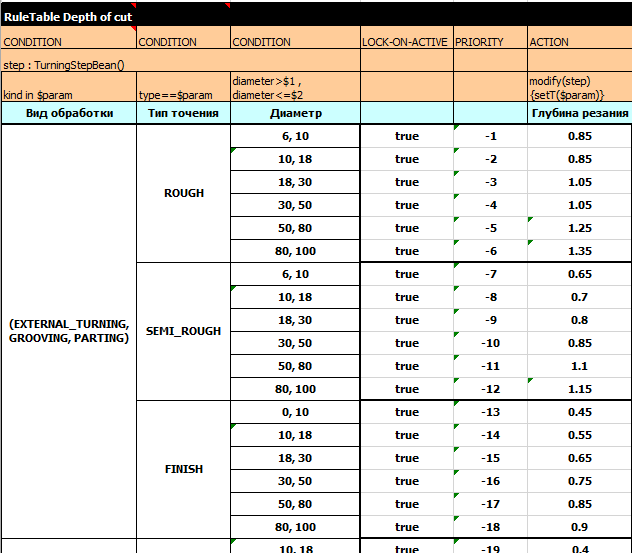
\includegraphics[width=\textwidth]{img/rules-table-excel} 
			\end{center}
			\caption{Продукционные правила в виде Excel таблиц (фрагмент)}
			\label{fig:rules-table-excel}
		\end{figure}  
	
	Расчет режимов резания по формулам основывается на значениях предварительно выбранных эмпирических коэффициентов. Для назначения коэффициентов используется второй вид записи знаний в Drools - в виде Excel таблиц. Фрагмент таблицы для определения глубины резания показан на рисунке \ref{fig:rules-table-excel}. Столбцы таблицы решений Drools могут быть отмечены ключевыми словами, в данном случае используются следующие: 
	\begin{itemize}
		\setlength\itemsep{0em}
		\item[]	\texttt{CONDITION}~--~условие, то есть такой столбец соответствует левой части продукционного правила
		\item[]	\texttt{LOCK-ON-ACTIVE}~--~запрещает выполнение других правил во время выполнения данного правила
		\item[]	\texttt{PRIORITY}~--~приоритет, определяет порядок проверки правил
		\item[]	\texttt{ACTION}~--~действие, соответствует правой части правила
	\end{itemize}

	 В приведенной таблице запись \texttt{step : TurningStepBean()} означает, что для выполнения постусловия необходимо, чтобы в рабочей памяти находился объект класса \texttt{TurningStepBean}. Если такой объект будет найден, то он будет доступен по ссылке \texttt{step}. Ячейки следующей строки проверяют свойства найденного объекта для столбцов условия или определяют действие над объектом в случае столбца действия. Таким образом, запись \texttt{kind in \$param} обозначает, что найденный объект должен удовлетворять определенному множеству значений по свойству \texttt{kind}. Соответствующее множество допустимых значений указывается в круглых скобках в ячейках ниже. Второй слева столбец предназначен для проверки типа точения, его условие записывается как \texttt{type==\$param}. Третий столбец описывает ограничения на диаметр заготовки. Например, для первой строки диаметр заготовки должен лежать в диапазоне от 6 до 10 мм. Столбцы \texttt{LOCK-ON-ACTIVE} и \texttt{PRIORITY} управляют выполнением правил. Последний столбец описывает действие над фактами рабочей области. В данном случае для объекта \texttt{step} устанавливается глубина резания при помощи инструкции \texttt{modify(step)\{setT(\$param)\}}. 
	 
	 Фактически все строки Excel таблицы на рисунке \ref{fig:rules-table-excel} во время выполнения компилируются в отдельные правила на языке DRL. Первая строка указанной таблицы компилируется следующим образом:
	\vspace{0.5cm}
	\begin{lstlisting} 
	rule "Depth of cut_10"
		salience -1
		lock-on-active true
		when
			step : TurningStepBean(kind in (EXTERNAL_TURNING, 
				   GROOVING, PARTING), type==ROUGH, 
				   diameter>6 , diameter<=10)
		then
			modify(step) {setT(0.85)}
	end
	\end{lstlisting}
	
	\subsection{Алгоритм вычисления}		
	Хотя в программной реализации калькулятора режимов резания и применяются современные технологии организации вычислений, тем не менее сам алгоритм соответствует таблично-аналитической методике, основанной на вычислении параметров режимов по формулам с эмпирическим коэффициентам. Исходные данные для алгоритма определены на этапе эскизного проектирования.
	
	Алгоритм вычисления описывается последовательностью следующих действий:
	\begin{enumerate}
		\item Выбор значения глубины резания $ t $ из таблицы \ref{tab:glubina}
		\item Выбор значения подачи $ s $ из таблицы \ref{tab:podacha}
		\item Выбор поправочных коэффициентов $ C_\textup{v},\,T,\,m,\,y,\,K_\textup{MV},\,K_\textup{ПV},\,K_\textup{ИV} $ из таблиц \ref{tab:KMV}, \ref{tab:KPV}, \ref{tab:KIV}, \ref{tab:emp1}
		\item Вычисление скорости резания по формуле $ v=\dfrac{C^v}{T^m\,t^x\,s^y}K_{MV}K_{\textup{ПV}}K_{\textup{ИV}} $
		\item Выбор поправочных и эмпирических коэффициентов $ C_\textup{p},\,q,\,n,\,x,\,y $ из таблицы  \ref{tab:emp2}
		\item Вычисление частоты вращения по формуле $ n=\dfrac{1000v}{\pi D} $
		\item Вычисление силы резания по формуле $ P_z=10\cdot C_p\,t^x\,s^y\,v^n\,K_{MP} $
		\item Вычисление момента резания по формуле $ N=\dfrac{P_z\cdot v}{1020 \cdot 60}$
	\end{enumerate}
	
	Таблицы \ref{tab:glubina} -- \ref{tab:emp2} приведены в приложении \ref{app:tables}.

	\subsection{Графический интерфейс}
	Пользователь взаимодействует с модулем калькулятора режимов резания при помощи пользовательского интерфейса, который представлен в виде двух окон, изображенных на рисунке \ref{fig:calc-screen}.
		
	\begin{figure*}[h!]
		\centering
		\begin{subfigure}[t]{0.5\textwidth}
			\centering
			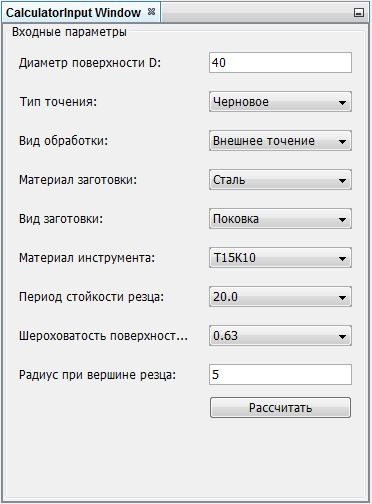
\includegraphics[width=1\textwidth]{img/calc-input-screen}
			\caption{Окно ввода} \label{fig:calc-input-screen}
		\end{subfigure}%
		~ 
		\begin{subfigure}[t]{0.5\textwidth}
			\centering
			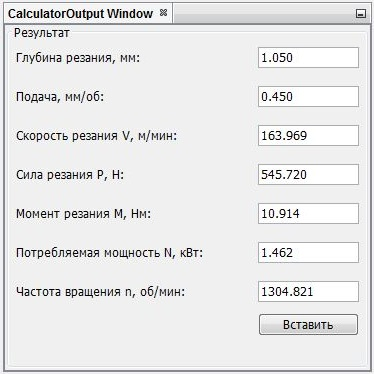
\includegraphics[width=1\textwidth]{img/calc-output-screen} 
			\caption{Окно результатов} \label{fig:calc-output-screen}
		\end{subfigure}
		\caption{Графический интерфейс калькулятора режимов резания} \label{fig:calc-screen}
	\end{figure*}
	
	Первое окно (рисунок \ref{fig:calc-input-screen}) служит для ввода исходных данных. Оно содержит два текстовых поля и несколько выпадающих списков для выбора возможных значений. Исходные данные для калькулятора режимов резания были подробно описаны на этапе эскизного проектирования, все варианты значений приведены в таблице \ref{tab:calc}.  
		
	Результат вычислений будет отображен в окне вывода информации (рисунок \ref{fig:calc-output-screen}) после нажатия на кнопку ``Рассчитать''. Кнопка ``Вставить'' служит для применения рассчитанных значений к модели и копирует значение силы резания в соответствующий параметр редактора моделей. 	

	\section{Модуль визуального отображения}	
	Модуль визуального отображения позволяет контролировать значения параметры при помощи интерактивной трехмерной модели заготовки. Для работы с пространственной геометрией и вывода её на экран используется библиотека JavaFX, входящая в состав JDK. 
	
	После загрузки базы данных или Excel таблиц в систему поддержки, происходит распаковка трехмерной модели в отдельный obj файл, располагающийся в текущей рабочей директории. Устройство формата obj достаточно простое для реализации преобразования файла в объекты JavaFX. Структура файла показана ниже. Из примера видно, что obj файл сохраняется в текстовом формате и содержит перечисление всех вершин модели, текстурных координат (в разрабатываемой системе не используются) а также нормалей и определений поверхностей. 
	
	\begin{lstlisting}[style=nonumbers]
	  |\# Список вершин, с координатами (x,y,z)|
	  v 0.123 0.234 0.345
	  v ...
	  ...
	  |\# Текстурные координаты (u,v)|
	  vt 0.500 -1.352
	  vt ...
	  ...
	  |\# Нормали (x,y,z), могут быть не нормированными.|
	  vn 0.707 0.000 0.707
	  vn ...
	  ...
	  |\# Определения поверхности(сторон) f v1 v2 v2|
	  f 1 2 3
	  f ...
	  ...
	\end{lstlisting} 

	Библиотека JavaFX позволяет отображать примитивы, такие как параллелепипед, цилиндр и более сложные полигональные модели при помощи класса \texttt{MeshView}. В рассматриваемом случае файл obj преобразуется в экземпляр \texttt{MeshView}, а вспомогательные тела (такие как оси координат) накладываются дополнительно при помощи примитивов. Окно модуля визуального отображения показано на рисунке \ref{fig:viewport-screen}.
	
	\begin{figure}[!h]
		\begin{center}
			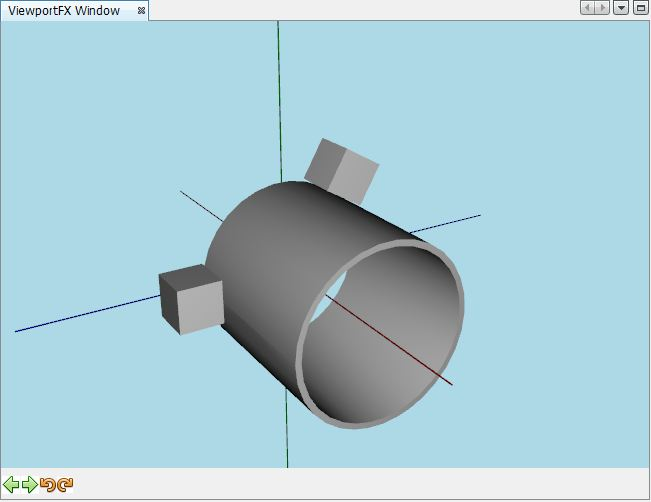
\includegraphics[scale=0.76]{img/viewport-screen} 
		\end{center}
		\caption{Модуль визуального отображения}
		\label{fig:viewport-screen}
	\end{figure}	 

	\section{Запуск Abaqus}	 
	Необходимо организовать выполнение сценариев Python скриптов в Abaqus. Данная задача может быть решена при помощи интерфейса командной строки. Вызов любой внешней команды возможен из языка Java при помощи класса \texttt{ProcessBuilder}. Этот класс позволяет создать новый процесс операционной системы с заданными аргументами. Для вызова заданного сценария потребуется указать только файл с расширением .py, содержащий код на языке Python. Если модель параметризована, то потребуется также передача всех фактических значений параметров.
		
	\begin{figure}[!h]
		\begin{center}
			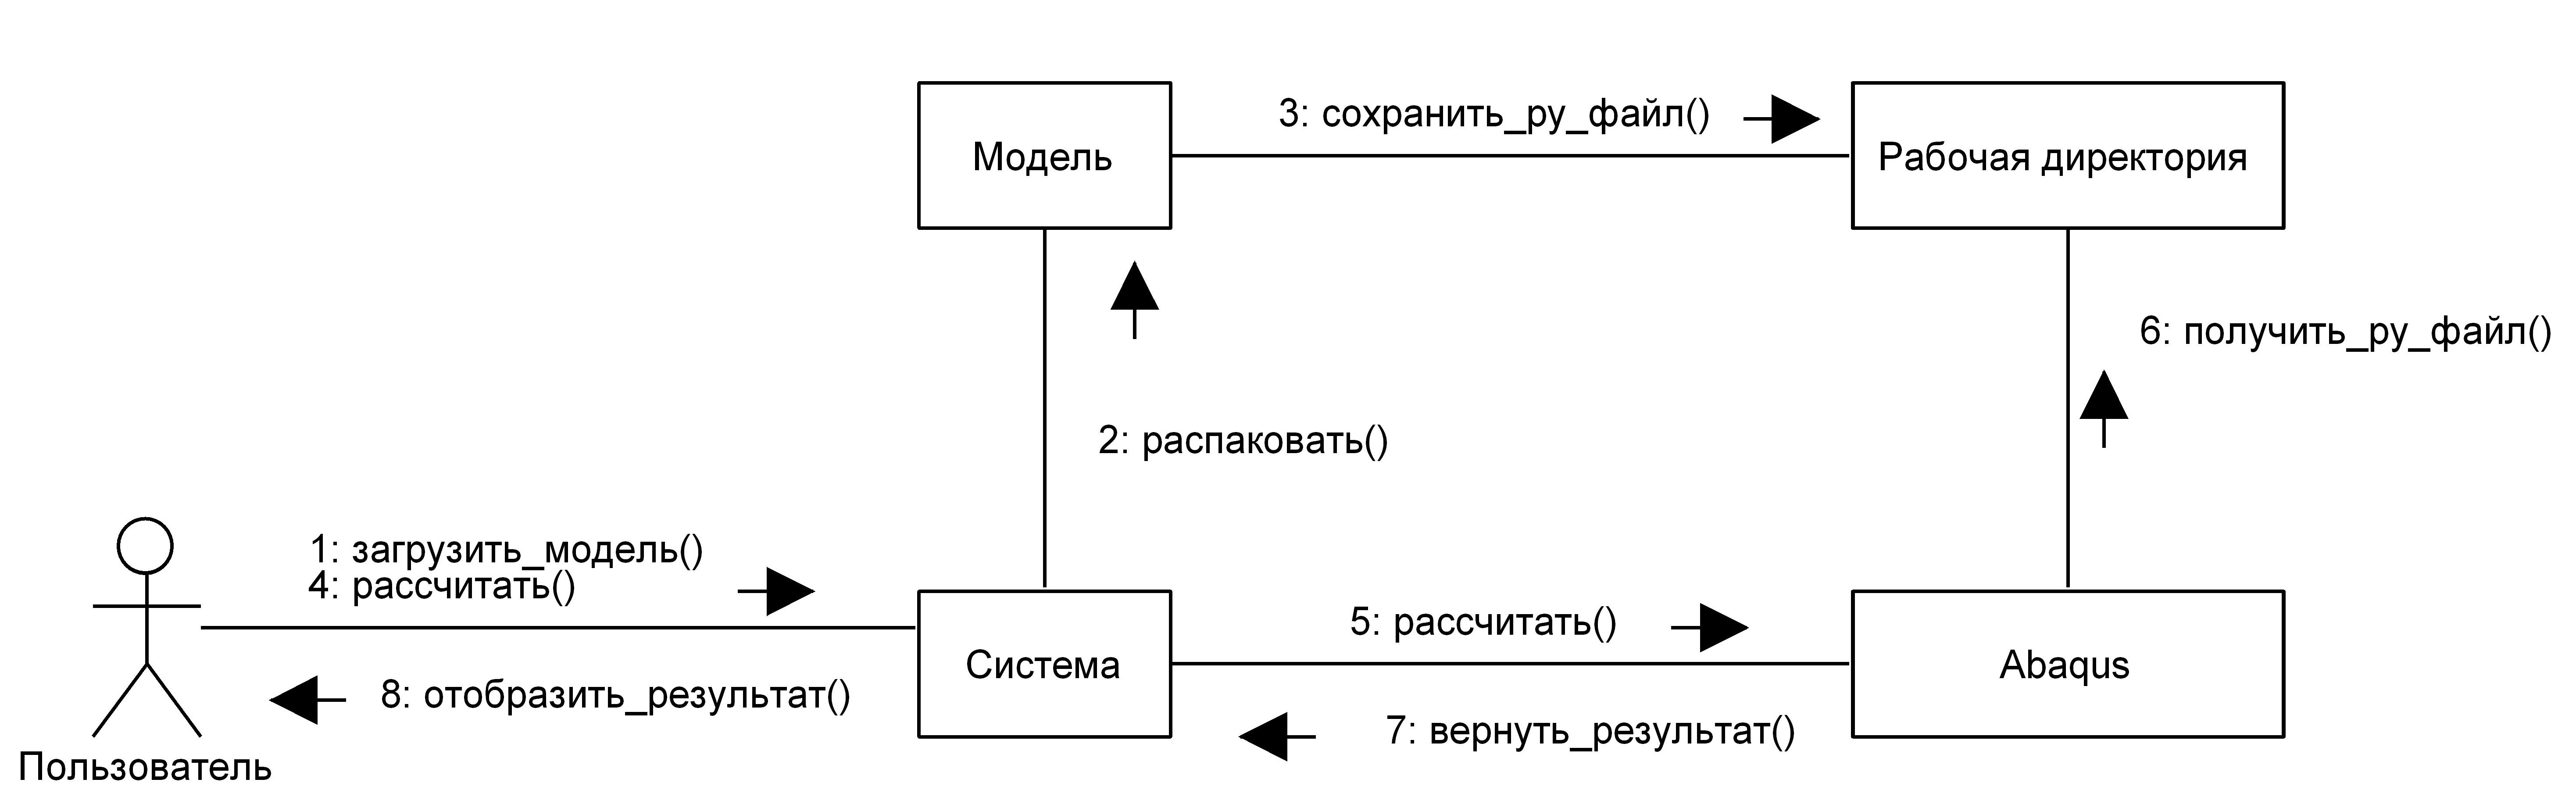
\includegraphics[width=1\textwidth]{img/commun-diagram} 
		\end{center}
		\caption{Диаграмма взаимодействия}
		\label{fig:commun-diagram}
	\end{figure}
	
	На рисунке \ref{fig:commun-diagram} показана UML диаграмма коммуникаций относительно вызова выполнения расчетного сценария. Как показано на диаграмме, после инициирования пользователем загрузки модели в систему, модель распаковывается в виде .py файла в текущую рабочую директорию. Таким образом, когда пользователь инициирует расчет модели, система поддержки выбора режимов резания вызывает Abaqus через командную строку с указанием предварительно распакованного файла сценария.
	
	Отдельно стоит отметить, что модуль выполнения Abaqus скриптов слабо связан с основной системой. Такой эффект достигается благодаря декларированию обобщенного интерфейса запуска любых скриптов. В терминологии NetBeans платформы этот интерфейс называется сервисом. Конкретный класс сервиса не известен до момента выполнения программы. Если реализовать интерфейс запуска в соответствии с особенностями другой CAE системы, отличной от Abaqus, то этот новый модуль также сможет работать в составе системы. 
	
	
	\section{Отображение графиков}	
	По результатам моделирования требуется предоставить пользователю информацию о возникающих деформациях. Эта задача решается при помощи модуля построения графиков. Перед завершением своей работы, Python сценарий сохраняет информацию о узловых перемещениях в текстовый обменный файл. Благодаря этому файлу становится возможно отображение требуемых графиков по точкам в интегрированной системе поддержки принятия решения.
	
	Структура обменного текстового файла проста и соответствует стандартному формату экспорта точек из Abaqus. Ниже приведен фрагмент файла. 
	\begin{lstlisting}[style=nonumbers]
	X              XYData-1
	
	0.00000E+000   7.12293E-004
	2.09397E-003   6.84344E-004
	4.18794E-003   6.29122E-004
	6.28191E-003   5.48125E-004
	... 		   ...
	\end{lstlisting}
	В левой колонке записаны координаты текущей точки в естественной системе координат. В правой -- значения узловых перемещений для заданной координаты.
	
	\begin{figure}[!h]
		\begin{center}
			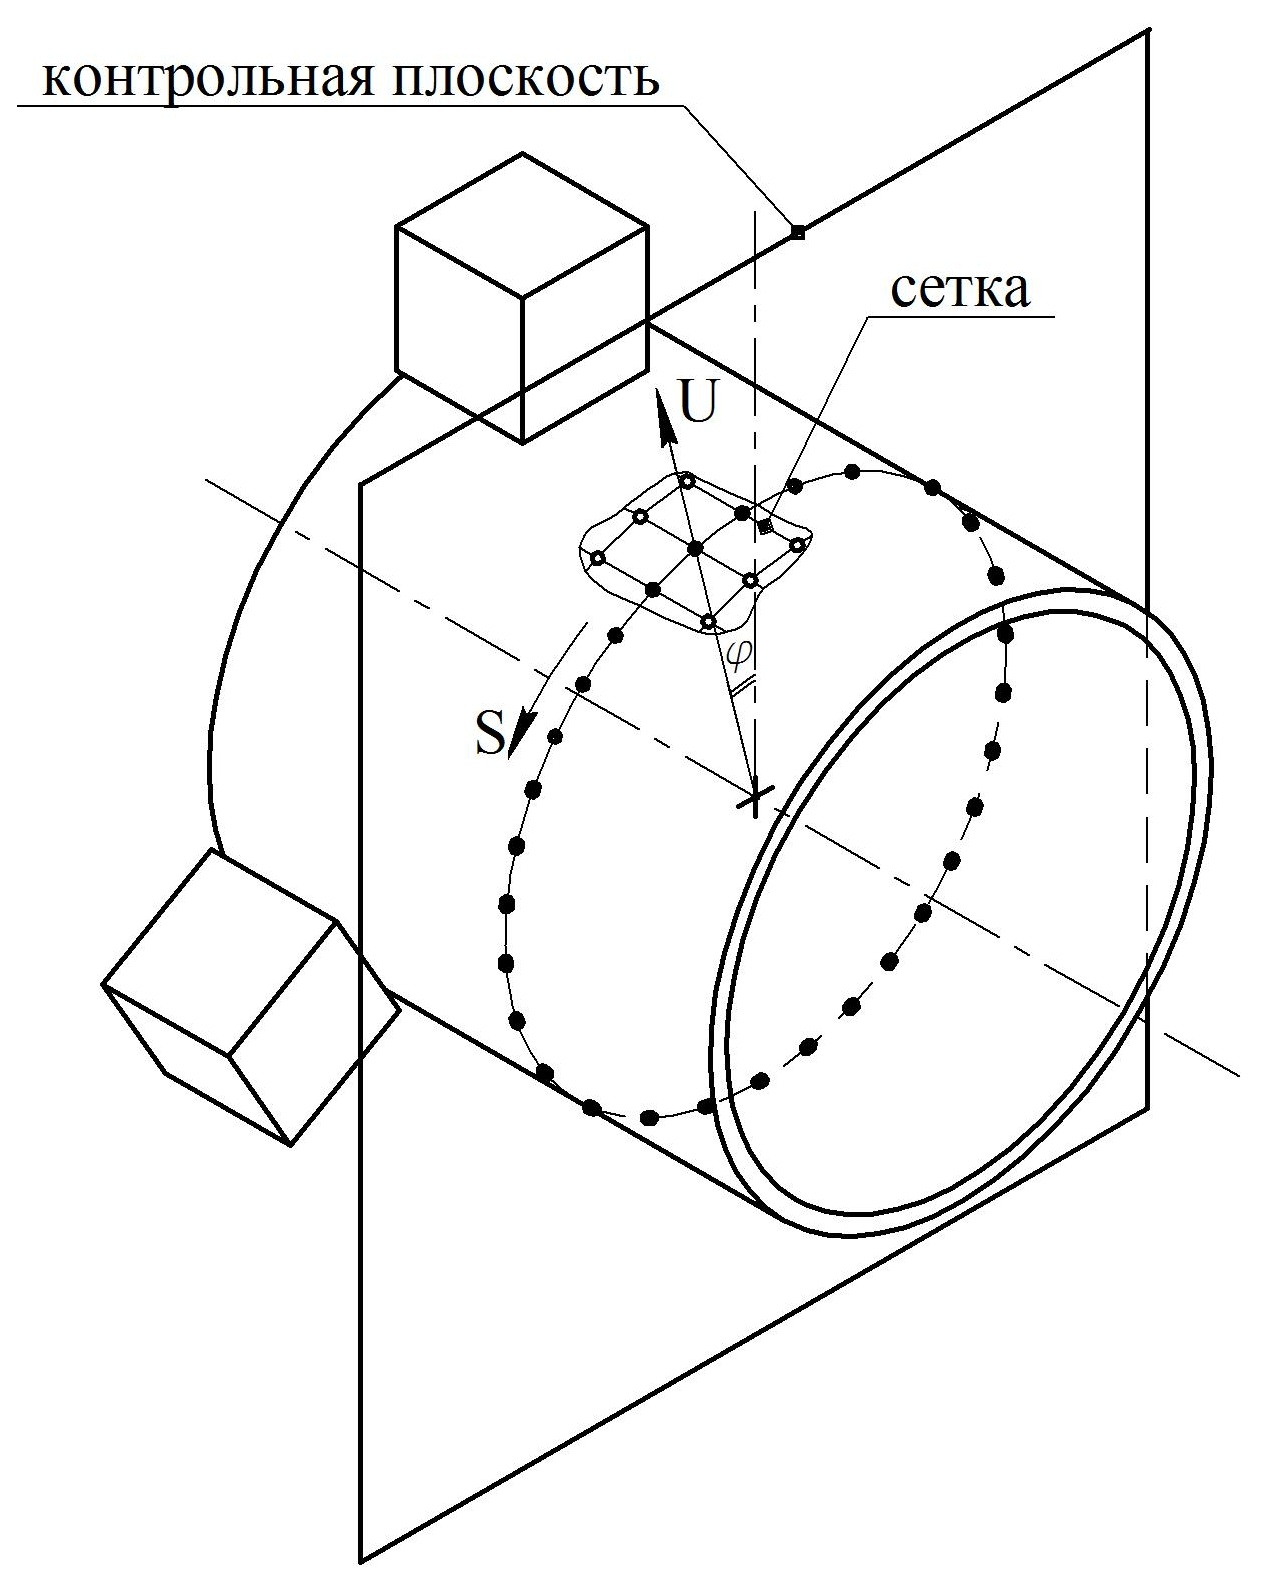
\includegraphics[scale=1]{img/control-plane} 
		\end{center}
		\caption{Схема расположения контрольных точек}
		\label{fig:control-plane}
	\end{figure}
		
	Схема расположения контрольных точек приведена на рисунке \ref{fig:control-plane}. В обменном файле сохранены естественные координаты точек (S,U), которые необходимо преобразовать в полярные ($ \mathrm{\varphi} $, U).
	
	
	\begin{figure}[t!]
		\centering	
		\noindent
		\begin{minipage}[b!]{0.5\textwidth}
			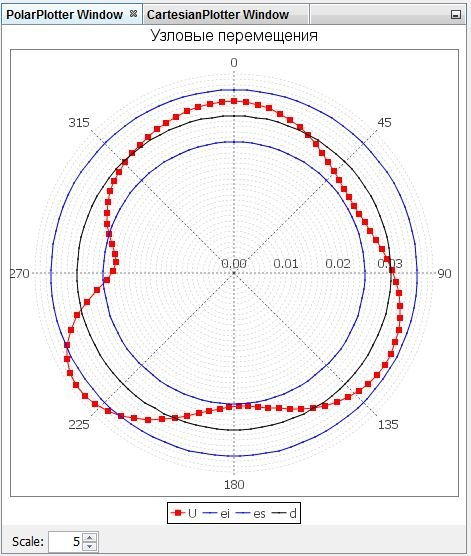
\includegraphics[width=0.97\textwidth]{img/graph-screen} 
			\caption{Полярный график}
			\label{fig:graph-screen}
		\end{minipage}%
		\begin{minipage}[b!]{0.5\textwidth}
			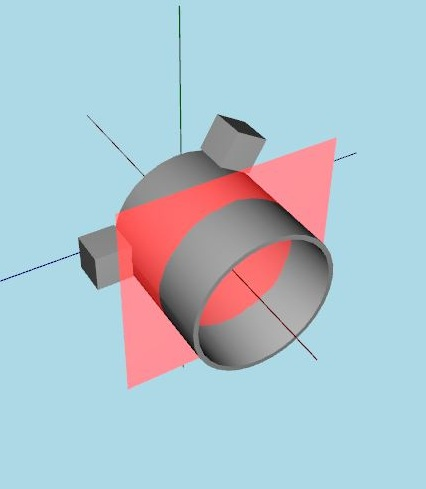
\includegraphics[width=0.99\textwidth]{img/viewport-screen2} 
			\caption{Контрольная плоскость}
			\label{fig:viewport-screen2}	
		\end{minipage}
	\end{figure}
	
	После преобразования координат производится построение графика средствами Java библиотеки JFreeChart (изображено на рисунке \ref{fig:graph-screen}). Следует отметить, что пользователь может вручную задать  положение контрольной плоскости по расстоянию до торца заготовки. На рисунке  \ref{fig:viewport-screen2} показано произвольное положение красной контрольной плоскости. Контрольная плоскость определяет положение точек, используемых для построения графиков (показаны черными на рисунке \ref{fig:control-plane}). Эти точки находятся в узлах МКЭ сетки. 
	
	
	\begin{figure}[b!]
		\centering	
		\noindent
		\begin{minipage}[b!]{0.55\textwidth}
			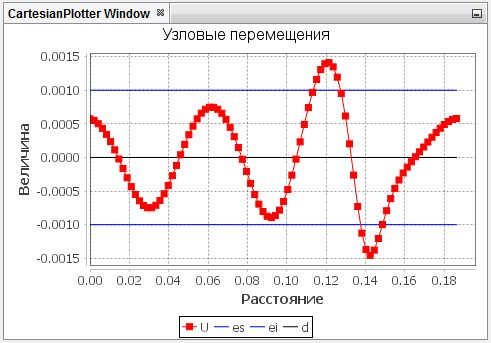
\includegraphics[width=0.99\textwidth]{img/cartesian-graph} 
			\caption{График в декартовых координатах}
			\label{fig:cartesian-graph}
		\end{minipage}%
		\begin{minipage}[b!]{0.45\textwidth}
			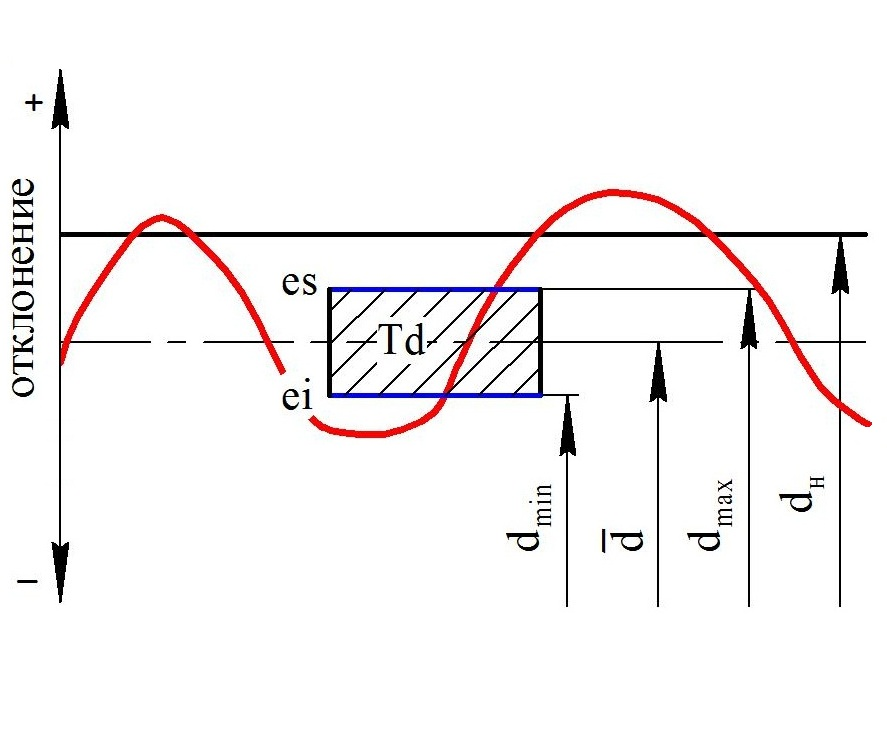
\includegraphics[width=0.99\textwidth]{img/tolerance} 
			\caption{Схема построения графиков}
			\label{fig:tolerance}	
		\end{minipage}
	\end{figure}
	
	Система поддерживает построение двух типов графиков: в полярных и декартовых координатах. На рисунке \ref{fig:graph-screen} показан график в полярных координатах, а соответствующий ему график в декартовых координатах -- на рисунке \ref{fig:cartesian-graph}.
		

	Принцип построения графика показан на рисунке \ref{fig:tolerance}. Красной линией на график наносится значения узловых перемещений в каждой контрольной точке. За начало отчета принято недеформированное состояние детали, которое совпадает со средним значением диаметра $ \overline{d} $ в идеальном случае. Синими линиями показаны верхнее es и нижнее ei отклонения. Номинальный диаметр $ d_{\textup{ном}} $ на графике не отображается.
	
	Задача пользователя состоит в том, чтобы подобрать режимы резания таким образом, чтобы красный график находился между синими линиями и не пересекал их. В этом случае узловые перемещения не превышают допуска. 
		
	\chapter{Рабочее проектирование}
	\section{Испытание калькулятора режимов резания}
	\subsection{Методика испытания}
	Калькулятор режимов резания будет испытан по трем произвольным расчетным случаям. Для каждого расчетного случая будет определены режимы резания вручную по таблично-аналитической методике, приведенной в \cite{book:Kosilova} и при помощи разработанного модуля. Относительная погрешность не должна составлять более 10\%. Исходные данные для испытаний приведены в таблице \ref{tab:test-data}.
	
	\begin{table}[h!]
		\centering
		\caption{Исходные данные}
		\label{tab:test-data}	
	\begin{tabular}[h!]{ |  >{\centering\arraybackslash} m{4.5cm}|  >{\centering\arraybackslash} m{3.6cm}|  >{\centering\arraybackslash} m{3.6cm}|  >{\centering\arraybackslash} m{3.6cm}|}
		\hline
		Расчетный случай           &  \rom{1}  &   \rom{2}    &  \rom{3}   \\ \hline
		Диаметр поверхности, мм    &    30     &       45     &    60      \\ \hline
		Тип точения                & черновое  & получистовое & чистовое   \\ \hline
		Вид обработки	           &вн. точение& вн. точение  &растачивание\\ \hline
		Материал заготовки         &   сталь   &     чугн     &  чугн      \\ \hline
		Вид заготовки              &  поковка  &   отливка    &  прокат    \\ \hline
		Материал инструмента       &  Т15К6    &     ВК6      &   ВК8      \\ \hline
		Период стойкости резца, мин&   30      &    40        &   60       \\ \hline
		Шероховатость поверхности  &   3,2     &    2,5       &   1,25     \\ \hline	
		Радиус при вершине резца   &   0,75    &     1,5      &    4       \\ \hline					
	\end{tabular}
	\end{table}
	
	\subsection{Расчет режимов резания}
	Расчетный случай \rom{1} будет рассмотрен подробно, для остальных приведены только результаты. Получаемые значения вычисляемых величин зависят от  глубины резания $ t $, назначенной произвольно в ограниченном диапазоне, поэтому значение глубины резания будет принято в соответствии с запрограммированным алгоритмом. Согласно выбранной методике, глубина резания для шероховатости Ra=3,2 мм принимается из диапазона $ t=0,5\div2,0 \textup{мм} $. Для данного случая алгоритмом получено допустимое значение $ t=1,05 \textup{ мм} $, которое будет дальше использоваться в аналитических расчетах. 
	
	По таблице 11, приведенной в \cite{book:Kosilova}, для чернового наружного точения при $ t<3 \textup{ мм} $ подача назначается из диапазона $ 0,4-0,5 \textup{ мм/об} $. Примем $ s=0,45 \textup{ мм/об} $.
	
	Скорость резания определяется по эмпирической формуле
	\[ v=\frac{C_v}{T^mt^xs^y}K_v, \:\textup{м/мин} \]
	где $ C_v,m,x,y $~--~эмпирические коэффициенты;\\
	\phantom{где\space} $ T $~--~период стойкости резца, мин;\\
	\phantom{где\space} $ t $~--~глубина резания, мм;\\
	\phantom{где\space} $ s $~--~подача, мм/об;\\
	\phantom{где\space} $ K_v $~--~поправочный коэффициент, мм/об;\\
	По таблице 17 из \cite{book:Kosilova} для случая обработки конструкционной стали резцом с режущей частью из твердого сплава Т15К6 и подачи \mbox{ $ 0,3<s<0,7 \textup{ мм/об} $}, значения эмпирических коэффициентов равны: $ C_v=350 $, $  x=0,15 $, $  y=0,35 $, $  m=0,20 $. Период стойкости резца задан $ T= 30 \textup{ мин} $. Коэффициент $ K_v $ является произведением коэффициентов, учитывающих влияние материала заготовки $ K_\textup{МV}=1,25 $, состояния поверхности $ K_\textup{ПV}=0,8 $ (для поковки) и материала инструмента $ K_\textup{ИV}= 1 $ (для твердого сплава Т15К6). При подстановке определенных коэффициентов в формулу для вычисления скорости резания, получим:
	\[ v=\frac{350}{30^{0,20} \cdot 1,05^{0,15} \cdot 0,45^{0,35}} \cdot 1,25 \cdot 0,8 \cdot 1 = 232,720 \textup{ м/мин} \]
	Частота вращения заготовки вычисляется следующим образом:	
	\[ n= \frac{1000 \cdot v}{\pi D} = \frac{1000 \cdot 232,720}{\pi \cdot 30} = 2469,277  \textup{ об/мин}  \]
	где $ v $~--~скорость резания м/мин;\\
	\phantom{где\space} $ D $~--~диаметр заготовки, мм;\\
	Сила резания может быть получена из формулы 
	\[  P_z=10\cdot C_p\,t^x\,s^y\,v^n\,K_{P}, \textup{ Н}    \]
	где $ C_p,x,y,n $~--~табличные коэффициенты;\\
	\phantom{где\space} $ t $~--~глубина резания, мм;\\
	\phantom{где\space} $ s $~--~подача, мм/об;\\
	\phantom{где\space}	$ v $~--~скорость резания м/мин;\\
	\phantom{где\space} $ K_P $~--~поправочный коэффициент, мм/об;\\	
	По таблице 22, приведенной в литературе \cite{book:Kosilova} для стальной заготовки, резца из твердого сплава и наружного точения  могут быть определены следующие значения коэффициентов $ C_p=300,\:x=1,\:y=0,75,\:n=-0,15 $. Поправка на материал заготовки $ K_P =0,91$

	После подстановки получаем значение силы резания: 
	\[  P_z=10\cdot 300 \cdot 1,05^1 \cdot 0,45^{0,75} \cdot 2469.277^{-0,15} \cdot 0,91 = 487,951 \textup{ Н}    \]
	Момент резания может быть вычислен исходя из полученной силы резания $ P_z $ и известного диаметра заготовки $ D $: $ M= \dfrac{P_zD}{2000} = 7,319  \textup{ Нм} $. Потребляемая мощность также определяется исходя из рассчитанных значений: $ N= \dfrac{P_zv}{1020 \cdot 60	} = 1,856  \textup{ кВт} $.
	
	Вся информация по результатам сведена в таблицу \ref{tab:tests}. Исходя из таблицы видно, что методика расчета режимов резания реализована в расчетном модуле без ошибок. Глубина резания и подача выбирается из таблиц корректно, поэтому для этих величин отсутствует погрешность. Погрешность остальных величин объясняется обобщением эмпирических коэффициентов при  их приведении к нормализованному виду для записи в базу знаний.

	\begin{table}[]
		\centering
		\caption{Сводная таблица испытаний}
		\label{tab:tests}
		\scalebox{0.84}{
		\begin{tabular}{|c|l|c|c|c|c|c|c|c|}
			\hline
			\multicolumn{2}{|l|}{Величина}    		& \multicolumn{1}{l|}{\begin{tabular}[c]{@{}l@{}}Глубина \\ резания \\ $ t $, мм\end{tabular}} & \multicolumn{1}{l|}{\begin{tabular}[c]{@{}l@{}}Подача \\ $ s $, мм/об\end{tabular}} & \multicolumn{1}{l|}{\begin{tabular}[c]{@{}l@{}}Скорость\\ резания \\ $ v $, м/мин\end{tabular}} & \multicolumn{1}{l|}{\begin{tabular}[c]{@{}l@{}}Сила \\ резания \\ $ P_z $, Н\end{tabular}} & \multicolumn{1}{l|}{\begin{tabular}[c]{@{}l@{}}Момент \\ резания \\ $ P_z $, Н\end{tabular}} & \multicolumn{1}{l|}{\begin{tabular}[c]{@{}l@{}}Потребляемая \\ мощность \\ $ N $, кВт\end{tabular}} & \multicolumn{1}{l|}{\begin{tabular}[c]{@{}l@{}}Частота \\ вращения \\ $ n $, об/мин\end{tabular}} \\ \hline
			\multirow{3}{*}{I}     & К              & $ 1,05 $                                                                                     & $ 0,45 $                                                                            & $ 232,610 $                                                                                     & $508,857 $                                                                                 & $7,633$                                                                                      & $1,934$                                                                                             & $2468,073 $                                                                                       \\ \cline{2-9} 
								   & Т-А            & $ 1,05 $                                                                                     & $ 0,45 $                                                                            & $ 232,720 $                                                                                     & $487,957 $                                                                                 & $7,319$                                                                                      & $1,856$                                                                                             & $2468,277$                                                                                        \\ \cline{2-9} 
							       & $ \delta, \% $ & $ 0 $                                                                                   	   & $ 0 $                                                                               & $ -0,04 $                                                                                       & $4,28    $                                                                                 & $4,29$                                                                                       & $4,20$                                                                                              & $ \approx 0 $                                                                                     \\ \hline
			\multirow{3}{*}{II}    & К              & $ 0,85 $                                                                                     & $ 0,20 $                                                                            & $ 168,367 $                                                                                     & $252,414 $                                                                                 & $5,679$                                                                                      & $0,694$                                                                                             & $1190,949$                                                                                        \\ \cline{2-9} 
								   & Т-А            & $ 0,85 $                                                                                     & $ 0,20 $                                                                            & $ 168,596 $                                                                                     & $234,456 $                                                                                 & $5,531$                                                                                      & $0,682$                                                                                             & $1190,031$                                                                                        \\ \cline{2-9} 
								   & $ \delta, \% $ & $ 0 $                                                                                        & $ 0 $                                                                               & $ 0,13 $	                                                                                       & $7,66    $                                                                                 & $2,67$                                                                                       & $1,76$                                                                                              & $0,07$                                                                                            \\ \hline
			\multirow{3}{*}{III}   & К              & $ 0,85 $                                                                                     & $ 0,14 $                                                                            & $ 157,120 $                                                                                     & $192,396 $                                                                                 & $5,772$                                                                                      & $0,494$                                                                                             & $ 833,547 $                                                                                       \\ \cline{2-9} 
								   & Т-А            & $ 0,85 $                                                                                     & $ 0,14 $                                                                            & $ 156,989 $                                                                                     & $187,917 $                                                                                 & $5,471$                                                                                      & $0,471$                                                                                             & $ 833,497 $                                                                                       \\ \cline{2-9} 
								   & $ \delta, \% $ & $ 0 $                                                                                        & $ 0 $                                                                               & $ -0,08 $                                                                                       & $2,38 $                                                                                    & $5,48$                                                                                       & $4,88$                                                                                              & $ \approx 0 $                                                                                     \\ \hline
		\end{tabular}
	}
	\end{table}

	
	\section{Испытание загрузчика моделей}
	\subsection{Методика испытания}
	Загрузчик моделей испытывается на нескольких произвольных пробных моделях. Контролируется корректность отображаемой геометрии в модуле визуализации, а также правильность построения иерархии параметров.

	\subsection{Проведение испытаний}
	Для проверки работоспособности загрузчика были составлены три модели произвольной геометрии. В данном случае испытания не предполагают полную параметризацию геометрии, поэтому для тестовых моделей она задана однозначно. Результат загрузки показан в таблице \ref{tab:loader-tests}.   
	
	Из таблицы видно, что все модели отображаются в соответствии с построениями в Abaqus и модуль загрузки реализован без ошибок.
	
	\begin{table}[]
		\centering
		\caption{Испытание загрузчика}
		\label{tab:loader-tests}{
		{\tabulinesep=1.2mm
		\begin{tabu}[]{|c|c|}
				\hline
				Загруженная модель 							   & Модель в Abaqus  \\
				\hline
				\rule{0pt}{4ex} 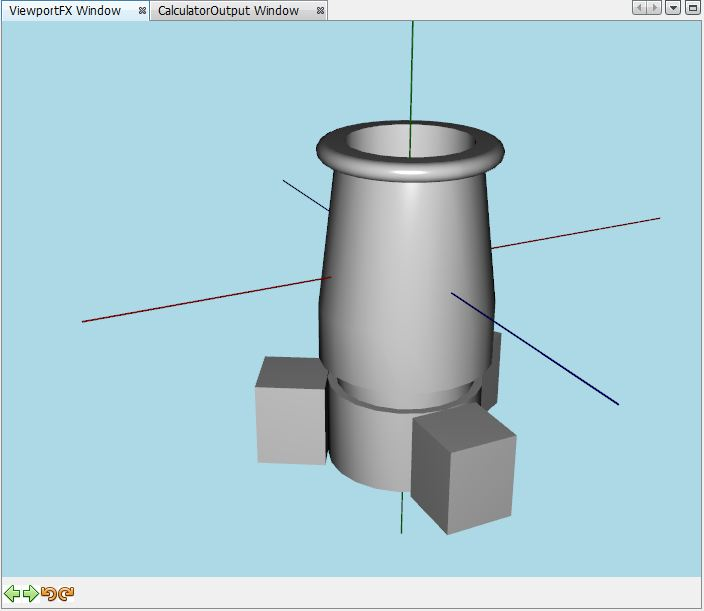
\includegraphics[scale=0.40]{img/loader-test1} & 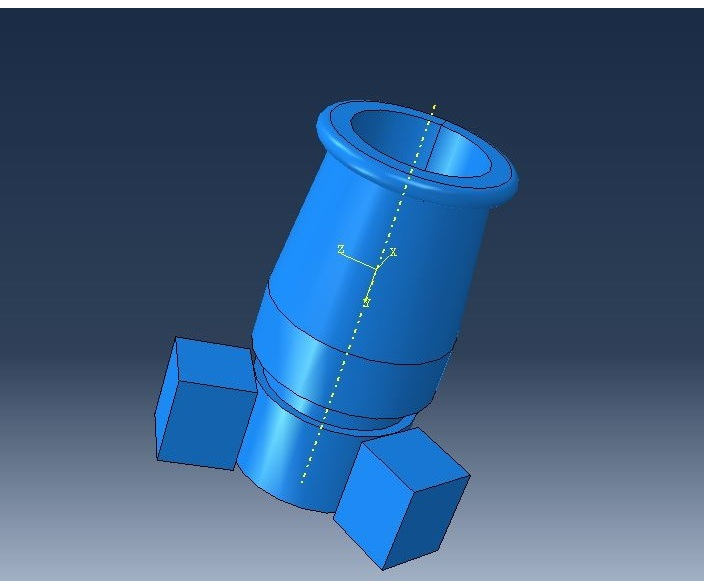
\includegraphics[scale=0.43]{img/loader-test1-abq}  \\ 
				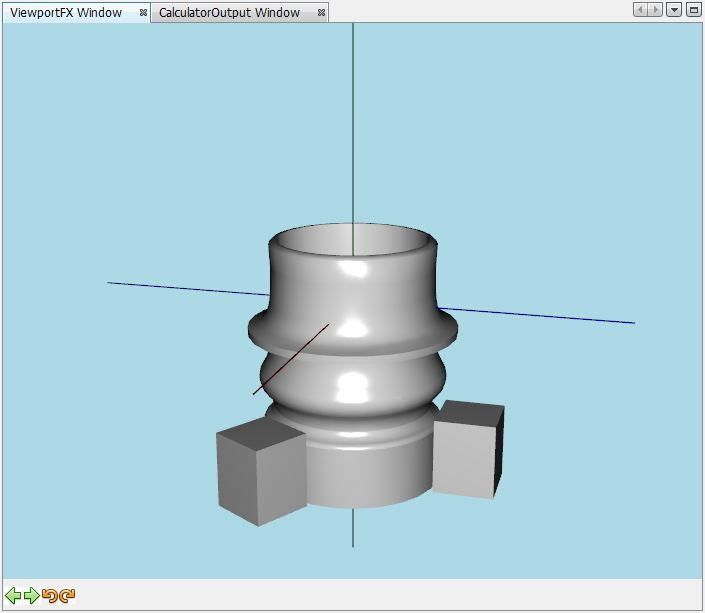
\includegraphics[scale=0.40]{img/loader-test2} & 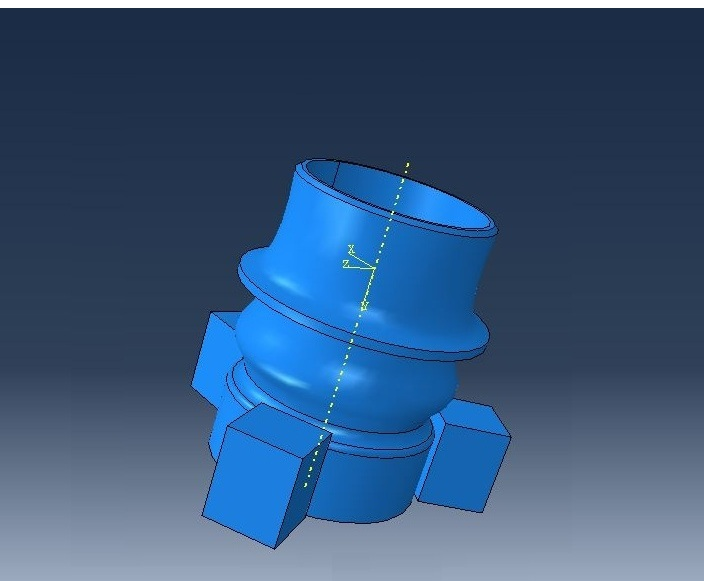
\includegraphics[scale=0.43]{img/loader-test2-abq} \\ 
				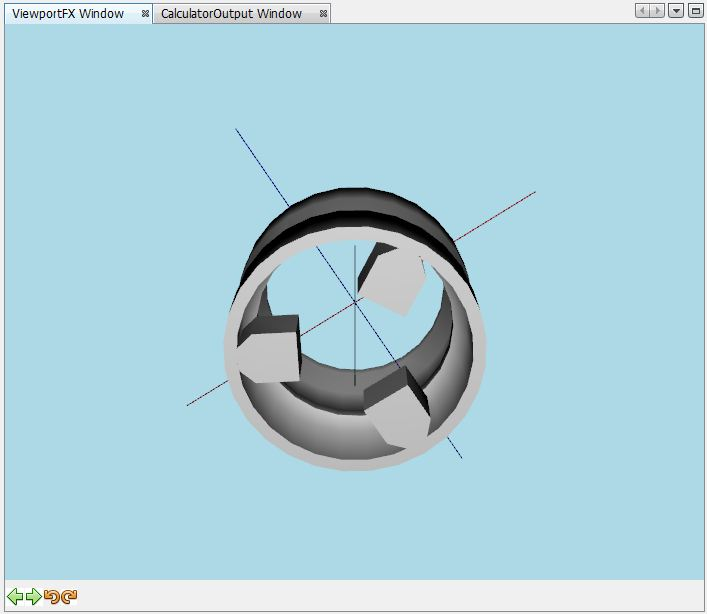
\includegraphics[scale=0.40]{img/loader-test3} & 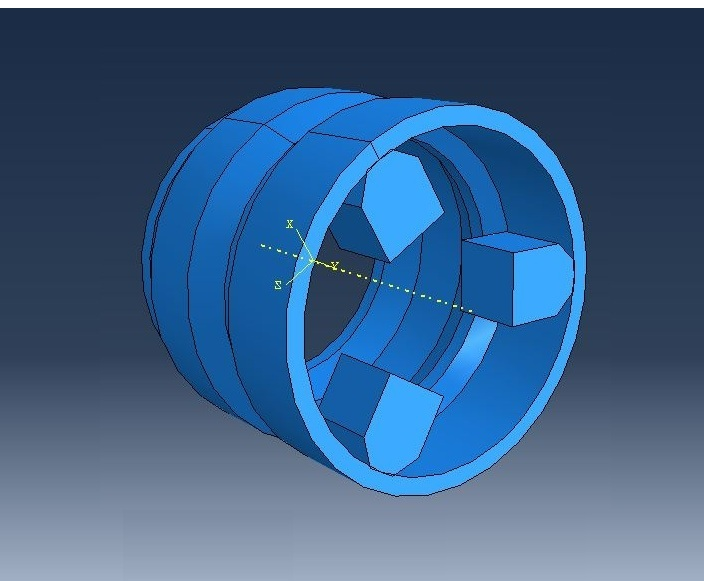
\includegraphics[scale=0.43]{img/loader-test3-abq} \\ 
				\hline
		\end{tabu}
		}
	}\end{table}
	
	Для проверки правильности загрузки дерева параметров составлена пробная модель по схеме на рисунке \ref{fig:model-tree-abstract}. Как видно из рисунка \ref{fig:loader-tree-test}, произвольное дерево параметров загружается в систему в соответствии с записанной в файл структурой.
	
	\begin{figure}[!h]
		\begin{center}
			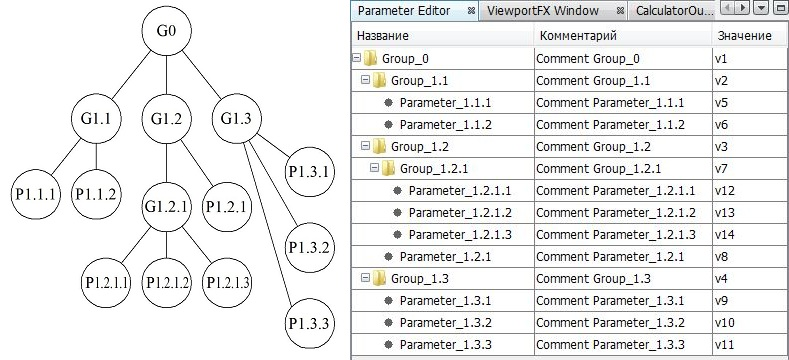
\includegraphics[width=\textwidth]{img/loader-tree-test} 
		\end{center}
		\caption{Испытание загрузки дерева параметров}
		\label{fig:loader-tree-test}
	\end{figure}
	
	\section{Испытание подсистемы параметризации}
	\subsection{Методика испытания}
	Под системой параметризации понимается функционал разработанного ПО, отвечающий за применение действительных значений параметров к модели. Контролю подлежат прежде всего геометрические параметры, такие как длина заготовки, наружный и внешние диаметры. Для контролируемых параметров выставляют несколько различных значений и проверяют правильность изменения 3D модели. Например, при увеличении длины заготовки в редакторе параметров, соответствующее изменение должно быть отображено в модуле визуализации после обновления модели. 
	
	\begin{table}[]
		\centering
		\caption{Испытание подсистемы параметризации}
		\label{tab:param-tests}{
			\scalebox{0.9}{
				{\tabulinesep=1.2mm
					\begin{tabu}[]{|c|c|}
						\hline
						$ l = 0,02 $ & $ l = 0,06 $ \\
						\hline
						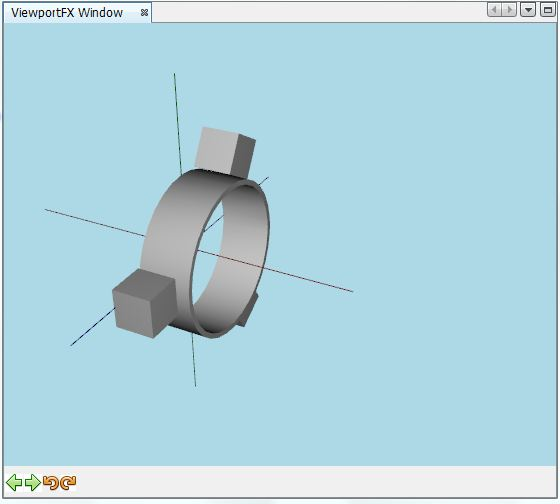
\includegraphics[scale=0.55]{img/length-test1} & 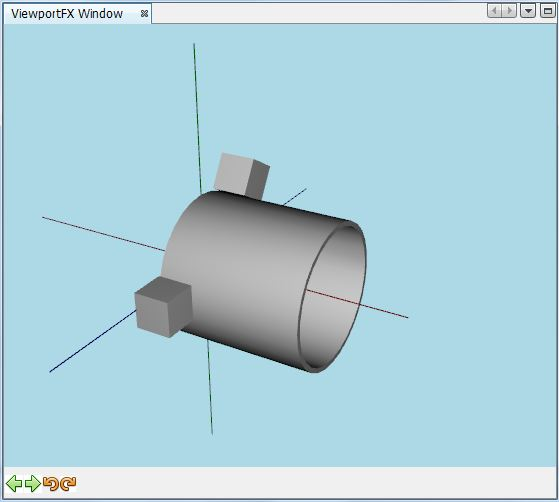
\includegraphics[scale=0.55]{img/length-test2}  \\ 
						\hline
						$ l = 0,12 $ & $ d_\textup{внутр} = 0,0295 $ \\
						\hline
						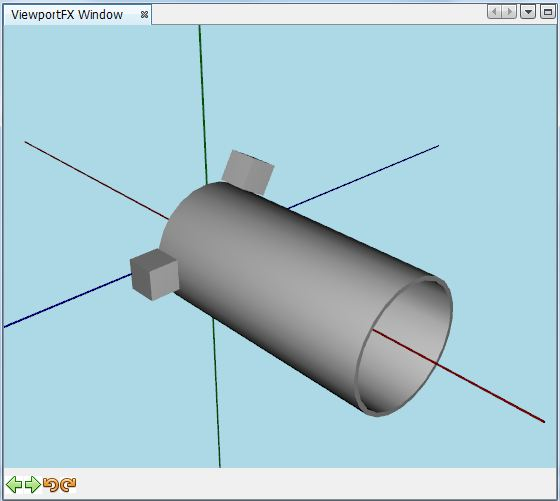
\includegraphics[scale=0.55]{img/length-test3} & 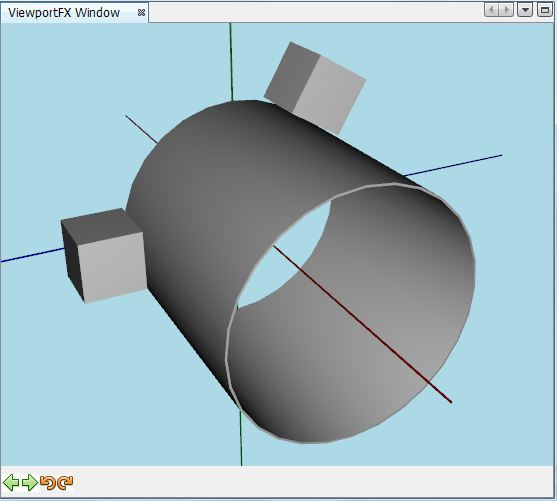
\includegraphics[scale=0.55]{img/diam-test1}  \\ 
						\hline
						$  d_\textup{внутр} = 0,025 $ & $ d_\textup{внутр} = 0,020 $ \\
						\hline
						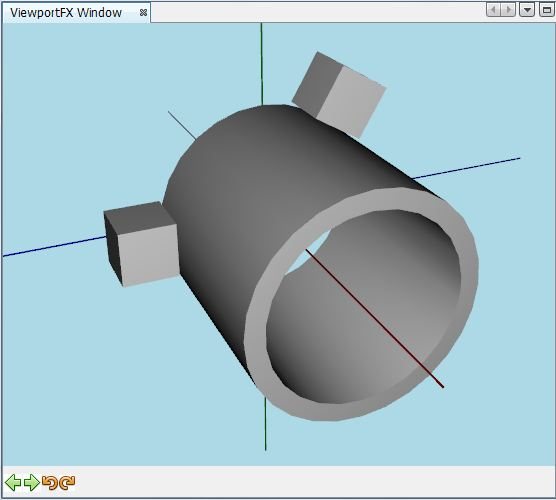
\includegraphics[scale=0.55]{img/diam-test2} & 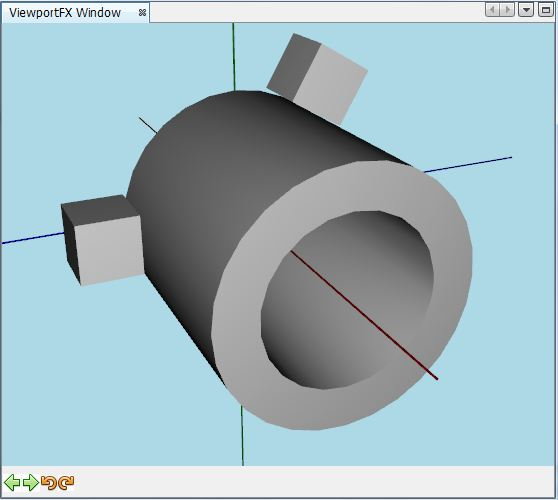
\includegraphics[scale=0.55]{img/diam-test3}  \\ 
						\hline
					\end{tabu}
				}
			}
		}\end{table}	
	
	\subsection{Проведение испытаний}	
	В таблице \ref{tab:param-tests} приведены результаты испытаний для трех, выбранных произвольно, значений длины заготовки $ l=0,02;\:0,06;\:0,12 \textup{ м} $ и внутреннего диаметра $ d_\textup{внутр}=0,0295;\:0,025;\:0,020 \textup{ м} $. Все приведенные параметры модели применяются корректно, происходит обновление изображения заготовки в окне визуализации, следовательно, подсистема параметризации реализована правильно.
	
	\section{Испытание подсистемы моделирования}
	\subsection{Методика испытания}
	При испытаниях подсистемы моделирования необходимо проконтролировать следующие положения:
	\begin{itemize}
		\item Зависимость результата моделирования от величины силы резания и её положения
		\item Зависимость картины деформации от числа кулачков
		\item Зависимость величины узловых перемещений от смещения кулачков
		\item Изменение графиков узловых перемещений в зависимости параметров модели
		\item Изменение графиков узловых перемещений в зависимости от положения контрольной плоскости
		\item Возможность моделирования произвольного расчетного случая
	\end{itemize}
	
	Указанные положения проверяются соответствующими изменениями параметров модели по нескольким произвольным значениям. 
	

	\newpage
	\subsection{Проведение испытаний}	
	В таблице 10 продемонстрирована возможность изменять количество кулачков. Соответствующие графики отображают изменения числа кулачков. Результаты испытаний для остальных контролируемых положений приведены в приложении \ref{app:testing}. Например, в таблице \ref{tab:displ-tests} показано изменение величины узловых перемещений при увеличении смещения кулачков. Результаты работы программы подтверждают ожидания: в этом случае узловые перемещения увеличиваются. Таблица \ref{tab:modeling-force-tests} демонстрирует проверку различных значений силы резания и угла точки приложения. 
	
		\begin{table}[]
			\centering
			\caption{Испытание подсистемы моделирования: число кулачков}
			\label{tab:modeling-tests}{
				{\tabulinesep=1.2mm
					\begin{tabu}[]{|c|c|}
						\hline
						\multicolumn{2}{|c|}{$ n_\textup{кулачков}=4 $} \\ \hline
						\includegraphics[scale=0.55]{img/simulation-jaw-test-model1} & \includegraphics[scale=0.55]{img/simulation-jaw-test-graph1}  \\ 
						\hline
						\multicolumn{2}{|c|}{$ n_\textup{кулачков}=6 $} \\ \hline
						\includegraphics[scale=0.55]{img/simulation-jaw-test-model2} & \includegraphics[scale=0.55]{img/simulation-jaw-test-graph2}  \\ 
						\hline
					\end{tabu}
				}
			}\end{table}


	\chapter{Расчет затрат на разработку интегрированной системы поддержки принятия решения}
	\section{Введение}
	В данной главе сформулированы этапы разработки, произведен расчёт трудоемкости, установлен состав исполнителей, определена продолжительность выполнения отдельных этапов и вычислены затраты на создание системы поддержки принятия решения.	
	
	\section{Организация и планирование процесса разработки}
	Разработка интегрированной системы поддержки принятия решения является сложным процессом, стадии которого определяются ГОСТом Единой Системы Программной Документации \cite{gost:19102}. Согласно указанному документу всего выделяется 5 стадий, их подробное описание приведено в таблице \ref{tab:economy}.
	
	Основными факторами, определяющими трудоемкость создания интегрированной системы являются: степень новизны разрабатываемого программного комплекса, сложность алгоритма его функционирования, объем используемой информации, вид её представления и способ обработки, уровень языка программирования \cite{metoda:Economy}. Определим принадлежность разрабатываемого продукта к группам по каждому из указанных факторов. 
	
	По степени новизны интегрированная система может быть отнесена к группе <<Б>>: она не имеет аналогов, но и не требует разработки принципиально новых методов создания. 
	
	По степени сложности систему можно отнести к группе продукции, реализующей алгоритмы стандартных методов 
	решения задач, то есть к группе 3. Непосредственная реализация метода конечных элементов не входит в рамки разработки продукта, а включение модуля оптимизации в состав системы  на текущем этапе не предполагается.  \newpage

		\begin{table}[h!]
			\centering
			\caption{Стадии разработки}\label{tab:economy} 
			\begin{tabularx}{\textwidth}{|l|X|}
				
				\hline Стадия разработки & \multicolumn{1}{Z|}{Состав выполняемых работ }\\ 
				\hline Техническое задание & Постановка задач, выбор критериев эффективности. Разработка технико-экономического обоснования разработки. Предварительный выбор методов выполнения работы. Разработка календарного плана выполнения работ   \\ 
				\hline Эскизный проект & Предварительная разработка структуры входных и выходных данных. Разработка общего описания алгоритмов реализации решения задач. Разработка пояснительной записки. Согласование и утверждение эскизного проекта \\ 
				\hline Технический проект & Разработка алгоритмов решения задач. Разработка пояснительной записки. Согласование и утверждение технического проекта. Уточнение структуры, анализ и определение формы представления входных и выходных данных. Выбор конфигурации технических средств.  \\ 			
				\hline Рабочий проект & Комплексная отладка и сдача в опытную эксплуатацию. Разработка проектной документации. Разработка, согласование программы и методики испытаний. Предварительное проведение всех видов  испытаний.   \\ 			
				\hline Внедрение & Подготовка и передача программной документации для сопровождения с оформлением соответствующего акта. Передача программной продукции в фонд алгоритмов и программ. Проверка алгоритмов и программ решения задач, корректировка документации после опытной эксплуатации программного продукта. \\ 
				\hline 
			\end{tabularx}
		\end{table}
		
		
	Как показал анализ литературы \cite{book:Kosilova}, исходная информация представлена как в виде формул, так и в виде разнородных таблиц. При этом требуется учитывать взаимное влияние данных, содержащихся в этих таблицах. Таким образом, разрабатываемую программу по виду представления исходной информации относят к группе 11. По структуре выходных документов система принадлежит группе 22 - требуется вывод на печать одинаковых документов, представляющих собой отчеты о моделировании.
	
	\section{Расчет трудоемкости этапов} 
	\subsection{Расчет трудоемкости разработки технического задания}
	Трудоемкость разработки технического задания может быть рассчитана по формуле:
	\begin{equation}\label{eq:TZ}
		\tau_\textup{\scriptsize{ТЗ}} = T^{\textup{\scriptsize{З}}}_\textup{\scriptsize{РЗ}} + T^{\textup{\scriptsize{З}}}_\textup{\scriptsize{РП}},	
	\end{equation} 
	где	$\tau_\textup{\scriptsize{ТЗ}}$~--~трудоемкость разработки технического задания на создание программного продукта, \mbox{чел.-дни};\newline
	\phantom{где\space}$T^{\textup{\scriptsize{З}}}_\textup{\scriptsize{РЗ}}$~--~затраты времени разработчика постановки задачи на разработку ТЗ, \mbox{чел.-дни};\newline
	\phantom{где\space}$T^{\textup{\scriptsize{З}}}_\textup{\scriptsize{РП}}$~--~затраты времени разработчика программного обеспечения на разработку ТЗ, \mbox{чел.-дни}.\newline
	Значения величин $T^{\textup{\scriptsize{З}}}_\textup{\scriptsize{РЗ}}$ и $~ T^{\textup{\scriptsize{З}}}_\textup{\scriptsize{РП}}$ рассчитывают по формулам: 
	\[T^{\textup{\scriptsize{З}}}_\textup{\scriptsize{РЗ}} = t_\textup{\scriptsize{З}} \cdot K^{\textup{\scriptsize{З}}}_\textup{\scriptsize{РЗ}}; \qquad	T^{\textup{\scriptsize{З}}}_\textup{\scriptsize{РП}} = t_\textup{\scriptsize{З}} \cdot K^{\textup{\scriptsize{З}}}_\textup{\scriptsize{РП}},\]
	где $ t_\textup{\scriptsize{З}}$~--~норма времени на разработку ТЗ на программный продукт, \mbox{чел.-дни}; $ t_\textup{\scriptsize{З}}=69$ \mbox{чел.-дни}, согласно таблице 2, приведенной в \cite{metoda:Economy}. \newline
	\phantom{где\space}$K^{\textup{\scriptsize{З}}}_\textup{\scriptsize{РЗ}}$~--~коэффициент, учитывающий удельный вес трудоемкости работ, выполняемых разработчиком постановки задачи на стадии ТЗ; $K^{\textup{\scriptsize{З}}}_\textup{\scriptsize{РЗ}}=0,65$ для случая совместной с разработчиком ПО разработки.\newline
	\phantom{где\space}$K^{\textup{\scriptsize{З}}}_\textup{\scriptsize{РП}}$~--~коэффициент, учитывающий удельный вес трудоемкости работ, выполняемых разработчиком программного обеспечения на стадии ТЗ; $K^{\textup{\scriptsize{З}}}_\textup{\scriptsize{РП}}=0,35$ для совместной с разработчиком постановки задачи.\newline
	После подстановки принятых значений в (\ref{eq:TZ}) получаем:
	\[
	\tau_\textup{\scriptsize{ТЗ}} = 69 \cdot 0,65 + 69 \cdot 0,35 = 69 \enspace \mbox{чел.-дни}
	\]
	
	
	\subsection{Расчет трудоемкости выполнения эскизного проекта}
	Для расчета трудоемкости выполнения эскизного проекта (ЭП) используется формула:
	\begin{equation}\label{eq:EP}
	\tau_\textup{\scriptsize{ЭП}} = T^{\textup{\scriptsize{Э}}}_\textup{\scriptsize{РЗ}} + T^{\textup{\scriptsize{Э}}}_\textup{\scriptsize{РП}},	
	\end{equation} 
	где	$\tau_\textup{\scriptsize{ЭП}}$~--~трудоемкость разработки эскизного проекта, \mbox{чел.-дни};\newline
	\phantom{где\space}$T^{\textup{\scriptsize{Э}}}_\textup{\scriptsize{РЗ}}$~--~затраты времени разработчика постановки задачи на разработку ЭП, \mbox{чел.-дни};\newline
	\phantom{где\space}$T^{\textup{\scriptsize{Э}}}_\textup{\scriptsize{РП}}$~--~затраты времени разработчика программного обеспечения на разработку ЭП, \mbox{чел.-дни}.\newline
	Для расчета значений $T^{\textup{\scriptsize{Э}}}_\textup{\scriptsize{РЗ}}$ и $~ T^{\textup{\scriptsize{Э}}}_\textup{\scriptsize{РП}}$ могут быть применены следующие формулы:
	\[
	T^{\textup{\scriptsize{Э}}}_\textup{\scriptsize{РЗ}} = t_\textup{\scriptsize{Э}} \cdot K^{\textup{\scriptsize{Э}}}_\textup{\scriptsize{РЗ}}; \qquad	T^{\textup{\scriptsize{Э}}}_\textup{\scriptsize{РП}} = t_\textup{\scriptsize{Э}} \cdot K^{\textup{\scriptsize{Э}}}_\textup{\scriptsize{РП}},
	\]
	где $ t_\textup{\scriptsize{Э}}$~--~норма времени на разработку ЭП программного продукта, \mbox{чел.-дни}; $ t_\textup{\scriptsize{З}}=94$ \mbox{чел.-дни}, согласно таблице 3, приведенной в \cite{metoda:Economy}; \newline
	\phantom{где\space}$K^{\textup{\scriptsize{Э}}}_\textup{\scriptsize{РЗ}}$~--~коэффициент, учитывающий удельный вес трудоемкости работ, выполняемых разработчиком постановки задачи на стадии ЭП; $K^{\textup{\scriptsize{Э}}}_\textup{\scriptsize{РЗ}}=0,7$ для случая совместной с разработчиком ПО разработки.\newline
	\phantom{где\space}$K^{\textup{\scriptsize{Э}}}_\textup{\scriptsize{РП}}$~--~коэффициент, учитывающий удельный вес трудоемкости работ, выполняемых разработчиком программного обеспечения на стадии ЭП; $K^{\textup{\scriptsize{Э}}}_\textup{\scriptsize{РП}}=0,3$ для совместной с разработчиком постановки задачи разработки ЭП.
	
	После подстановки принятых значений в (\ref{eq:EP}) получаем:
	\[
	\tau_\textup{\scriptsize{ЭП}} = 94 \cdot 0,7 + 94 \cdot 0,3 = 94 \enspace \mbox{чел.-дни}
	\]
	
	
	\subsection{Расчет трудоемкости выполнения технического проекта}
	Трудоемкость разработки технического проекта $\tau_\textup{\scriptsize{ТП}}$ зависит от функционального назначения программного продукта, количества разновидностей форм входной и выходной информации и определяется по формуле:
	\begin{equation}\label{eq:TP}
	\tau_\textup{\scriptsize{ТП}} = (t^{\textup{\scriptsize{Т}}}_\textup{\scriptsize{РЗ}} + t^{\textup{\scriptsize{Т}}}_\textup{\scriptsize{РП}})  K_{\textup{\scriptsize{В}}} \cdot K_{\textup{\scriptsize{Р}}}
	\end{equation} 
	где $t^{\textup{\scriptsize{Т}}}_\textup{\scriptsize{РЗ}}, 
	\enspace t^{\textup{\scriptsize{Т}}}_\textup{\scriptsize{РП}}$~--~норма времени, затрачиваемого на разработку ТП разработчиком постановки задач и разработчиком программного обеспечения соответственно, \mbox{чел.-дни}; по таблице 16 в \cite{metoda:Economy} определено, что для принятой группы сложности алгоритма и степени новизны программной продукции нормы времени составляют $t^{\textup{\scriptsize{Т}}}_\textup{\scriptsize{РЗ}}=23 \enspace \mbox{чел.-дни}$ и  $t^{\textup{\scriptsize{Т}}}_\textup{\scriptsize{РП}}=19 \enspace \mbox{чел.-дни}$; 
	\newline
	\phantom{где\space}$K_\textup{\scriptsize{В}}$~--~коэффициент учета вида используемой информации;\newline
	\phantom{где\space}$K_\textup{\scriptsize{Р}}$~--~коэффициент учета режима обработки информации; по таблице 17 приведенной в \cite{metoda:Economy} определено значение $K_\textup{\scriptsize{Р}} = 1,45$.\newline
	Значение коэффициента $K_\textup{\scriptsize{В}}$ определяют из выражения:
	\begin{equation}\label{eq:KV}
	K_\textup{\scriptsize{В}} = \frac{K_\textup{\scriptsize{П}} \cdot n_\textup{\scriptsize{П}} + K_\textup{\scriptsize{НС}} \cdot n_\textup{\scriptsize{НС}}+ K_\textup{\scriptsize{Б}} \cdot n_\textup{\scriptsize{Б}}}{n_\textup{\scriptsize{П}} + n_\textup{\scriptsize{НС}} + n_\textup{\scriptsize{Б}}}
	\end{equation} 
	где $ K_\textup{\scriptsize{П}}$, $ K_\textup{\scriptsize{НС}} $,  $ K_\textup{\scriptsize{Б}}$~--~значения коэффициентов учета вида информации для переменной, нормативно-справочной информации и баз данных соответственно. Согласно таблице 18 методических указаний \cite{metoda:Economy} для группы новизны <<Б>>:	$ K_\textup{\scriptsize{П}} = 1,20; \enspace K_\textup{\scriptsize{НС}} = 1,08; \enspace K_\textup{\scriptsize{Б}} =3,12	$. \newline
	\phantom{где\space} $n_\textup{\scriptsize{П}}$, $n_\textup{\scriptsize{НС}}$, $n_\textup{\scriptsize{Б}}$~--~количество наборов данных переменной, нормативно-справочной информации и баз данных соответственно. Для разрабатываемой интегрированной системы $n_\textup{\scriptsize{П}}=2; \enspace n_\textup{\scriptsize{НС}}=1; \enspace n_\textup{\scriptsize{Б}}=0$.  

	После подстановки определенных значений коэффициентов учета вида информации и количества наборов данных в формулу (\ref{eq:KV}) получаем:
	\[
		K_\textup{\scriptsize{В}} = \frac{1,20 \cdot 2 + 1,08 \cdot 1+ 3,12 \cdot 0	} {2 + 1 + 0} = 1,16
	\]
	Для рассчитанного значения $K_\textup{\scriptsize{В}}$ по формуле (\ref{eq:TP}) получаем значение трудоемкости выполнения технического проекта:
	\[
		\tau_\textup{\scriptsize{ТП}} = (23 + 19) \cdot 1,16 \cdot 1,45 = 71 \enspace \mbox{чел.-дни}
	\]
	
	\subsection{Расчет трудоемкости выполнения рабочего проекта}
	Трудоемкость разработки рабочего проекта зависит от функционального назначения программного продукта, количества разновидностей форм входной и выходной информации, сложности алгоритма функционирования, степени использования готовых программных модулей и уровня алгоритмического языка программирования и определяется по формуле:
 	\begin{equation}\label{eq:TRP}
 			\tau_\textup{\scriptsize{РП}} = K_\textup{\scriptsize{К}} \cdot K_\textup{\scriptsize{Р}} \cdot K_\textup{\scriptsize{Я}} \cdot K_\textup{\scriptsize{З}} \cdot K_\textup{\scriptsize{ИА}}  (t^{\textup{\scriptsize{Р}}}_\textup{\scriptsize{РЗ}} + t^{\textup{\scriptsize{Р}}}_\textup{\scriptsize{РП}})
 	\end{equation}
 	где $K_\textup{\scriptsize{К}} $~--~коэффициент учета сложности контроля информации; $K_\textup{\scriptsize{К}}=1,07$ в соответствии с таблицей 19 методических указаний \cite{metoda:Economy}.\newline
 	\phantom{где\space}$K_\textup{\scriptsize{Р}}$~--~коэффициент учета режима обработки информации; для рабочего проекта $K_\textup{\scriptsize{Р}} = 1,52$. \newline
 	\phantom{где\space}$K_\textup{\scriptsize{Я}} $~--~коэффициент учета уровня используемого языка программирования; $K_\textup{\scriptsize{Я}} = 1 $ для языка высокого уровня.\newline
 	\phantom{где\space}$K_\textup{\scriptsize{З}} $~--~коэффициент учета степени использования готовых программных модулей; с учетом применения готового расчетного ядра МКЭ моделирования и большого количества стандартных библиотек $K_\textup{\scriptsize{З}} =0,6$. \newline
 	\phantom{где\space}$K_\textup{\scriptsize{ИА}} $~--~коэффициент учета вида используемой информации и сложности алгоритма;\newline
 	Значение $K_\textup{\scriptsize{ИА}} $ вычисляется по формуле:
 	\begin{equation}\label{eq:KIA}
 	 	K_\textup{\scriptsize{ИА}} = \frac{	K^\prime_\textup{\scriptsize{П}} n_\textup{\scriptsize{П}} + 	K^\prime_\textup{\scriptsize{НС}} n_\textup{\scriptsize{НС}} +	K^\prime_\textup{\scriptsize{Б}} n_\textup{\scriptsize{Б}} }{n_\textup{\scriptsize{П}} + n_\textup{\scriptsize{НС}} + n_\textup{\scriptsize{Б}}}
 	\end{equation}
 	где $K^\prime_\textup{\scriptsize{П}}$, $K^\prime_\textup{\scriptsize{НС}}$, $	K^\prime_\textup{\scriptsize{Б}}$~--~значения коэффициентов учета сложности алгоритма программного продукта и вида используемой информации для переменной, нормативно-справочной информации и баз данных соответственно; согласно таблице 22 методических указаний \cite{metoda:Economy} для группы новизны <<Б>> и группы 1 сложности алгоритма $K^\prime_\textup{\scriptsize{П}}=1,20$, $K^\prime_\textup{\scriptsize{НС}}=0,72$, $	K^\prime_\textup{\scriptsize{Б}}=0,60$. \newline
	\phantom{где\space}$t^{\textup{\scriptsize{Р}}}_\textup{\scriptsize{РЗ}}$, $t^{\textup{\scriptsize{Р}}}_\textup{\scriptsize{РП}}$~--~норма времени затраченного на разработку программы на языке высокого уровня разработчиком постановки задач и разработчиком программного обеспечения соответственно, чел.-дни; ранее определено что трудоемкость выполнения технического проекта для разработчика постановки задач	$t^{\textup{\scriptsize{Т}}}_\textup{\scriptsize{РЗ}} =  23 \enspace \mbox{чел.-дни}$, тогда по таблице 35а $t^{\textup{\scriptsize{Р}}}_\textup{\scriptsize{РЗ}}=13 \enspace \mbox{чел.-дни}$, а трудоемкость выполнения технического проекта разработчиком программного обеспечения $t^{\textup{\scriptsize{Т}}}_\textup{\scriptsize{РП}} = 19 \enspace \mbox{чел.-дни}$, следовательно, $t^{\textup{\scriptsize{Р}}}_\textup{\scriptsize{РП}}=76 \enspace \mbox{чел.-дни}$.
	Подставим табличные значения в формулу (\ref{eq:KIA}):
 	\[
 	 	 	K_\textup{\scriptsize{ИА}} = \frac{1,20 \cdot 2 + 0,72 \cdot 1 +	0,60 \cdot 0 }{2+1+0}=1,04
 	 \]
 	 Тогда трудоемкость разработки рабочего проекта по формуле (\ref{eq:TRP}):
 	 \[
 	  			\tau_\textup{\scriptsize{РП}} = 1,07 \cdot 1,52 \cdot 1 \cdot 0,6 \cdot 1,04 (13 + 76)=90  \enspace \mbox{чел.-дни}
 	  \]
 	  
	\subsection{Расчет трудоемкости стадии внедрения}
	Трудоемкость выполнения стадии ``Внедрение'' $\tau_\textup{\scriptsize{В}}$ может быть рассчитана по формуле 
	\begin{equation}\label{eq:TV}
	\tau_\textup{\scriptsize{В}} = (t^{\textup{\scriptsize{В}}}_\textup{\scriptsize{РЗ}} + t^{\textup{\scriptsize{В}}}_\textup{\scriptsize{РП}}) K_\textup{\scriptsize{К}} \cdot K_\textup{\scriptsize{Р}}  \cdot K_\textup{\scriptsize{З}} 
	\end{equation}
	где $t^{\textup{\scriptsize{В}}}_\textup{\scriptsize{РЗ}}$, $t^{\textup{\scriptsize{В}}}_\textup{\scriptsize{РП}}$~--~норма времени, затрачиваемого разработчиком постановки задачи и разработчиком программного обеспечения соответственно на выполнение процедур внедрения, чел.-дни; исходя из таблицы 48 \mbox{$t^{\textup{\scriptsize{В}}}_\textup{\scriptsize{РЗ}}=8 \enspace  \mbox{чел.-дни}$}, $t^{\textup{\scriptsize{В}}}_\textup{\scriptsize{РП}}=24 \enspace  \mbox{чел.-дни}$. \newline
	При подстановке норм времени и коэффициентов учета в формулу (\ref{eq:TV}) получаем:
	\[
		\tau_\textup{\scriptsize{В}} = (8 + 24) 1,07 \cdot 1,39  \cdot 0,6 = 29 \enspace  \mbox{чел.-дни}
	\]

	\subsection{Расчет суммарной трудоемкости и продолжительности работ}
	Полученные на предыдущих этапах результаты могут быть сведены в таблицу \ref{tab:economyTrud}. Общая трудоемкость разработки программной продукции равна сумме величин трудоемкости выполнения отдельных стадий: $\tau_\textup{\scriptsize{ПП}} = \tau_\textup{\scriptsize{ТЗ}} +\\+ \tau_\textup{\scriptsize{ЭП}} + \tau_\textup{\scriptsize{ТП}} + \tau_\textup{\scriptsize{РП}} + \tau_\textup{\scriptsize{В}} = 69 + 94 +71 + 90 + 29 = 353 \enspace \mbox{чел.-дни}$. 
	
	Для целей планирования и контроля используют ленточный график исходя из того, что разработку осуществляет небольшой, стабильный по составу коллектив исполнителей. 
	\begin{table}[htb]
		\centering
		\caption{Трудоемкости стадий}\label{tab:economyTrud} 
		\begin{tabularx}{\textwidth}{|l|Z|Z|Z|}
			\hline Стадия разработки & Трудоемкость, \mbox{чел.-дни} & Число исполнителей & Зарплата исполн., руб \\ 
			\hline Техническое задание & 69 & 1 & 40 000\\ 
			\hline Эскизный проект & 94 & 2 &  42 000\\ 
			\hline Технический проект & 71 & 2 & 40 000 \\ 			
			\hline Рабочий проект & 90 & 2 & 40 000\\ 			
			\hline Внедрение & 29 & 1 & 38 000\\ 
			\hline 
		\end{tabularx}
	\end{table}
	Продолжительность выполнения всех работ по этапам разработки определяют из выражения:
	\begin{equation}\label{eq:TI}
	T_\textup{\scriptsize{i}} = \frac{\tau_\textup{\scriptsize{i}} + Q}{n_\textup{\scriptsize{i}}}
	\end{equation}
	где $\tau_\textup{\scriptsize{i}}$~--~трудоемкость $i\mbox{-й}$ работы, \mbox{чел.-дни};\newline
	\phantom{где\space}$Q$~--~трудоемкость дополнительных работ, выполняемых исполнителем, \mbox{чел.-дни};\newline
	\phantom{где\space}$n_\textup{\scriptsize{i}}$~--~количество исполнителей, выполняющих  $i\mbox{-ю}$ работу, чел.\newline
	Для разрабатываемой интегрированной системы назначим одного исполнителя для подготовки технического задания, двух -- для работ по внедрению продукта и выполнения эскизного проекта и трех исполнителей для разработки технического и рабочего проектов.  Тогда по формуле (\ref{eq:TI}) продолжительность разработки программного продукта:
	\jot = 15pt
	 \begin{eqnarray}
		\begin{aligned}
			& T_\textup{\scriptsize{ТЗ}} = \frac{69}{1} = 69 \enspace \mbox{дни};   & T_\textup{\scriptsize{ЭП}} = \frac{94}{2} = 47 \enspace \mbox{дни}; & \quad 	 T_\textup{\scriptsize{ТП}} = \frac{71}{2} = 36 \enspace \mbox{дни}; \nonumber \\ & T_\textup{\scriptsize{РП}} = \frac{90}{2} = 45 \enspace \mbox{дни};  & T_\textup{\scriptsize{В}} = \frac{29}{1} = 29 \enspace \mbox{дни}; & \quad T_{\scriptsize{\Sigma}} = 226 \enspace \mbox{дни};\nonumber
		\end{aligned} 
	\end{eqnarray}

	
	\section[Требования к информационной и программной совместимости]{Определение затрат на разработку интегрированной \\ системы} 
	Затраты на разработку программной продукции могут быть представлены в виде суммы основных статей расходов, таких как амортизационные отчисления, основная заработная плата, дополнительная заработная плата, отчисления на социальное страхование, накладные расходы.
	\subsection{Расчет основной заработной платы}
	В основную заработную плату включается заработная плата всех исполнителей, непосредственно занятых разработкой программного продукта, с учетом их должностного оклада и времени участия в разработке. Расчет ведется по формуле:
	\begin{equation}\label{eq:ZO}
		C_\textup{\scriptsize{ЗО}} = \sum_{i}^{}\frac{\textup{З}_{\scriptsize{i}}}{d}\tau_{\scriptsize{i}}
	\end{equation}
	где $\textup{З}_{\scriptsize{i}}$~--~среднемесячный оклад $i\mbox{-го}$ исполнителя, руб.\newline
	\phantom{где\space}$d$~--~среднее количество рабочих дней в месяце;\newline
	\phantom{где\space}$\tau_{\scriptsize{i}}$~--~трудоемкость работ, выполняемых $i\mbox{-м}$ исполнителем, чел.-дни.
	\[
			C_\textup{\scriptsize{ЗО}} = \frac{40000}{21} \cdot 69 + \frac{42000}{21} \cdot 94 +  \frac{40000}{21} \cdot 71 + \frac{40000}{21} \cdot 90 + \frac{38000}{21} \cdot 29 = 678571\enspace\mbox{руб.}
	\]
	\subsection{Расчет дополнительной заработной платы}
	Дополнительная заработная плата учитывает все выплаты непосредственным исполнителям за время (установленное законодательством), непроработанное на производстве, в том числе: оплата очередных отпусков, компенсация за неиспользованный отпуск и др. Расчет ведется по формуле:
	\[
		C_\textup{\scriptsize{ЗД}} = C_\textup{\scriptsize{ЗО}} \cdot \alpha_\textup{\scriptsize{Д}}
	\]
	где $\alpha_\textup{\scriptsize{Д}}$~--~коэффициент отчислений на дополнительную зарплату $\alpha_\textup{\scriptsize{Д}}=0,2$.
	\[
		C_\textup{\scriptsize{ЗД}} =  678571 \cdot 0,2 = 135714\enspace\mbox{руб.}
	\]
	\subsection{Отчисления на социальное страхование}
	В статье учитываются отчисления в бюджет социального страхования по установленному законодательством тарифу от суммы основной и дополнительной заработной платы:
	\[
	C_\textup{\scriptsize{СС}} =  \alpha_\textup{\scriptsize{СС}} \cdot (	C_\textup{\scriptsize{ЗО}} + 	C_\textup{\scriptsize{ЗД}})
	\]
	где $\alpha_\textup{\scriptsize{СС}}$~--~коэффициент отчислений на социальное страхование; $\alpha_\textup{\scriptsize{СС}} = 0,3 +\\+ 0,002 = 0,302$.
	\[
	C_\textup{\scriptsize{СС}} =  0,302 \cdot (678571+135714) = 245914\enspace\mbox{руб.}
	\]
	\subsection{Накладные расходы}
	В статье учитываются затраты на общехозяйственные расходы, непроизвольные расходы и расходы на управление. Накладные расходы определяют в процентном отношении к основной заработной плате:
	\[
		C_\textup{\scriptsize{Н}} =  \alpha_\textup{\scriptsize{Н}} \cdot 	C_\textup{\scriptsize{ЗО}}
	\]
	где $\alpha_\textup{\scriptsize{Н}}$~--~коэффициент накладных расходов;  $\alpha_\textup{\scriptsize{Н}}=1,8$.
	\[
	C_\textup{\scriptsize{Н}} =  1,8 \cdot 678571 = 1221428\enspace\mbox{руб.}
	\]
	\subsection{Амортизационные отчисления на оборудование}
	В статье учитываются амортизационные отчисления на приобретаемое оборудование. Таблица \ref{tab:economySpecOb} отображает предполагаемое количество и цену используемого оборудования. 
	\begin{table}[htb]
		\centering
		\caption{Специальное оборудование}\label{tab:economySpecOb} 
		\begin{tabularx}{\textwidth}{|l|Z|Z|l|Z|Z|}
			\hline \No & Наименование & Единица измерения & Кол-во & Цена за единицу, руб. & Сумма, руб.\\ 
			\hline 1 & ПЭВМ & шт & \multicolumn{1}{c|}{3} & 40000 & 120000\\
			\hline 
		\end{tabularx}
	\end{table}
	 
	В случае использования оборудования для разработки нескольких программных продуктов, его стоимость распределяется между всеми продуктами пропорционально времени использования:
	\[
	C_\textup{\scriptsize{СО}} = \sum_{i}^{} \frac{  C_{\textup{\scriptsize{Б}}i} \cdot \alpha_i }{100 F_\textup{\scriptsize{Д}}}t_i
	\]
	где $ C_{\textup{\scriptsize{Б}}i}$~--~балансовая цена $i\mbox{-го}$ вида оборудования, руб.;\newline
	\phantom{где\space}$\alpha_i$~--~норма годовых амортизационных отчислений для оборудования $i\mbox{-го}$ вида, \%; $\alpha_i=20,0\enspace\mbox{\%}$ по таблице 50 методических указаний \cite{metoda:Economy};\newline
	\phantom{где\space}$F_\textup{\scriptsize{Д}}$~--~действительный годовой фонд времени, ч; $F_\textup{\scriptsize{Д}} = 2080 \enspace \mbox{ч}$ при 8-ми часовом рабочем дне и 5-ти дневной рабочей недели;\newline
	\phantom{где\space}$t_i$~--~время использования $i\mbox{-го}$ вида оборудования для выполнения данной разработки, ч.
	Затраты на оборудование:
	\[
			C_\textup{\scriptsize{СО}} = 3 \cdot \frac{ 40000 \cdot 20 }{100 \cdot 2080} \enspace 226 \cdot 8 =20861 \mbox{руб.}
	\]
	
	\subsection{Результаты расчета затрат}
	По итогам расчетов затрат на разработку программной продукции составлена обобщающая таблица \ref{tab:economyResult}:
	\begin{table}[htb]
			\centering
			\caption{Результаты расчета затрат}\label{tab:economyResult} 
			\begin{tabularx}{\textwidth}{|l|l|Z|}
				\hline \No & Наименование & Сметная стоимость, руб.\\ 
				\hline 1 & Основная заработная плата & 678 571\\
				\hline 2 & Дополнительная заработная плата & 135 714\\
				\hline 3 & Отчисления на социальное страхование & 245 914\\
				\hline 4 & Накладные расходы & 1 221 428\\
				\hline 5 & Амортизационные отчисления на оборудование & 20 861 \\				
				\hline  & Итого & 2 302 490\\								
				\hline 
			\end{tabularx}
	\end{table}
	\section{Выводы}		
		\begin{itemize}
			\item Суммарная трудоемкость разработки программного продукта составляет 353 чел.-дней.
			\item Продолжительность выполнения работ всех стадий с учетом принятого числа исполнителей составляет 226 раб. дней.
			\item Общие расходы на разработку программного продукта составляют \mbox{2 302 490 руб.}
		\end{itemize}

	\chapter{Охрана труда и экология}
	\section{Введение}
	При разработке информационной системы необходимо уделить внимание не только техническим и экономическим вопросам, но также  проблемам охраны труда и экологии. Во время работы с программным продуктом на пользователя воздействуют как вредные, так и опасные факторы, уровень некоторых из них может превышать допустимые значения. Для обеспечения безопасности работы в данной части проекта проанализирован состав опасных и вредных факторов, причины их возникновения и способы снижения воздействия. Кроме того произведен расчет заземления и предложены мероприятия по охране окружающей среды.
	
	\section{Опасные факторы}
	По ГОСТ 12.0.002-80 под опасным производственным фактором понимается производственный фактор, воздействие которого на работающего в определенных условиях приводит к травме, острому отравлению или другому внезапному резкому ухудшению здоровья, или смерти. При работе с компьютером возможно проявление следующих опасных факторов:
	\begin{enumerate}
		\item Повышенное значение напряжения в электрической цепи, замыкание которой может произойти через тело человека;
		\item Взрыв трубки кинескопа видеомонитора
		\item Возгорание устройств 
	\end{enumerate}
	
	Определим источник возникновения каждого из указанных факторов и их воздействие на пользователя, а также меры снижения воздействия или защиты.
	\subsection{Воздействие электрического тока}
	ПЭВМ~--~это комплекс устройств, работающих от сети переменного тока напряжением 220 вольт частотой 50 Гц. Электрическое напряжение внутри видеомониторов достигает 25000 вольт. В случае прикосновения к открытым частям электрооборудования или нарушении изоляции проводов возникает опасность жизни и здоровью при протекании тока через тело человека. 
	
	Исход поражения человека электрическим током зависит от таких факторов как сила тока, время прохождения через организм и частотной характеристики тока. Воздействие электрического тока в общем случае вызывает общие или местные электротравмы  \cite{book:BZD}. Электрический удар относят к общим электротравмам, его действие выражено в виде возбуждения различных групп мышц, что может привести к судорогам, остановки дыхания и сердечной деятельности. К местным травмам относят ожоги, металлизацию кожи, механические повреждения. 
	
	Для предотвращения поражения электрическим током необходимо обеспечить надежную изоляцию токоведущих частей ПЭВМ и сопутствующего оборудования или исключить доступ к ним при помощи защитных корпусов. Для защиты от поражения электрическим током в случае повреждения изоляции должны быть применены следующие меры: защитное заземление, автоматическое отключение питания, двойная (усиленная) изоляция. Необходимо соблюдать правила электропитания используемых устройств: все розетки, предназначенные для подключения ПЭВМ или другого оборудования должны иметь маркировку по напряжению, заземляющие контакты и соответствовать типу, заявленному производителем. 
	\subsection{Взрыв кинескопа}
	Кинескоп видеомонитора ПЭВМ представляет собой электронно-лучевой прибор, имеющий в своем составе баллон, в котором создан глубокий вакуум. За счет внешнего атмосферного давления на баллон создается значительная нагрузка. Таким образом, при механическом нарушении герметичности баллона, воздух поступает в баллон с большой скоростью, производя эффект взрыва. 
	
	Взрыв трубки кинескопа опасен прежде всего образованием большого количества стеклянных осколков, разлетающихся на большой скорости. Попадание осколков в человека вызывает ранения, сопровождающиеся кровотечением. Особенно опасно попадание осколков в область лица.
	
	Для предотвращения взрыва кинескопа следует исключить использование устройств, имеющих механические повреждения по причине возможного развития трещин вакуумного баллона. Также необходимо уделить внимание разработке документов, регламентирующих поведение при работе с ЭЛТ мониторами. Документ должен предостерегать от неаккуратного обращения с такими видеомониторами. Поверхность пола в помещениях эксплуатации ПЭВМ должна быть ровной, без выбоин и не скользкой. По возможности рекомендуется отдавать предпочтение более безопасным современным жидкокристаллическим мониторам, в них не используется электронно-лучевая трубка и, следовательно, исключена возможность взрыва.
	\subsection{Возгорание устройств}
	Опасность возгорания устройств связана с возможностью короткого замыкания внутренних элементов оборудования или цепей электропитания. Кроме того, при работе большому нагреву подвержен центральный процессор ПЭВМ, что требует соответствующего охлаждения. Недостаток отвода тепла (например, в результате блокировки вентиляционных отверстий) может привести к перегреву устройства и его возгоранию.    
	
	Основные воздействия горения: высокая температура, непосредственное воздействие пламени, газовая среда, задымление. Особое внимание следует уделять риску отравления токсичными продуктами горения. Возгорание отдельных устройств в случае неквалифицированных действий персонала может привести к распространению огня и сильному пожару. 
	
	В целях снижения вероятности возгорания необходимо организовать проведение противопожарного инструктажа для пользователей ПЭВМ, обеспечить надлежащую установку ПЭВМ вдали от отопительных и нагревательных приборов и исключающую риск блокировки систем теплоотвода.	Все помещения, где производится эксплуатация ПЭВМ должны быть оборудованы углекислотными огнетушителями  типа \mbox{ОУ-2} или \mbox{ОУ-5}, кондиционерами, приточно-вытяжной вентиляцией, противопожарной сигнализацией и аварийной сетью освещения. В каждом помещении необходимо наличие аптечки первой помощи. Для звукоизоляции и отделки стен и потолков должны применяться несгораемые материалы. Недопустимо нарушение правил обеспечения эвакуационных путей и выходов, их загромождение различными предметам. 
	
	\section{Вредные факторы}
	Согласно ГОСТ \cite{gost:120002} вредным производственным фактором называется производственный фактор, воздействие которого на работающего в определенных условиях может привести к заболеванию, снижению работоспособности и (или) отрицательному влиянию на здоровье потомства. В контексте разрабатываемой системы выделяют возможность воздействия следующих вредных факторов:
	
	\noindent Физические:
		\begin{enumerate}[label*=1.\arabic*.]
	 		\item Повышенный уровень шума
	 		\item Повышенная запыленность воздуха
	 		\item Недостаточная освещенность рабочей зоны
	 		\item Повышенный уровень электромагнитного поля
		\end{enumerate}
	Психофизиологические:
		\begin{enumerate}[label*=2.\arabic*.]
			\item Умственное напряжение 
			\item Напряжение зрительных анализаторов
			\item Монотонность труда
			\item Эмоциональные нагрузки
		\end{enumerate}

	Как и в случае с опасными факторами для вредных факторов будет определен источник и последствия воздействия, а также способы снижения его негативного влияния.
	
	\subsection{Повышенный уровень шума}
	Как было описано выше, значительный нагрев центрального процессора ПЭВМ требует эффективного отвода тепла. Для этого как правило применяются системы активного охлаждения. Принцип действия таких систем основан на обдуве вентиляторами тепловых трубок, соприкасающихся с охлаждаемыми устройствами. В результате в корпусе ПВЭМ неотъемлемо находится источник шума --- вентилятор. Кроме самих ПЭВМ свой вклад в повышенный уровень шума вносит сопутствующее оборудование, например, печатающие устройства или системы кондиционирования. 
	
	Повышенный уровень шума сказывается на состоянии нервной системы человека и ухудшении самочувствия, при длительном действии может быть причиной неврозов. Угнетающее действие на нервную систему проявляется в виде снижения быстроты реакций, замедлении сбора информации и аналитических процессов, в результате приводя к снижению производительности труда и качества работы. В отдельных случаях повышенный уровень шума может вызывать нарушение обмена веществ, сердечно-сосудистые заболевания, изменение скорости дыхания и пульса \cite{book:BZD}. 
 
	
	Для снижения уровня шума рекомендуется применять следующие меры: использование оборудования, оснащенного вентиляторам пониженной шумности (как правило большего размера и с меньшей частотой вращения) или охлаждаемое пассивно, своевременное техническое обслуживание механических частей оборудования (смазка и очистка от пыли), размещение устройств, уровень шума которых выше допустимого, за пределами рабочих помещений, акустическая обработка помещений. Согласно ГОСТ 12.1.003-83 допустимый уровень звука для помещений пользователей вычислительных машин составляет 50 дБА.
	\subsection{Повышенная запыленность воздуха}
	При работе компьютер создает электромагнитное поле, источниками которого являются дисплей, процессор, клавиатура. Под действием электромагнитного поля в воздухе образуются заряженные микрочастицы, которые обладают высокой способностью адсорбировать пыль, что приводит к запыленности воздуха. 
	
	Нахождение в запыленном воздухе вызывает раздражение кожи и слизистой оболочки дыхательных путей. Продолжительное действие большой концентрации пыли может привести к заболеванием дыхательных путей и легких. 
	
	Избежать повышенной запыленности можно при помощи вентиляции помещений и регулярной влажной уборки. Для повышения влажности воздуха, следует применять увлажнители воздуха, это способствует оседанию частиц пыли. 
	\subsection{Недостаточная или избыточная освещенность рабочей зоны}
	В случае неправильно организованного расположения источников света или отклонения их параметров от допустимых значений рабочее место пользователя ЭВМ может быть освещено недостаточно или наоборот избыточно.
	
	При работе с компьютерами большой нагрузке подвергается зрительный анализатор, что может стать причиной повышенной утомляемости глаз и ухудшении зрения.
	
	Снизить вредное воздействие мониторов ПЭВМ на органы зрения позволяет соблюдение режима работы и корректная организация рабочего места пользователя, а также соблюдение требований к видеомонитору по яркости, контрастности и размеру светящейся точки. Длительность чтения информации с экрана не должна превышать 4-х часов, каждый час работы необходимо отделять перерывом на 5-10 мин, а 2 часа --- на 15 мин. Окна в рабочих помещениях должны располагаться с северной и северо-восточной стороны \cite{book:BZD}. В качестве источников искусственного освещения должны использоваться люминесцентные лампы белого света (ЛБ) и компактные люминесцентные лампы ДРЛ (дуговая ртутная люминесцентная). 
	\subsection{Повышенный уровень электромагнитного поля}
	Физическое устройство компьютера обуславливает возникновение электромагнитного поля с диапазоном частот от 5 до 400 кГц, уровень которого превышает фоновый. В составе системного блока ПЭВМ имеется большое количество проводников, которые при протекании через них тока являются источником электромагнитного излучения. Одним из наиболее мощных источников электромагнитного поля является видеотерминал, если он относится к типу ЭЛТ мониторов. Основными источниками излучения ЭЛТ видеотерминала являются электронно-лучевая трубка, узлы разверток, импульсный источник питания. 
	
	Электромагнитные поля оказывают негативное влияние на организм  человека, в том числе на нервную, иммунную и сердечно-сосудистую систему. Механизм воздействия на нервную систему заключается в том, что электромагнитные поля нарушают проницаемость клеточных мембран для ионов кальция, что отрицательным образом сказывается на скорости реакции, памяти и общем психическом состоянии человека. Влияние электромагнитных полей на иммунную систему проявляется в виде нарушения процессов клеточного иммунитета и образования лимфоцитов. Сердечно-сосудистая система человека также подвержена деструктивному воздействию. Отмечается повышение артериального давления, неустойчивости пульса.   
	
	Для снижения воздействия электромагнитного излучения на пользователей системы предлагается отказаться от использования ЭЛТ мониторов, а в случае неизбежности применения следует обеспечить организацию рабочих мест таким образом, чтобы пользователи не находились сзади или сбоку от них, так как эти направления как правило не оборудованы защитными экранами. Соблюдение режима работы также способствует уменьшению вредного эффекта воздействия электромагнитных полей. Без необходимости не следует оставлять компьютер включенными.   
	\subsection{Умственное напряжение}
	Работа компьютерными системами требует анализа большого количества информации, напряжения аналитических ресурсов человека и интенсивной умственной деятельности. Причиной таких нагрузок является сложность предметной области и, следовательно, самих систем.   
	
	Чрезмерное напряжение интеллектуальных способностей человека приводит к потере работоспособности, ухудшению реакции, психическим расстройствам, нарушению сна. 
	
	Снижение умственного напряжения может быть достигнуто благодаря организации перерывов в работе, а также разработке интуитивно понятных графических интерфейсов и инструкций пользователя.  
	\subsection{Напряжение зрительных анализаторов}
	Постоянная концентрация органов зрения на одной точке, расположенной на близком расстоянии вызывает напряжение зрительных анализаторов. Как было отмечено выше, дополнительная нагрузка возникает при нарушениях правил освещения рабочего места. 
	
	Регулярные упражнения для глаз, а также соблюдение режима работы за компьютером позволят уменьшить риск ухудшения зрения. С точки зрения разработчика системы можно предпринять меры для избавления от мелких элементов интерфейса и предоставления возможности настройки размера шрифтов, а также обдуманного выбора используемой цветовой гаммы. 
	\subsection{Монотонность труда}
	Работа с компьютером вынуждает пользователя находиться долгое время в сидячем положении при минимальной физической активности. Деятельность рабочего сводится к однообразным повторяющимся манипуляциям органами управления  ПЭВМ --- клавиатурой и мышью, при этом зачастую пользователь стремиться минимизировать посторонние действия в избежание потери концентрации. 

	Действие монотонного труда влияет, во-первых, на опорно-двигательную систему так как нагрузка долговременно действует на одни и те же мышцы и суставы  и во-вторых на центральную нервную систему: монотонные раздражители вызывают дезактивацию мозга, состояние скуки и сонливости.   
	
	Периодические перерывы и соблюдение режима работы способствует снижению монотонности труда.
	
	\subsection{Эмоциональные нагрузки}
	Эмоциональные нагрузки возникают вследствие дефицита времени, большого объема и плотности информации, боязни утраты данных, повышенной ответственности за возможные ошибки и неожиданных программных сбоев и задержек.  
	
	Эмоциональные нагрузки негативно сказываются на сердечно-сосудистой, нервной системе и обмене веществ. 
	
	Снижение эмоциональных нагрузок на пользователя может быть достигнуто соблюдением режима работы и регулярными перерывами, а также проектными мерами такими как резервное копирование важных данных, увеличением быстродействия системы или оповещением пользователя посредством графических индикаторов об ожидаемых задержках при выполнении определенных операций.
	\section{Результаты анализа}
	В данном разделе был произведен анализ вредных и опасных факторов, действующих на пользователя разрабатываемой системы по составу, причине возникновения, влиянию на организм и способах защиты. Сводная информация приведена в таблице \ref{tab:BZDfaktory}.

	\begin{table}[htb]
		\centering
		\caption{Результаты расчета затрат}\label{tab:BZDfaktory} 
		\begin{tabularx}{\textwidth}{|M|M|}
			\hline \multicolumn{1}{|c|}{Опасные}& \multicolumn{1}{c|}{Вредные}\\ 
			\hline Повышенное значение напряжения в электрической цепи \newline	Взрыв  трубки  кинескопа \newline Возгорание устройств  
			 & 	Повышенный уровень шума \newline Повышенная запыленность воздуха \newline Недостаточная освещенность рабочей зоны \newline Повышеный уровень электромагнитного поля \newline Умственное напряжение \newline Напряжение зрительных анализаторов \newline Монотонность труда \newline	Эмоциональные нагрузки	 \\								
			\hline 
		\end{tabularx}
	\end{table}
   

	\section{Расчет заземления}
	При анализе опасных факторов было выявлено, что для обеспечения электробезопасности следует применять защитное заземление. Произведем расчет заземления по методике описанной в \cite{metoda:BZDTip}. Напряжение питания сети ПЭВМ и сопутствующего оборудования меньше 1000~В, и оно расположено на небольшом расстоянии, поэтому применяется общее заземляющее устройство. \newline\newline
	\noindent Исходные данные для расчета:
	
	\begin{enumerate}[label*=\Roman*.]
		\item Характеристика оборудования: ПЭВМ, в составе которой системный блок мощностью 500 Вт, монитор 30 Вт и дополнительные устройства суммарной мощностью 170 Вт. Рабочее напряжение $U_\textup{раб}=220\enspace\mbox{В}$ частотой $f=50\enspace\mbox{Гц}$, $\cos{\varphi}=0,8$. Максимальное число одновременно подключенных ПЭВМ равно 6.
		\item Электооборудование расположено в помещении
		\item В качестве естественного заземлителя  может быть использована железобетонная свая с квадратным сечением $300\times300\enspace\mbox{мм}$ и длиной $l_\textup{с}=3\enspace\mbox{м}$.
		\item Экспериментальные данные о удельном сопротивлении грунта отсутствуют, но известно, что устройства располагаются во II  климатической зоне с чернозёмным грунтом.
	\end{enumerate}
	\subsection{Определение предельно допустимого сопротивления заземляющего устройства}
	В электроустановках напряжением до 1000 В $R_\textup{н}=4\enspace\mbox{Ом}$, но если суммарная мощность источников питания, подключенных к сети не превышает 100 кВА, то принимают $R_\textup{н}=10\enspace\mbox{Ом}$. Определим суммарную мощность подключенных устройств по формуле:
	\begin{equation}\label{eq:Nsum}
		N_{\Sigma}= \Sigma_{i}\frac{N_{i}}{\cos{\varphi}}	
	\end{equation}
	где $N_{\Sigma}$~--~суммарная мощность подключенных устройств, ВА;\newline
	\phantom{где\space}$N_{i}$~--~мощность $i-\mbox{го}$ устройства, Вт;\newline
	\phantom{где\space}$\cos{\varphi}$~--~коэффициент мощности.\newline
	После подстановки исходных данных в формулу (\ref{eq:Nsum}) получаем:
	\[ N_{\Sigma}= 6 \cdot \frac{500 + 30 +170}{0,8} = 5250\enspace\mbox{ВА} = 5,25 \enspace\mbox{кВА}  < 100 \enspace\mbox{кВА} \]
	Следовательно определено предельно допустимое сопротивление заземляющего устройства $R_\textup{н}=10\enspace\mbox{Ом}$. 	
	\subsection{Определение сопротивления естественных заземлителей}
	Правила устройства электроустановок предписывают использовать естественные заземлители. Согласно исходным данным естественным заземлителем может выступать железобетонная свая квадратного сечения со стороной $ a= 0.3 \enspace\mbox{м} $. Определим сопротивление растеканию тока для данной сваи по формуле:
	\begin{equation}\label{eq:Rsvai}
		R_\textup{с}=\frac{0,66 \rho}{l_\textup{с}} \lg \frac{4 l_\textup{с}}{d}
	\end{equation}
	где $R_{c}$~--~сопротивление растеканию тока сваи, Ом;\newline
	\phantom{где\space}$ \rho $~--~удельное сопротивление грунта, $ \mbox{Ом} \cdot \mbox{м} $;\newline
	\phantom{где\space}$ l_\textup{с} $~--~длина сваи, м;\newline
	\phantom{где\space}$ d $~--~ диаметр сваи, м.\newline
	При отсутствии экспериментальных данных удельное сопротивление грунта может быть определено по формуле: \[ \rho = \rho_\textup{т} \cdot \psi \enspace \mbox{Ом}\cdot\mbox{м}\]
	где $\rho_{т}$~--~табличное значение удельного сопротивления, определяемое для каждого вида грунта, $ \mbox{Ом}\cdot\mbox{м} $. Исходными данными определено, что заземление производится в чернозёмную почву, тогда $\rho_{т}=200 \enspace \mbox{Ом}\cdot\mbox{м} $;\newline
	\phantom{где\space}$\psi$~--~коэффициент сезонности, выбирается исходя из климатической зоны. Для заданной II зоны $\psi = 1,6$\\
	Таким образом $ \rho = 200 \cdot 1,6 = 320\enspace\mbox{Ом}\cdot\mbox{м} $.
	
	Если свая имеет прямоугольное сечение со сторонами $ a $ и $ b $, то диаметр определяется как $ d=2(a+b)/\pi $. При подстановке вычисленных значений в (\ref{eq:Rsvai}) получаем:
	\[ 		R_\textup{с}=\frac{0,66 \cdot 320}{3} \lg \frac{4 \cdot 3 \cdot 3,14 }{2 (0,3+0,3)} = 105,40 \enspace \mbox{Ом} \]	
	
	Так как рассчитанное значение $ R_\textup{с} > R_\textup{н}$ то необходимо устройство искусственных заземлителей, которые включаются параллельно естественным. 
	
	\subsection{Определение сопротивления искусственных заземлителей}
	При наличии естественных заземлителей сопротивление искусственных заземлителей не должно быть больше допустимого значения $ R_\textup{и.доп} $:
	\[ 	R_\textup{и.доп}=\frac{R_\textup{е} \cdot R_\textup{н}}{R_\textup{е}+R_\textup{н}} = \frac{105,40 \cdot 10}{105,40+10}= 11,05 \enspace \mbox{Ом} \]
	
	Так как напряжение питания ПЭВМ не превышает 1000 В, то применяется сосредоточенное устройство заземления. Примем, что в качестве вертикальных электродов используются  стальные прутки диаметром 10 мм и длиной 3 м, расположенные вряд на глубине $ t_0 =  0,7 \enspace \mbox{м}$ . Сопротивление такого электрода может быть рассчитано по формуле 
	\begin{equation}\label{eq:Relectroda}
		R_\textup{э}=\frac{0,336\rho}{l}   \left(\lg \frac{2l}{d}+\frac{1}{2}\lg\frac{4t+l}{4t-l} \right)
	\end{equation} 
	где $	R_\textup{э} $~--~сопротивление электрода, Ом;\\
	\phantom{где\space}$l$~--~длина электрода, м;\\
	\phantom{где\space}$d$~--~диаметр электрода, м.\\	
	\phantom{где\space}$t$~--~величина, характеризующая заглубление электрода,~м, определяется из соотношения $ t=0,5\,l+ t_0 =0,5 \cdot 3 + 0,7 = 2,2 \enspace \mbox{м} $;

	Схема электрода заземления представлена на рисунке \ref{fig:gounding-stem}.
	\begin{figure}[!h]
		\begin{center}
			\includegraphics[scale=1]{img/grounding-stem} 
		\end{center}
		\caption{Электрод}
		\label{fig:gounding-stem}
	\end{figure}	
	
	Подставим величины геометрических параметров стержня в соотношение (\ref{eq:Relectroda}):
	\[
		R_\textup{э}=\frac{0,336 \cdot 320}{3} \left(\lg \frac{2 \cdot 3}{0,01}+\frac{1}{2}\lg\frac{4\cdot 2,2+3}{4\cdot 2,2-3} \right) =105,10 \enspace \mbox{Ом}
	\]
	
	Реальные заземлители представляют собой систему вертикальных электродов, соединенных горизонтальным проводником. В данном случае расположим электроды в ряд с расстоянием $ a=6 \enspace \mbox{м} \enspace (a/l=2)$. Находим произведение коэффициента использования электродов на их количество по формуле $ \eta_\textup{э} \cdot n = R_\textup{э}/R_\textup{и.доп}= 105,10 / 11,05 = 9,51 $. Коэффициент использования вертикальных электродов $ \eta_\textup{э} $ учитывает взаимное влияние электрических полей от соседних электродов. По таблице 7.3 приведенной в \cite{metoda:BZDTip}, используя метод интерполяции находим $ n=13,4 $. Округляя $ n $ в большую сторону до целого получаем количество вертикальных электродов $ n=14 $. Схема сосредоточенного заземляющего устройства показана на рисунке  \ref{fig:grounding-schema}.

\begin{figure}
\centering	
\noindent\begin{minipage}{0.6\textwidth}% adapt widths of minipages to your needs
	\includegraphics[scale=0.7]{img/grounding-schema} 
	\caption{Заземляющее устройство}
	\label{fig:grounding-schema}
\end{minipage}%
\begin{minipage}[b]{0.4\textwidth}
	Обозначения:\\
	1~--~стена здания\\
	2~--~заземляющая магистраль\\
	3~--~заземляющий проводник\\
	4~--~оборудование (ПЭВМ)\\
	5~--~заземлитель\\
	6~--~соединительная полоса\\
\hfill%
\end{minipage}
\end{figure}
% %\hfill%



		
	Для соединения вертикальных электродов используем полосовую сталь с сечением  $5\times10\enspace\mbox{мм}$. Длина соединительной полосы может быть определена по формуле $ L =1,05\,(n-1)\,a = 1,05 \cdot (14-1) \cdot 6=81,9 \enspace \mbox{м}$. Сопротивление растеканию тока горизонтальной полосы: 
	\begin{equation}
			R_\textup{п}=\frac{0,336 \rho}{L}\lg \frac{2L^{2}}{c\,t_0}
	\end{equation}
	где $R_\textup{п}$~--~сопротивление растеканию тока соединительной полосы, Ом;\\
	\phantom{где\space}$L$~--~длина соединительной полосы, м;\\
	\phantom{где\space}$c$~--~ширина полосы, м;\\
	\phantom{где\space}$t_0$~--~глубина заложения полосы в грунт, м.	\\
	Учитывая, что глубина заложения полосы в грунт приблизительно равна глубине верхних концов вертикальных заземлителей получаем:
	\[ R_\textup{п}=\frac{0,336 \cdot 320}{81,9}\lg \frac{2 \cdot 81,9^{2}}{0,01\cdot 0,7}=8,25 \enspace \mbox{Ом} \]
	
	Результирующее сопротивление искусственного заземлителя растеканию тока определяется по формуле: 
	\begin{equation}
		R_\textup{и}=\frac{R_\textup{э} \cdot R_\textup{п}}{R_\textup{э}\,\eta_\textup{п} + R_\textup{п}\, \eta_\textup{э} \cdot n} 
	\end{equation}
	где $ R_\textup{и} $~--~результирующее сопротивление системы вертикальных электродов и соединительной полосы, Ом;\\
	\phantom{где\space}$ R_\textup{э} $~--~сопротивление вертикального электрода, Ом;\\
	\phantom{где\space}$ \eta_\textup{э} $~--~коэффициент использования вертикальных электродов\\
	\phantom{где\space}$ R_\textup{э} $~--~сопротивление соединительной полосы, Ом;\\
	\phantom{где\space}$ \eta_\textup{п} $~--~коэффициент использования соединительной полосы\\
	\phantom{где\space}$ n $~--~количество вертикальных электродов.
	
	Коэффициент использования вертикального электрода и соединительной полосы выбираем по таблицам 7.3 и 7.4 соответственно (приведены в литературе \cite{metoda:BZDTip}). Используя метод интерполяции для отсутствующих в таблицах значений получаем $ \eta_\textup{э}=0,55 $ и $ \eta_\textup{п}=0,67 $. Таким образом результирующее сопротивление искусственного заземлителя растеканию тока:
	\[
		R_\textup{и}=\frac{105,10 \cdot 8,25 }{105,10 \cdot 0,67 + 8,25\cdot 0,55 \cdot 14} = 6,45  \enspace \mbox{Ом} 
	\]
	
	Полученное значение $ R_\textup{и} $ не превышает предельно допустимого \mbox{$ R_\textup{и.доп}=11,05 \enspace \mbox{Ом} $}. 
	
	Так как искуственный заземлитель установлен от естественного на большом расстоянии, то пренебрегая взаимным влиянием электрических полей, получаем сопротивление всего заземляющего комплекса:
	\[	R_\textup{з}=\frac{R_\textup{е} \cdot R_\textup{и}}{R_\textup{е} + R_\textup{и}} = \frac{105,40 \cdot 6,45 }{105,40+6,45} = 6,08 \enspace \mbox{Ом} \]
	Определенное значение сопротивления искусственного заземлителя меньше установленного нормативного $ R_\textup{н}= 10 \enspace \mbox{Ом}$.

	\section{Утилизация печатных плат}	
	Активное использование компьютерной техники в процессе разработки программной системы ставит вопрос о способах утилизации ПЭВМ и их компонент. Наибольший интерес представляет рассмотрение способов утилизации печатных плат -- неотъемлемых составляющих ПЭВМ. Во-первых, проблема актуальна с экологической точки зрения, так как печатные платы содержат наиболее опасные для окружающей среды вещества: ртуть, мышьяк, свиней, бериллий, органические загрязнители. Во-вторых, утилизация печатных плат выгодна с экономической точки зрения -- в них содержится относительно большое количество ценных металлов: серебро, золото, палладий.
	
	\subsection{Технологии переработки печатных плат}
	Печатная плата представляет собой диэлектрическую пластину, служащую платформой для установки и соединения проводниками электронных компонент: микросхем, полупроводниковых элементов, конденсаторов и т.д. Примерный состав печатной платы по материалам, выраженный в процентах от общей массы представлен в таблице \ref{tab:PCB}. 
	\begin{table}[htb]
		\centering
		\caption{Состав печатных плат}\label{tab:PCB} 
		\begin{tabularx}{\textwidth}{|Z|C{2cm}|}				
			\hline Стеклополимер & 70 \% \\
			\hline Медь & 16 \% \\
			\hline Припой & 4 \% \\
			\hline Железо, ферриты & 3 \% \\				
			\hline Никель & 2 \% \\
			\hline Серебро & 0,05 \% \\
			\hline Золото & 0,03 \% \\												
			\hline Палладий & 0,01 \% \\												
			\hline Прочие (висмут, сурьма, тантал и т.д.) & <0,01 \% \\																
			\hline 
		\end{tabularx}
	\end{table}
	
	Переработка плат осуществляется в три этапа: предварительная обработка, физическая переработка и химическая переработка. На этапе предварительной обработки осуществляется демонтаж токсичных элементов и элементов, пригодных для повторного использования, разделение и предварительное измельчение. 
	
	\subsection{Физическая переработка}
	Метод физической переработки заключается в размалывании деталей до требуемых размеров и последующем измельчении отходов до состояния порошка. Полученных порошок при воздействии вихревых токов в сепараторах разделяют на металлическую и неметаллическую фракции. Также для этого применяются и электростатические сепараторы. 
			\begin{figure}[!h]
				\begin{center}
					\includegraphics[scale=1.1]{img/air-separator} 
				\end{center}
				\caption{Воздушный сепаратор}
				\label{fig:air-separator}
			\end{figure}

	Для дальнейшего разделения материалов применяют методы, в основе которых лежит использование различия плотности веществ. Например, метод воздушной сепарации заключается в создании воздушной взвеси частиц. Устройство воздушного сепаратора показано на рисунке \ref{fig:air-separator}. Частицы занимают различное положение в зависимости от материала. Более тяжелые частицы имеют предельную скорость осаждения больше, чем скорость воздуха, следовательно, тяжелые частицы перемещаются вниз против воздушного потока, а легкие поднимаются вверх. Таким образом, регулируя скорость истечения воздуха можно добиться выделения из порошка веществ различной плотности.
		
	К менее эффективным способам причисляют метод магнитной сепарации. Он позволяет отделить цветные металлы и другие немагнитные материалы от ферромагнитных металлов. Меньшая эффективность метода обусловлена агломерацией частиц, вследствие которой магнит вытягивает некоторую долю немагнитных материалов вместе с магнитными.   
	
	\subsection{Химическая переработка}
	Для переработки синтетических полимеров широко применяют метод пиролиза. Не исключение и полимеры со стекловолокном, которые входят в состав печатных плат. Пиролиз -- это термическое разложение пластмасс при высокой температуре без доступа кислорода. Продуктами пиролиза являются углеродистый обугленный остаток и пиролизный газ. Пиролизный газ при прохождении камеры дожигания теряет свою токсичность при температуре 1400  \textcelsius. Углеродистый остаток, содержащий  большой процент меди и других металлов называют ''черным металлом``. Медь выделяют из продуктов пиролиза при помощи электролитического восстановления.
	
	Для извлечения металлических фракций используется гидрометаллургический метод. Он заключается в выщелачивании металлов с применением растворов кислот и щелочей, за которым следует электрорафинирование желаемых металлов. Суть электрорафинирования состоит в анодном растворении чернового металла и осаждении на катоде чистого металла. Гидрометаллургический метод экономически эффективен так как позволяет восстанавливать металлы без предварительной термической обработки. К недостаткам метода относят применение ядовитых жидкостей. 
	
	Альтернативу описанным способам получения металлов из отходов печатных плат составляют биометаллургические методы. Биометаллургия использует естественные процессы жизнедеятельности микроорганизмов, которые нуждаются в металлах внешней среды для внутриклеточных функций. Существуют некоторые типы микроорганизмов, имеющих тенденцию переносить конкретный металл в определенной среде. Биовыщелачивание применяется в основном для сепарации драгоценных металлов и меди. К преимуществам биометаллургии относят отсутствие вредных выбросов. 
	
	\subsection{Использование неметаллических фракций}
	Как правило, при переработке печатных плат неметаллические фракции ввиду низкой стоимости не используются, а просто сбрасываются на свалки. Такой подход существенно вредит природе, так как в составе неметаллических фракций сохраняется большой процент тяжелых металлов: свинец, кадмий, бериллий. Чтобы предотвратить загрязнения окружающей среды требуется найти повторное применение такого вида отходов. 
	
	Неметаллические фракции могут применяться для получения строительных материалов так как имеют прочную микроструктуру, в составе которой находятся стекловолокно. Например, разработана методика использования неметаллических фракций печатных плат в производстве неметаллических пластин, которые могут использоваться для получения композитных плит. Кроме того, неметаллические фракции на бумажной основе можно применять как замену деревянному полу. Немецкая фирма FUBA разработала способ применения стеклополимерных  композиций для производства емкостей и поддонов, стойких к химическому воздействию. 

	\subsection{Выводы}
	В целом, устаревшие и неисправные печатные платы пригодны для переработки и повторного использования. Высокий процент содержания ценных металлов делает их извлечение экономически выгодным. При ответственном подходе к переработке печатных плат есть возможность добиться минимального ущерба окружающей среде, так как даже дешевые неметаллические продукты переработки имеют повторное применение. 
		
	\renewcommand{\bibname}{\centerline{\MakeUppercase{Список использованных источников}}}
	\bibliographystyle{utf8gost705u} 

	\bibliography{biblio}
	\addcontentsline{toc}{chapter}{\MakeUppercase{Список использованных источников}} % добавляем пункт "Литература" в



	\edef\tabcount{\thetable}
	\edef\figcount{\thefigure}

	% reset table counter for appendix
	\setcounter{table}{0}
	\renewcommand{\thetable}{\Asbuk{chapter}\arabic{table}}
	
	% reset figure counter for appendix	
	\setcounter{figure}{0}
	\renewcommand{\thefigure}{\Asbuk{chapter}\arabic{figure}}

%	\setcounter{chapter}{0}	
%	\renewcommand\chaptername{\MakeUppercase{\centerling Приложение }}
	\renewcommand{\thechapter}{\Asbuk{chapter}}

	\setcounter{chapter}{0}	
	\titleformat{name=\chapter}[display]
	{\normalfont\centering\bfseries}
	{\MakeUppercase{Приложение} \thechapter}
	{0pt}
	{}

 %	\begin{appendices} 
	\SkipTocEntry\chapter{Таблицы коэффициентов} \label{app:tables}
	\addcontentsline{toc}{chapter}{ПРИЛОЖЕНИЕ А Таблицы коэффициентов}
	
			 
	 \begin{table}[H]
		\centering
		\caption{Глубина резания}
		\label{tab:glubina}
		\begin{tabularx}{\textwidth}{|l|Z|Z|Z|}
			\hline
			\multicolumn{4}{|c|}{Наружнее точение}                      \\ \hline
			\multirow{2}{*}{D, мм} & Черновое & Получистовое & Чистовое \\ \cline{2-4} 
			& \multicolumn{3}{c|}{t, мм}         \\ \hline
			6-10                   & 0,85     & 0,65         & 0,45     \\ \hline
			10-18                  & 0,85     & 0,7          & 0,55     \\ \hline
			18-30                  & 1,05     & 0,8          & 0,65     \\ \hline
			30-50                  & 1,05     & 0,85         & 0,75     \\ \hline
			50-80                  & 1,25     & 1,1          & 0,85     \\ \hline
			80-100                 & 1,35     & 1,15         & 0,9      \\ \hline
			\multicolumn{4}{|c|}{Растачивание}                          \\ \hline
			10-18                  &          & 0,4          & 0,3      \\ \hline
			18-30                  &          & 0,6          & 0,4      \\ \hline
			30-50                  &          & 0,8          & 0,5      \\ \hline
			50-80                  &          & 1            & 0,6      \\ \hline
		\end{tabularx}
	\end{table}	
	
	\begin{table}[htb]
		\centering
		\caption{Поправка на материал детали}
		\label{tab:KMV}
		\begin{tabularx}{\textwidth}{|Z|Z|}
			\hline
			Обрабатываемый материал & $ K_{MV} $ \\ \hline
			Сталь углеродистая      & 1,25  \\ \hline
			Серый чугун             & 1,00  \\ \hline
		\end{tabularx}
	\end{table}
	
	\begin{table}[H]
		\centering
		\caption{Подача}
		\label{tab:podacha}
		\begin{tabularx}{\textwidth}{|l|l|Z|Z|}
			\hline
			\multicolumn{4}{|c|}{Черновое точение}                                                                               \\ \hline
			\multicolumn{2}{|l|}{\multirow{2}{*}{D, мм}}                              & Сталь углеродистая & Чугун серый         \\ \cline{3-4} \multicolumn{2}{|l|}{}                                                    & \multicolumn{2}{c|}{s,мм/об}             \\ \hline
			\multicolumn{2}{|l|}{\textless20}                                         & 0,35               & 0,25                \\ \hline
			\multicolumn{2}{|l|}{\textgreater20-40}                                   & 0,45               & 0,45                \\ \hline
			\multicolumn{2}{|l|}{\textgreater40-60}                                   & 0,7                & 0,75                \\ \hline
			\multicolumn{2}{|l|}{\textgreater60-100}                                  & 0,9                & 1,1                 \\ \hline
			\multicolumn{2}{|l|}{\textgreater100-120}                                 & 1,05               & 1,25                \\ \hline
			\multicolumn{4}{|c|}{Получистовое и чистовое точение}                                                                \\ \hline
			\multicolumn{2}{|l|}{Шероховатость}                                       & \multicolumn{2}{c|}{Радиус при вершине}  \\ \hline
			\multicolumn{1}{|c|}{\multirow{2}{*}{Ra, мкм}} & \multirow{2}{*}{Rz, мкм} & \textless0,5       & \textgreater0,5-1,0 \\ \cline{3-4} 
			\multicolumn{1}{|c|}{}                         &                          & \multicolumn{2}{c|}{s, мм/об}            \\ \hline
			0,63                                           & 3,2                      & 0,07               & 0,1                 \\ \hline
			1,25                                           & 6,3                      & 0,1                & 0,14                \\ \hline
			2,50                                           & 10,00                    & 0,14               & 0,2                 \\ \hline
			3,20                                           & 20,00                    & 0,25               & 0,35                \\ \hline
			6,30                                           & 40,00                    & 0,35               & 0,5                 \\ \hline
			12,50                                          & 80,00                    & 0,47               & 0,56                \\ \hline
		\end{tabularx}
	\end{table}			 
	
	\begin{table}[H]
		\centering
		\caption{Поправка на состояние поверхности}
		\label{tab:KPV}		
		\begin{tabularx}{\textwidth}{|l|l|l|l|Z|}
			\hline
			\multirow{3}{*}{Материал детали}                                          & \multicolumn{3}{c|}{Заготовка с коркой} & \multirow{2}{*}{\begin{tabular}[c]{@{}l@{}}Полуфабрикат \\ без корки\end{tabular}} \\ \cline{2-4}
			& Поковка      & Отливка     & Прокат     &                                                                                    \\ \cline{2-5} 
			& \multicolumn{4}{c|}{$ K_\textup{ПV} $}                                                                                                     \\ \hline
			\begin{tabular}[c]{@{}l@{}}Сталь углеродистая,\\ серый чугун\end{tabular} & 0,80         & 0,85        & 0,90       & 1,00                                                                               \\ \hline
		\end{tabularx}
	\end{table}
	
	\begin{table}[H]
		\centering
		\caption{Поправка на материал инструмента}
		\label{tab:KIV}			
		\begin{tabularx}{\textwidth}{|l|p{1.7cm}|Z|Z|Z|Z|Z|}
			\hline
			\multirow{3}{*}{Материал детали}                                          & \multicolumn{6}{c|}{Твердый сплав}              \\ \cline{2-7} 
			& Т15К10  & Т15К6 & Т30К4 & ВК8    & ВК6   & ВК4   \\ \cline{2-7} 
			& \multicolumn{6}{c|}{$ K_\textup{ИV} $}                        \\ \hline
			Сталь углеродистая                                                        & 0,65   & 1,00  & 1,40  & \multicolumn{3}{c|}{-} \\ \hline
			Серый чугун                                                               & \multicolumn{3}{l|}{}  & 0,89   & 1,00  & 1,40  \\ \hline
			Материал детали                                                           & \multicolumn{6}{c|}{Быстрорежущая сталь}        \\ \hline
			\begin{tabular}[c]{@{}l@{}}Сталь углеродистая,\\ серый чугун\end{tabular} & \multicolumn{6}{c|}{0,30}                       \\ \hline
		\end{tabularx}
	\end{table}
	
	
	
	\begin{table}[H]
		\centering
		\caption{Эмпирические коэффициенты}
		\label{tab:emp1}	
		\begin{tabularx}{\textwidth}{|l|Z|c|c|c|c|c|}
			\hline
			Вид обработки                                                                             & Материал резца                 & s                & $ C_\textup{v} $   & x    & y    & m    \\ \hline
			\multicolumn{7}{|c|}{Сталь углеродистая}                                                                                                                                  \\ \hline
			\multirow{3}{*}{\begin{tabular}[c]{@{}l@{}}Наружнее точение \\ Растачивание\end{tabular}} & \multirow{4}{*}{Твердый сплав} & \textless0,3     & 350  & 0,16 & 0,2  & 0,2  \\ \cline{3-7} 
			&                                & 0,3-0,7          & 290  & 0,16 & 0,35 & 0,2  \\ \cline{3-7} 
			&                                & \textgreater0,7  & 280  & 0,16 & 0,45 & 0,2  \\ \cline{1-1} \cline{3-7} 
			\multirow{2}{*}{\begin{tabular}[c]{@{}l@{}}Подрезание\\ Отрезание\end{tabular}}           &                                & Все s            & 47   & 0    & 0,8  & 0,2  \\ \cline{2-7} 
			& Быстрорежущая сталь            & Все s            & 24   & 0    & 0,66 & 0,25 \\ \hline
			\multirow{2}{*}{\begin{tabular}[c]{@{}l@{}}Нарезание резьбы\\ резцом\end{tabular}}        & Твердый сплав                  & s=p              & 244  & 0,32 & 0,3  & 0,2  \\ \cline{2-7} 
			& Быстрорежущая сталь            & s=p              & 30   & 0,6  & 0,25 & 0,08 \\ \hline
			\multicolumn{7}{|c|}{Серый чугун}                                                                                                                                         \\ \hline
			\multirow{2}{*}{\begin{tabular}[c]{@{}l@{}}Наружнее точение \\ Растачивание\end{tabular}} & \multirow{5}{*}{Твердый сплав} & \textless0,40    & 293  & 0,15 & 0,2  & 0,2  \\ \cline{3-7} 
			&                                & \textgreater0,40 & 243  & 0,15 & 0,2  & 0,2  \\ \cline{1-1} \cline{3-7} 
			\multirow{2}{*}{\begin{tabular}[c]{@{}l@{}}Подрезание\\ Отрезание\end{tabular}}           &                                & Все s            & 68,5 & 0    & 0,4  & 0,2  \\ \cline{3-7} 
			&                                & Все s           & 68,5 & 0    & 0,4  & 0,2  \\ \cline{1-1} \cline{3-7} 
			\begin{tabular}[c]{@{}l@{}}Нарезание резьбы\\ резцом\end{tabular}                         &                                & s=p              & 85   & 0,45 & 0,2  & 0,33 \\ \hline
		\end{tabularx}
	\end{table}
	
	
	\begin{table}[H]
		\centering
		\caption{Эмпирические коэффициенты}
		\label{tab:emp2}	
		\begin{tabularx}{\textwidth}{|l|p{6cm}|Z|Z|Z|Z|}
			\hline
			Вид обработки                                                           & \begin{tabular}[c]{@{}l@{}}Инструментальный \\ материал\end{tabular} & $ C_\textup{p} $  & x   & y   & n   \\ \hline
			\multicolumn{6}{|c|}{Сталь углеродистая}                                                                                                                               \\ \hline
			\begin{tabular}[c]{@{}l@{}}Наружное точение\\ Растачивание\end{tabular} & \multirow{3}{*}{Твердый сплав}                                       & 300 & 1,0 & 0,8 & 0,2 \\ \cline{1-1} \cline{3-6} 
			\begin{tabular}[c]{@{}l@{}}Подрезание \\ Отрезание\end{tabular}         &                                                                      & 408 & 0,7 & 0,8 & 0   \\ \cline{1-1} \cline{3-6} 
			\begin{tabular}[c]{@{}l@{}}Нарезание резьбы \\ резцом\end{tabular}      &                                                                      & 148 & 0,8 & 0,7 & 0,7 \\ \hline
			Наружнее точение                                                        & \multirow{2}{*}{Быстрорежущая сталь}                                 & 200 & 1,0 & 1,8 & 0   \\ \cline{1-1} \cline{3-6} 
			\begin{tabular}[c]{@{}l@{}}Подрезание\\ Отрезание\end{tabular}          &                                                                      & 217 & 1,0 & 0,8 & 0   \\ \hline
			\multicolumn{6}{|c|}{Серый чугун}                                                                                                                                      \\ \hline
			\begin{tabular}[c]{@{}l@{}}Наружное точение\\ Растачивание\end{tabular} & Твердый сплав                                                        & 92  & 1,0 & 0,8 & 0   \\ \hline
			\begin{tabular}[c]{@{}l@{}}Подрезание \\ Отрезание\end{tabular}         & Быстрорежущая сталь                                                  & 158 & 1,0 & 1,0 & 0   \\ \hline
			\begin{tabular}[c]{@{}l@{}}Нарезание резьбы \\ резцом\end{tabular}      & Твердый сплав                                                        & 103 & 1,0 & 1,8 & 0,8 \\ \hline
		\end{tabularx}
	\end{table}			
	
		 
	\SkipTocEntry\chapter{Результаты испытаний} \label{app:testing}
	\addcontentsline{toc}{chapter}{ПРИЛОЖЕНИЕ Б Результаты испытаний}

	\setcounter{table}{0}		
	
	\begin{table}[h!]
		\centering
		\caption{Испытание подсистемы моделирования: смещение кулачков}
		\label{tab:displ-tests}{
			{\tabulinesep=1.2mm
				\begin{tabu}[]{|c|c|}
					\hline
					$ \delta = 0 $ & 	$ \delta = 0,0005 $ \\ \hline
					\includegraphics[scale=0.55]{img/simulation-displ-test-graph0} & \includegraphics[scale=0.55]{img/simulation-displ-test-graph3}  \\ 
					\hline
					$ \delta = 0,001 $ & 	$ \delta = 0,002 $ \\ \hline
					\includegraphics[scale=0.55]{img/simulation-displ-test-graph1} & \includegraphics[scale=0.55]{img/simulation-displ-test-graph2} \\ 
					\hline
				\end{tabu}
			}
	}\end{table}	 
	
	\begin{table}[]
		\centering
		\caption{Испытание подсистемы моделирования: сила резания}
		\label{tab:modeling-force-tests}{
			{\tabulinesep=1.2mm
				\begin{tabu}[]{|c|c|}
					\hline
					\multicolumn{2}{|c|}{$ F_\textup{рез}=0 \textup{ Н}  $} \\ \hline
					\includegraphics[scale=0.55]{img/simulation-force-test-model1} & \includegraphics[scale=0.55]{img/simulation-force-test-graph1}  \\ 
					\hline
					\multicolumn{2}{|c|}{$ F_\textup{рез}=400 \textup{ Н,} \: \varphi=180 \degree  $} \\ \hline
					\includegraphics[scale=0.55]{img/simulation-force-test-model2} & \includegraphics[scale=0.55]{img/simulation-force-test-graph2}  \\ 
					\hline
					\multicolumn{2}{|c|}{$ F_\textup{рез}=600 \textup{ Н,} \: \varphi=157,5 \degree  $} \\ \hline
					\includegraphics[scale=0.55]{img/simulation-force-test-model3} & \includegraphics[scale=0.55]{img/simulation-force-test-graph3}  \\ 
					\hline
				\end{tabu}
			}
	}\end{table}

	\begin{table}[]
		\centering
		\caption{Испытание подсистемы моделирования: положение плоскости}
		\label{tab:modeling-plane-tests}{
			{\tabulinesep=1.2mm
				\begin{tabu}[]{|c|c|}
					\hline
					\multicolumn{2}{|c|}{$ p=1 $} \\ \hline
					\includegraphics[scale=0.55]{img/plane-position-test1} & \includegraphics[scale=0.55]{img/plane-position-test1-model}  \\ 
					\hline
					\multicolumn{2}{|c|}{$ p=0,8 $} \\ \hline
					\includegraphics[scale=0.55]{img/plane-position-test2} & \includegraphics[scale=0.55]{img/plane-position-test2-model}  \\ 
					\hline
					\multicolumn{2}{|c|}{$ p=0,6 $} \\ \hline
					\includegraphics[scale=0.55]{img/plane-position-test3} & \includegraphics[scale=0.55]{img/plane-position-test3-model}  \\ 
					\hline
				\end{tabu}
			}
	}\end{table}
	
	\begin{figure}[t!]
		\begin{center}
			\includegraphics[scale=0.8]{img/arbitrary-model-test} 
		\end{center}
		\caption{Расчет произвольной модели}
		\label{fig:arbitrary-mode}
	\end{figure}

 %	\end{appendices} 
	
	%restore actual value of tab & figure count (without appendix to make totalcount work)
	\setcounter{figure}{\figcount}		
	\setcounter{table}{\tabcount}

\end{document}